\documentclass[13pt,a4paper]{extarticle}
\usepackage{longtable}
\usepackage{hcmut}
\usepackage{float}
\usepackage{xltabular}
\usepackage{enumitem}
\usepackage{indentfirst}
\usepackage[most]{tcolorbox}
\usepackage[numbers,sort&compress]{natbib}
\usepackage{tikz}
\usetikzlibrary{arrows,backgrounds,shapes.geometric,shapes.misc,positioning,arrows.meta,calc,fit,decorations.pathreplacing}

\renewcommand{\listfigurename}{Danh mục hình ảnh}
\renewcommand{\listtablename}{Danh sách bảng biểu}
\renewcommand{\bibname}{Tài liệu tham khảo}

\tcbuselibrary{listings}

\newtcblisting{mycode}[2][]{
    arc=2mm,
    breakable,
    enhanced,
    listing only,
    listing options={
        style=tcblatex,
        language={#2}, % Thêm ngoặc nhọn ở đây để an toàn hơn
        breaklines=true,
        basicstyle=\small\ttfamily,
        showstringspaces=false,
        commentstyle=\color{gray},
        keywordstyle=\color{blue},
        stringstyle=\color{orange},
        % Giữ lại literate để vẽ sơ đồ cây không bị lỗi
        literate={├}{{\textsf{+}}}1 {─}{{\textsf{-}}}1 {└}{{\textsf{L}}}1 {│}{{\textsf{|}}}1
    },
    title=#1,
    colback=gray!5!white,
    colframe=blue!75!black,
    fonttitle=\bfseries,
    drop shadow
}
\setlength{\parindent}{1cm}
\onehalfspacing
\tolerance=1
\emergencystretch=\maxdimen
\hyphenpenalty=10000
\hbadness=10000
\begin{document}

\begin{titlepage}
\begin{center}
ĐẠI HỌC QUỐC GIA, THÀNH PHỐ HỒ CHÍ MINH \\
TRƯỜNG ĐẠI HỌC BÁCH KHOA \\
KHOA KHOA HỌC VÀ KỸ THUẬT MÁY TÍNH
\end{center}

\begin{figure}[h!]
\begin{center}

\includegraphics[width=4cm]{Images/bachkhoa_logo.png}
\end{center}
\end{figure}

\begin{center}
\begin{tabular}{c}
\multicolumn{1}{c}{\textbf{{\LARGE BÁO CÁO ĐỒ ÁN CHUYÊN NGÀNH}}}\\
~~\\
\\
\hline
\\
\parbox{15cm}{\centering \textbf{{\Huge Xây dựng nền tảng UniConnect: Hệ thống kết nối hoạt động sinh viên dựa trên bản đồ số và trợ lý ảo thông minh}}}\\
\\
\hline
\end{tabular}
\end{center}

\vspace{2cm}

\begin{table}[h]
\begin{tabular}{rrll}

\hspace{5 cm} & GVHD: & ThS. Lê Đình Thuận &\\

& SV thực hiện: &  
 	
    Nguyễn Đức Đạt & 2111010 \\

\end{tabular}
\end{table}

\vspace{2cm}

\begin{center}
{\footnotesize TP Hồ Chí Minh, Tháng 5 Năm 2026}
\end{center}

\end{titlepage}


%\thispagestyle{empty}

\newpage

\begin{center}
    \Large{\textbf{LỜI CAM ĐOAN}}
\end{center}

Em tên là Nguyễn Đức Đạt, Mã số sinh viên: 2111010. Là sinh viên thực hiện Báo cáo đồ án chuyên ngành với đề tài “Xây dựng nền tảng UniConnect: Hệ thống kết nối hoạt động sinh viên dựa trên bản đồ số và trợ lý ảo thông minh”. Em xin cam đoan những điều kiện sau đây:

Thứ nhất, toàn bộ nội dung của đồ án, từ việc khảo sát hệ thống, thiết kế kiến trúc cơ sở dữ liệu đến việc phát triển mã nguồn đều là thành quả lao động độc lập của cá nhân em, được thực hiện dưới sự định hướng chuyên môn của giảng viên hướng dẫn. Em tuyệt đối không sao chép nguyên văn hay chiếm đoạt công trình của bất kỳ cá nhân hay tổ chức nào khác.

Thứ hai, số liệu, kết quả thử nghiệm và các sơ đồ kỹ thuật được trình bày trong báo cáo là hoàn toàn trung thực, phản ánh đúng thực tế quá trình xây dựng và kiểm thử hệ thống.

Thứ ba, mọi nguồn tài liệu lý thuyết, các thư viện mã nguồn mở và nền tảng công nghệ bên thứ ba (như Docker, PostgreSQL, pgvector) hỗ trợ cho đồ án đều đã được em ghi chú minh bạch và liệt kê đầy đủ tại phần Danh mục tài liệu tham khảo theo đúng quy chuẩn học thuật.

Em xin chịu hoàn toàn trách nhiệm trước Hội đồng bảo vệ và nhà trường về tính nguyên bản của đồ án này.

\vspace{1cm}
\begin{flushright}
    Tp. Hồ Chí Minh, tháng 5, năm 2026
\end{flushright}
\begin{center}
    \Large{\textbf{LỜI CẢM ƠN}}
\end{center}
\addcontentsline{toc}{chapter}{Lời cảm ơn}

Trong suốt quá trình học tập tại trường và thời gian thực hiện báo cáo đồ án tốt nghiệp này, em đã nhận được rất nhiều sự quan tâm, hỗ trợ và chỉ bảo tận tình từ các thầy cô.

Trước hết, em xin gửi lời cảm ơn sâu sắc nhất đến thầy ThS. Lê Đình Thuận. Nhờ có sự định hướng chuyên môn sắc bén, những lời khuyên quý báu và sự tận tâm sát sao của thầy, em đã vượt qua được nhiều khó khăn trong quá trình nghiên cứu ý tưởng, tiếp cận các công nghệ mới và hoàn thiện hệ thống toàn diện.

Em cũng xin chân thành cảm ơn quý thầy cô Khoa Khoa học và Kỹ thuật Máy tính - Trường Đại học Bách khoa, ĐHQG-HCM đã truyền đạt cho em những kiến thức nền tảng vững chắc trong suốt những năm tháng trên giảng đường. Đây chính là hành trang vô giá giúp em có đủ tự tin để nghiên cứu và hiện thực hóa dự án này.

Mặc dù đã nỗ lực hết sức để hoàn thiện báo cáo, nhưng do giới hạn về mặt thời gian cũng như kinh nghiệm thực tiễn, đồ án chắc chắn không tránh khỏi những thiếu sót. Em rất mong nhận được sự thông cảm và những lời góp ý quý báu từ Hội đồng đánh giá để em có cơ hội học hỏi và hoàn thiện hệ thống tốt hơn trong tương lai.

Em xin chân thành cảm ơn!
\vspace{0.8cm}
\begin{flushright}
    \textbf{Sinh viên thực hiện} \\[1.8cm]
    \textbf{Nguyễn Đức Đạt}
\end{flushright}
\begin{center}
    \Large{\textbf{TÓM TẮT ĐỀ TÀI}}
\end{center}

Hiện nay, việc thiếu hụt các không gian số hỗ trợ tương tác dựa trên vị trí thực tế đang làm giảm đi cơ hội giao lưu và tham gia phong trào của sinh viên. Nhằm tháo gỡ rào cản này, nghiên cứu tiến hành thiết kế và phát triển nền tảng UniConnect. Đây là một giải pháp mạng xã hội tích hợp bản đồ không gian, được định hướng để tối ưu hóa việc khám phá sự kiện và kết nối cộng đồng người học có chung sự quan tâm.

Nền tảng được cấu trúc dựa trên các phân hệ nghiệp vụ trọng tâm: (1) Trực quan hóa không gian số, hỗ trợ người dùng theo dõi và tìm kiếm các hoạt động ngoại khóa, nhóm học tập đang diễn ra tại khu vực lân cận theo thời gian thực; (2) Đề xuất kết nối chuyên sâu, ứng dụng kỹ thuật tìm kiếm vector để đánh giá mức độ tương đồng trong hồ sơ cá nhân, từ đó ghép cặp những sinh viên phù hợp nhất; (3) Quản trị và điều phối sự kiện, cung cấp công cụ để cá nhân tự do khởi tạo và mời những người xung quanh tham gia các hoạt động cục bộ; (4) Trợ lý ảo AI, đóng vai trò như một tư vấn viên hỗ trợ tra cứu thông tin, giải đáp thắc mắc và định hướng lộ trình thông qua giao tiếp bằng ngôn ngữ tự nhiên; (5) Phân quyền và bảo vệ dữ liệu, cho phép thiết lập linh hoạt các bán kính hiển thị và ẩn danh vị trí để đảm bảo an toàn thông tin.

Về mặt nền tảng công nghệ, dự án tập trung hoàn thiện kiến trúc máy chủ (Backend) với khả năng xử lý truy vấn dữ liệu đa chiều hiệu năng cao. Việc đóng gói hệ thống qua môi trường ảo hóa cũng được thực hiện nhằm đảm bảo tính sẵn sàng cho các pha triển khai tiếp theo. Kết quả của đồ án không chỉ cung cấp một mô hình kỹ thuật phần mềm vững chắc mà còn mang lại giá trị thực tiễn cao, góp phần kiến tạo một môi trường đại học năng động và gắn kết hơn.
\include{Sections/0.5-Muc-luc}
\addcontentsline{toc}{chapter}{\listfigurename}
\listoffigures
\include{Sections/0.7-Danh-muc-bang-bieu}
\begin{center}
    \Large{\textbf{DANH MỤC TỪ VIẾT TẮT}}
\end{center}
\addcontentsline{toc}{section}{Danh mục từ viết tắt}

\vspace{0.5cm}

\begin{xltabular}{\textwidth}{|l|l|X|}
\hline
\textbf{Từ viết tắt} & \textbf{Thuật ngữ tiếng Anh} & \textbf{Ý nghĩa tiếng Việt} \\ \hline
\endfirsthead
\hline
\textbf{Từ viết tắt} & \textbf{Thuật ngữ tiếng Anh} & \textbf{Ý nghĩa tiếng Việt} \\ \hline
\endhead
\hline
\endfoot
\hline
\endlastfoot
API & Application Programming Interface & Giao diện lập trình ứng dụng \\ \hline
BOM & Byte Order Mark & Ký tự đánh dấu thứ tự byte trong file UTF-8 \\ \hline
Bcrypt & Blowfish Crypt & Thuật toán băm mật khẩu bảo mật \\ \hline
CSP & Content Security Policy & Chính sách bảo mật nội dung trình duyệt \\ \hline
CSV & Comma-Separated Values & Định dạng tập tin dữ liệu phân tách bởi dấu phẩy \\ \hline
CTXH & Social Work / Community Service & Công tác Xã hội \\ \hline
ERD & Entity-Relationship Diagram & Sơ đồ quan hệ thực thể \\ \hline
FCP & First Contentful Paint & Thời gian hiển thị phần tử nội dung đầu tiên \\ \hline
GIS & Geographic Information System & Hệ thống thông tin địa lý \\ \hline
GPS & Global Positioning System & Hệ thống định vị toàn cầu \\ \hline
HMAC & Hash-based Message Authentication Code & Mã xác thực thông điệp dựa trên hàm băm \\ \hline
HTTPS & Hypertext Transfer Protocol Secure & Giao thức truyền tải siêu văn bản an toàn \\ \hline
JWT & JSON Web Token & Chuỗi mã hóa tiêu chuẩn mở trao đổi thông tin bảo mật \\ \hline
LLM & Large Language Model & Mô hình ngôn ngữ lớn \\ \hline
ORM & Object-Relational Mapping & Kỹ thuật ánh xạ đối tượng vào cơ sở dữ liệu quan hệ \\ \hline
PostGIS & PostgreSQL Geographic Information System & Tiện ích mở rộng xử lý không gian trên PostgreSQL \\ \hline
RAG & Retrieval-Augmented Generation & Kỹ thuật sinh nội dung tăng cường bằng truy xuất tri thức \\ \hline
RBAC & Role-Based Access Control & Mô hình kiểm soát truy cập dựa trên vai trò \\ \hline
REST & Representational State Transfer & Phong cách kiến trúc hướng dịch vụ tiêu chuẩn Web \\ \hline
RFC & Request for Comments & Tài liệu tiêu chuẩn kỹ thuật Internet \\ \hline
S3 & Simple Storage Service & Giao thức chuẩn dịch vụ lưu trữ đối tượng đám mây \\ \hline
SPA & Single Page Application & Ứng dụng web đơn trang \\ \hline
TLS & Transport Layer Security & Giao thức bảo mật tầng truyền tải \\ \hline
UAT & User Acceptance Testing & Kiểm thử chấp nhận người dùng \\ \hline
UI / UX & User Interface / User Experience & Giao diện người dùng / Trải nghiệm người dùng \\ \hline
UUID & Universally Unique Identifier & Mã định danh duy nhất toàn cầu \\ \hline
\end{xltabular}


\setcounter{table}{0}
\setcounter{figure}{0}

\chapter{Tổng quan đề tài}
\section{Giới thiệu đề tài}
\subsection{Bối cảnh}

Sự phát triển bùng nổ của các nền tảng mạng xã hội đã thay đổi hoàn toàn thói quen giao tiếp và cập nhật thông tin của giới trẻ. Đối với cộng đồng sinh viên tại các trường đại học, không gian mạng không chỉ là nơi giải trí mà còn là môi trường trao đổi học thuật chủ đạo. Mặc dù vậy, các mạng xã hội thống lĩnh thị trường hiện tại (như Facebook, Instagram hay X) chủ yếu được thiết kế để duy trì những mối quan hệ đã được thiết lập từ trước, hoặc phân phối nội dung định hướng dựa trên mức độ tương tác trực tuyến của người dùng\cite{tac-dong-cua-mang-xa-hoi, manca2020snss}.

Cơ chế này vô tình tạo ra một nghịch lý: sinh viên có thể kết nối với thế giới rất nhanh chóng trên không gian mạng ảo, nhưng lại gặp khó khăn trong việc tìm kiếm và giao lưu với những người bạn mới có cùng sở thích chuyên sâu, cùng định hướng chuyên môn ngay tại môi trường học đường thực tế. Các nghiên cứu nền tảng về phát triển giáo dục đại học của Astin\cite{astin1984involvement} và Tinto\cite{tinto1993leaving} đã chứng minh rằng mức độ gắn kết và hòa nhập vào các hoạt động phong trào học đường đóng vai trò quyết định đến sự thành công và chất lượng trải nghiệm của người học.

Bên cạnh đó, việc nắm bắt thông tin về các hoạt động ngoại khóa, hội nhóm hay các sự kiện học thuật diễn ra xung quanh khu vực khuôn viên trường cũng đang gặp nhiều trở ngại. Thông tin thường bị phân mảnh trên nhiều nhóm chat hoặc diễn đàn rời rạc, thiếu đi tính trực quan về mặt không gian (Location-based) và tính kịp thời. Điều này dẫn đến việc nhiều sinh viên bỏ lỡ cơ hội tham gia các hoạt động hữu ích diễn ra ngay gần mình chỉ vì không tiếp cận đúng luồng thông báo.\cite{bao2015recommendations}

Để giải quyết bài toán đứt gãy kết nối giữa "không gian số" và "không gian thực" này, việc ứng dụng các công nghệ xử lý dữ liệu hiện đại đang trở thành một xu hướng tất yếu. Cụ thể, thay vì yêu cầu người dùng tìm kiếm thông tin thông qua các từ khóa thủ công khô khan, công nghệ tìm kiếm ngữ nghĩa (Vector Search) kết hợp định vị không gian cho phép hệ thống thấu hiểu sâu sắc hồ sơ, kỹ năng và nguyện vọng của từng cá nhân\cite{johnson2021billion}. Bằng cách chuyển đổi đặc điểm người dùng thành các biểu diễn toán học đa chiều, các hệ thống công nghệ hoàn toàn có thể tính toán mức độ tương đồng và tự động đề xuất những kết nối phù hợp nhất đang có mặt tại khu vực lân cận một cách thông minh và tự nhiên\cite{chandar2020using}.

\subsection{Nhu cầu xây dựng hệ thống}

Từ những phân tích về bối cảnh hiện tại, có thể thấy rõ một khoảng trống lớn trong hệ sinh thái các ứng dụng phục vụ đời sống sinh viên. Hiện nay, khi một sinh viên muốn tìm kiếm một nhóm học tập môn chuyên ngành, một nhóm sinh viên đang sinh hoạt, hay đơn giản là một người bạn để tham gia hoạt động thể thao tại khu vực khuôn viên trường, họ thường phải trải qua nhiều bước thủ công. Việc đăng bài tìm kiếm trên các hội nhóm chung của trường thường kém hiệu quả do lượng thông tin quá tải, bài viết dễ bị trôi và thiếu đi tính xác thực về mặt khoảng cách địa lý tại thời điểm thực.

Mặt khác, các ứng dụng bản đồ hiện hành (như Google Maps) chỉ mạnh về việc tra cứu các địa điểm tĩnh (tòa nhà, quán ăn) mà không hỗ trợ hiển thị các "thực thể sống" như sự kiện hoặc nhóm người dùng đang hoạt động. Ngược lại, các mạng xã hội lại thiếu đi góc nhìn trực quan về không gian. Sự thiếu đồng bộ này khiến sinh viên mất nhiều thời gian trong việc tìm kiếm thông tin và cản trở việc hình thành các cộng đồng học thuật, giải trí mang tính cục bộ\cite{scellato2011socio}.

Do đó, một nhu cầu cấp thiết được đặt ra là cần phải xây dựng một nền tảng chuyên biệt tích hợp "hai trong một": vừa có khả năng trực quan hóa các hoạt động, sự kiện trên bản đồ số, vừa có khả năng tự động hóa việc tìm kiếm và ghép cặp người dùng. Hệ thống này phải đủ thông minh để hiểu được hồ sơ của từng cá nhân – từ ngành học, kỹ năng đến sở thích ngoại khóa – nhằm đưa ra những gợi ý kết nối chính xác nhất, thay vì bắt buộc người dùng phải tự tìm kiếm một cách thụ động\cite{pazzani2007content}.

Bên cạnh đó, với sự phát triển của trí tuệ nhân tạo, nhu cầu tối ưu hóa trải nghiệm người dùng thông qua các trợ lý ảo cũng trở nên cần thiết. Một trợ lý ảo tích hợp có thể giúp sinh viên tra cứu nhanh chóng các hoạt động xung quanh, giải đáp thắc mắc và lên lịch trình tham gia sự kiện bằng ngôn ngữ tự nhiên, giúp tiết kiệm thời gian và tăng cường sự tương tác\cite{adamopoulou2020overview}.

Để đáp ứng toàn diện những nhu cầu thực tiễn nêu trên, việc nghiên cứu và xây dựng kiến trúc máy chủ (Backend) cho nền tảng UniConnect là một bước đi thiết yếu. Việc ứng dụng linh hoạt cơ sở dữ liệu PostgreSQL kết hợp cùng công nghệ Vector Search và các phương pháp ảo hóa hiện đại không chỉ giải quyết triệt để bài toán kết nối tức thời, mà còn tạo ra một hệ thống phần mềm có tính sẵn sàng cao, bảo mật tốt và dễ dàng mở rộng, góp phần kiến tạo một cộng đồng sinh viên gắn kết và năng động hơn.

\section{Mục tiêu dự án}
\subsection{Mục tiêu tổng quát}

Mục tiêu tổng quát của đồ án là nghiên cứu, thiết kế và phát triển hoàn chỉnh kiến trúc phân hệ máy chủ (Backend) cho nền tảng mạng xã hội UniConnect. Hệ thống được định hướng trở thành một giải pháp công nghệ nền tảng, giải quyết triệt để bài toán kết nối cộng đồng sinh viên thông qua sự giao thoa giữa dữ liệu không gian (spatial data) và dữ liệu ngữ nghĩa (semantic data). Qua đó, đồ án không chỉ dừng lại ở việc xây dựng một ứng dụng quản lý thông tin thông thường, mà còn hướng tới việc tạo ra một hệ thống cốt lõi thông minh, có khả năng thấu hiểu hồ sơ người dùng và tự động đề xuất các hoạt động, sự kiện hoặc những người bạn mới một cách chính xác dựa trên tọa độ địa lý thực tế.

\subsection{Mục tiêu cụ thể}

Để hiện thực hóa tầm nhìn chiến lược nêu trên và đảm bảo hệ thống vận hành trơn tru ở mức độ sản xuất (production-level), quá trình thực hiện đồ án được chia nhỏ thành các mục tiêu kỹ thuật chuyên sâu như sau:

Thứ nhất, về mặt nghiên cứu lý thuyết và thuật toán hệ thống gợi ý:
Nghiên cứu chuyên sâu về các mô hình biểu diễn dữ liệu hiện đại, đặc biệt là phương pháp nhúng (Embedding) để lượng hóa các dữ liệu văn bản phi cấu trúc (như sở thích, kỹ năng, ngành học, tiểu sử cá nhân của sinh viên) thành các không gian vector đa chiều. Đồng thời, tìm hiểu và áp dụng các thuật toán đo lường khoảng cách toán học (như Cosine Similarity hoặc Euclidean Distance) để tính toán mức độ tương đồng giữa các hồ sơ. Mục tiêu là xây dựng được một bộ máy đánh giá (matching engine) có khả năng đưa ra quyết định kết nối chính xác mà không phụ thuộc vào các truy vấn từ khóa truyền thống\cite{mikolov2013efficient}.

Thứ hai, về mặt phân tích và thiết kế cơ sở dữ liệu:
Xây dựng mô hình dữ liệu quan hệ (Relational Data Model) mạnh mẽ, đáp ứng được đặc thù lưu trữ phức tạp của một mạng xã hội kết hợp bản đồ. Mục tiêu cụ thể là thiết lập hệ quản trị PostgreSQL làm hạt nhân lưu trữ, đồng thời cấu hình và tích hợp sâu tiện ích mở rộng pgvector. Việc này đòi hỏi phải nghiên cứu cách đánh chỉ mục (indexing) phù hợp cho dữ liệu vector (như HNSW hoặc IVFFlat) nhằm đảm bảo tốc độ truy xuất dữ liệu (query performance) luôn ở mức tối ưu ngay cả khi lượng dữ liệu người dùng tăng lên. Đồng thời, toàn bộ quá trình thay đổi cấu trúc bảng phải được quản lý chặt chẽ thông qua các công cụ dịch trú dữ liệu (migration tools) tự động hóa\cite{malkov2018efficient}.

Thứ ba, về mặt phát triển kiến trúc dịch vụ và API:
Thiết kế và lập trình toàn bộ hệ thống giao diện lập trình ứng dụng (RESTful API) sử dụng ngôn ngữ Python. Phân hệ máy chủ này phải được thiết kế theo tiêu chuẩn hướng dịch vụ, chia tách rõ ràng các luồng xử lý (routing, controllers, services, repositories). Các API cần cung cấp đầy đủ các phương thức để xử lý nghiệp vụ lõi bao gồm: định danh và xác thực người dùng (Authentication/Authorization) an toàn, cập nhật và tra cứu vị trí địa lý theo thời gian thực (Geolocation mapping), quản lý vòng đời của sự kiện, và thực thi các logic ghép cặp phức tạp\cite{fielding2000architectural}.

Thứ tư, về mặt tích hợp trí tuệ nhân tạo và trợ lý ảo:
Xây dựng một phân hệ giao tiếp bằng ngôn ngữ tự nhiên đóng vai trò như một trợ lý ảo thông minh cho sinh viên. Mục tiêu của phân hệ này là chuyển đổi các câu hỏi thông thường của người dùng (ví dụ: "Có nhóm học nhóm môn Cấu trúc dữ liệu nào quanh đây không?") thành các câu lệnh truy vấn cơ sở dữ liệu hệ thống. Điều này giúp nâng cao đáng kể trải nghiệm người dùng (UX), biến việc tra cứu thông tin tĩnh thành một cuộc hội thoại tương tác hai chiều linh hoạt\cite{lewis2020retrieval}.

Thứ năm, về mặt đóng gói, ảo hóa và vận hành kiến trúc:
Áp dụng triệt để tư duy phát triển phần mềm hiện đại thông qua công nghệ Container hóa (Containerization). Mục tiêu là viết các kịch bản Dockerfile và cấu hình Docker Compose để đóng gói hoàn toàn mã nguồn Python, môi trường thực thi, cùng với hệ thống cơ sở dữ liệu PostgreSQL thành các khối dịch vụ độc lập (containers). Việc này đảm bảo tính nhất quán tuyệt đối của hệ thống khi di chuyển giữa môi trường phát triển cục bộ (local development) lên các máy chủ triển khai (deployment servers), đồng thời tạo tiền đề vững chắc cho việc mở rộng quy mô hệ thống (scaling) trong các giai đoạn phát triển tiếp theo của dự án\cite{merkel2014docker}.

\section{Phạm vi đề tài}
\subsection{Đối tượng sử dụng}

Hệ thống được thiết kế hệ thống phân quyền rõ ràng, tối ưu hóa luồng trải nghiệm (User Flow) hướng tới ba nhóm đối tượng chính\cite{sandhu1996role}:

\begin{itemize}
    \item Người dùng phổ thông (Sinh viên): Là đối tượng trung tâm của nền tảng. Đây là những cá nhân có nhu cầu mở rộng mạng lưới quan hệ học thuật và xã hội, tìm kiếm các hoạt động ngoại khóa hoặc cần sự hỗ trợ giải đáp thông tin từ trợ lý ảo. Tài khoản của người dùng sẽ lưu trữ các trường dữ liệu mang tính đặc thù của sinh viên như: chuyên ngành đang theo học, kỹ năng mềm, môn học đang quan tâm và sở thích cá nhân.

    \item Tổ chức, đoàn thể nhà trường (Ban công tác xã hội, Đoàn Thanh niên, Hội Sinh viên): Đây là nhóm người dùng mang tính tổ chức (Organization Account). Nhóm đối tượng này được hệ thống cấp quyền hạn đặc biệt để khởi tạo, quản lý và điều phối các chiến dịch tình nguyện, hoạt động công tác xã hội quy mô lớn. Việc tích hợp nhóm đối tượng này giúp UniConnect trở thành một kênh truyền thông chính thống, hỗ trợ nhà trường lan tỏa các giá trị cộng đồng, đồng thời giúp sinh viên dễ dàng tiếp cận và đăng ký tham gia các hoạt động tích lũy ngày Công tác Xã hội (CTXH) một cách minh bạch, trực quan.

    \item Quản trị viên hệ thống (System Admin): Đối tượng chịu trách nhiệm giám sát luồng dữ liệu toàn hệ thống, quản lý danh mục các loại hình hoạt động chuẩn và can thiệp xử lý các báo cáo vi phạm tiêu chuẩn cộng đồng để duy trì một môi trường kết nối số an toàn, lành mạnh.
\end{itemize}

\subsection{Phạm vi hoạt động}

Khác với các mạng xã hội diện rộng, UniConnect là một nền tảng mang tính cục bộ cao (Hyper-local). Phạm vi hoạt động của hệ thống được giới hạn và tối ưu hóa như sau\cite{schmidt2011hyperlocal}:

\begin{itemize}
    \item Nền tảng ưu tiên trích xuất và hiển thị các dữ liệu sự kiện, điểm nóng hoạt động trên bản đồ số trong một bán kính hẹp (ví dụ: từ 1km đến 5km) xung quanh tọa độ hiện tại của người dùng.

    \item Không gian trọng tâm mà hệ thống hướng tới là các khuôn viên trường đại học, cao đẳng, khu đô thị sinh viên hoặc ký túc xá – nơi có mật độ sinh viên tập trung cao và dễ dàng chuyển hóa từ "kết nối trực tuyến" (online matching) sang "gặp gỡ thực tế" (offline meeting)\cite{cho2011friendship}.
\end{itemize}

\subsection{Các loại hình hoạt động}

Hệ thống hỗ trợ đa dạng các loại hình sự kiện, từ quy mô nhóm nhỏ tự phát đến quy mô phong trào cấp trường. Các loại hình hoạt động được khoanh vùng bao gồm:

\begin{itemize}
    \item Hoạt động công tác xã hội và phong trào đoàn thể: Các chiến dịch tình nguyện, hiến máu nhân đạo, hỗ trợ tân sinh viên hoặc các sự kiện cộng đồng do Ban công tác xã hội nhà trường tổ chức định kỳ.
     
    \item Hoạt động học thuật: Tổ chức các nhóm tự học, nhóm tìm thành viên làm đồ án môn học, thảo luận nhóm chuyên ngành hoặc hỗ trợ giải đáp bài tập.
    
    \item Hoạt động thể chất và thể thao: Tìm kiếm đối tác tham gia các môn thể thao đối kháng hoặc đồng đội như cầu lông, bóng rổ, bóng đá, chạy bộ xung quanh khu vực.
    
    \item Hoạt động ngoại khóa và giải trí: Các buổi sinh hoạt của các nhóm sinh viên, các buổi giao lưu âm nhạc tự phát hoặc hẹn gặp gỡ giao lưu bạn mới có cùng sở thích.
\end{itemize}

\subsection{Tính năng cốt lõi}

Quản lý tài khoản và Hồ sơ sinh viên (User \& Profile Management): Cho phép đăng ký, định danh, và quản lý thông tin cá nhân. Đặc biệt, hệ thống thu thập các dữ liệu phi cấu trúc (ngành học, kỹ năng, sở thích) để làm đầu vào cho mô hình ngôn ngữ chuyển đổi thành các vector (embeddings).

Quản lý hoạt động và Tương tác không gian (Activity \& Spatial Management): Xử lý logic tạo mới, chỉnh sửa và quản lý vòng đời của một hoạt động. Cung cấp API để đánh dấu tọa độ lên bản đồ số (Location-based). Tích hợp sẵn cơ chế điểm danh chống gian lận đa tầng (Mã QR xoay động 30 giây HMAC kết hợp GPS Geofencing), đồng thời hỗ trợ kênh trao đổi và bình luận tương tác (Activity Discussion) trực tiếp trong phạm vi sự kiện đó.

Hệ thống khớp nối và Gợi ý thông minh (Smart Matching Engine): Ứng dụng kỹ thuật truy vấn vector trên PostgreSQL để tự động đo lường độ tương đồng giữa các hồ sơ sinh viên, hoặc giữa sinh viên với các hoạt động xung quanh, từ đó trả về danh sách đề xuất phù hợp nhất.

Trợ lý ảo thông minh (AI Chatbot): Cung cấp giao diện giao tiếp tự nhiên bằng văn bản, giúp người dùng tra cứu nhanh các thông tin trên hệ thống (tìm sự kiện, hỏi về tiêu chí ngày CTXH, tư vấn các khoảng thời gian khả dụng để tham gia hoạt động) thay vì phải sử dụng bộ lọc tìm kiếm truyền thống.

\subsection{Chatbot hỏi đáp}

Trợ lý ảo thông minh và Tư vấn học đường (AI Chatbot \& Campus Assistant): Cung cấp giao diện tương tác bằng ngôn ngữ tự nhiên, được xây dựng dựa trên kỹ thuật tạo văn bản tăng cường truy xuất (RAG). Phạm vi hỗ trợ của chatbot được quy định rõ ràng như sau:

\begin{itemize}
    \item Hỗ trợ thông tin và gợi ý: Trực tiếp phân tích câu hỏi của người dùng để truy xuất, đề xuất các hoạt động, sự kiện, nhóm học tập hoặc các Nhóm đang hoạt động trên hệ thống UniConnect sao cho khớp với vị trí, sở thích và lịch trống thực tế của sinh viên.
    
    \item Tư vấn quy trình và giải đáp thắc mắc (FAQ): Đóng vai trò như một tư vấn viên cơ bản, hướng dẫn sinh viên các quy trình tham gia công tác xã hội, cách thức đăng ký sự kiện của nhà trường, hoặc giải đáp các thắc mắc về cách sử dụng nền tảng.
    
    \item Giới hạn tư vấn: Chatbot được giới hạn nghiêm ngặt trong khuôn khổ dữ liệu của mạng xã hội học đường. Hệ thống không hỗ trợ các tư vấn mang tính chuyên môn sâu ngoài phạm vi dữ liệu (như tư vấn tâm lý y khoa, tư vấn lộ trình học thuật/đăng ký tín chỉ phức tạp hay định hướng nghề nghiệp chuyên sâu), nhằm tránh tình trạng AI ảo giác (hallucination) và đảm bảo tính an toàn thông tin cho sinh viên\cite{ji2023survey}.
\end{itemize}

\subsection{Pháp lý và đạo đức}

Với đặc thù là một mạng xã hội thu thập thông tin cá nhân và dữ liệu tọa độ không gian, hệ thống UniConnect được thiết kế dựa trên các nguyên tắc đạo đức công nghệ (Tech Ethics) và bảo vệ người dùng nghiêm ngặt. Phạm vi đạo đức của đồ án được xác định qua các tiêu chí sau:

\begin{itemize}
    \item Quyền tự quyết về dữ liệu vị trí (Location Autonomy): Hệ thống tôn trọng tuyệt đối quyền riêng tư về mặt không gian của sinh viên. Việc chia sẻ tọa độ lên bản đồ số là hoàn toàn tự nguyện (Opt-in). Người dùng được cung cấp tính năng "Ẩn danh vị trí" (Ghost Mode/Invisible Mode), cho phép họ tắt định vị bất cứ lúc nào, hoặc chỉ hiển thị vị trí ước lượng (khoảng cách tương đối) thay vì tọa độ chính xác, nhằm ngăn chặn triệt để các rủi ro về hành vi bám đuôi, theo dõi trái phép (stalking) hoặc quấy rối trong đời thực\cite{krumm2009a}.

    \item Tính minh bạch và công bằng của AI (AI Fairness \& Transparency): Thuật toán tìm kiếm vector (Vector Search) và hệ thống gợi ý ghép cặp được giới hạn chỉ phân tích dựa trên các biến số mang tính học thuật và sở thích công khai (ngành học, môn học, hoạt động quan tâm). Hệ thống tuyệt đối không thu thập, phân tích hay đưa ra các đề xuất phân biệt đối xử dựa trên giới tính, tôn giáo, tín ngưỡng, hay xuất thân của sinh viên, đảm bảo một môi trường kết nối bình đẳng.
    
    \item Bộ lọc an toàn và ngôn từ chuẩn mực (Content Safety): Trợ lý ảo AI (Chatbot) được cấu hình các bộ lọc kiểm duyệt (guardrails) để từ chối trả lời hoặc khởi tạo các đoạn hội thoại có chứa ngôn từ kích động, độc hại, vi phạm thuần phong mỹ tục hoặc không phù hợp với văn hóa học đường. Đồng thời, nền tảng cam kết không sử dụng dữ liệu hội thoại cá nhân của người dùng để huấn luyện (train) các mô hình ngôn ngữ cho mục đích thương mại ngoài phạm vi hỗ trợ nội bộ.
    
    \item Tính toàn vẹn của mục đích sử dụng (Purpose Limitation): Mọi dữ liệu do sinh viên cung cấp (hồ sơ, điểm số tích lũy nếu có, lịch sử hoạt động) chỉ được lưu trữ và xử lý duy nhất cho mục đích tối ưu hóa luồng kết nối trên UniConnect. Hệ thống cam kết không chia sẻ hoặc chuyển giao các tệp dữ liệu này cho bất kỳ bên thứ ba nào nằm ngoài phạm vi quản lý của nhà trường và hệ thống.
\end{itemize}

\subsection{Công nghệ sử dụng}

Để hiện thực hóa các tính năng cốt lõi và đảm bảo tính khả thi cho một hệ thống mạng xã hội không gian phức tạp, đề tài lựa chọn và giới hạn các công nghệ áp dụng vào ba phân lớp kiến trúc chính bao gồm: Giao diện người dùng (Frontend), Máy chủ logic (Backend) và Cơ sở dữ liệu (Database), kết hợp cùng các giải pháp trí tuệ nhân tạo và đóng gói hệ thống:

\begin{itemize}
    \item Phân hệ Giao diện người dùng (Frontend Layer): Ứng dụng thư viện mã nguồn mở React.js để xây dựng ứng dụng web (Web Application) theo kiến trúc ứng dụng đơn trang (SPA - Single Page Application)\cite{banks2020react}. Việc lựa chọn React.js nhằm tối ưu hóa hiệu năng render giao diện dựa trên kiến trúc phân tách thành phần (Component-based) và quản lý trạng thái (State management) mượt mà khi người dùng tương tác liên tục với trợ lý ảo hoặc các luồng thảo luận. Đặc biệt, hệ thống khai thác các thư viện bản đồ chuyên dụng trong hệ sinh thái React (như React-Leaflet hoặc các giải pháp tương đương) để trực quan hóa dữ liệu không gian, hiển thị các điểm nóng sự kiện và cắm mốc (pin) vị trí của sinh viên trên bản đồ số một cách trực quan, hiệu năng cao.

    \item Phân hệ Máy chủ và Giao tiếp mạng (Backend \& API Layer): Toàn bộ kiến trúc xử lý logic nghiệp vụ, điều hướng dữ liệu và phân quyền hệ thống được phát triển bằng ngôn ngữ lập trình Python kết hợp với các framework chuyên dụng để xây dựng hệ thống Giao diện lập trình ứng dụng (RESTful API). Phân hệ này chịu trách nhiệm tiếp nhận và xử lý các yêu cầu (HTTP Requests) từ phía ứng dụng React.js, thực thi các luồng nghiệp vụ như xác thực người dùng (Authentication/Authorization) an toàn, quản lý vòng đời hoạt động và thực hiện các thuật toán gợi ý trước khi trả kết quả về cho client dưới định dạng dữ liệu chuẩn (JSON).
    
    \item Quản trị Cơ sở dữ liệu và Tìm kiếm không gian - ngữ nghĩa (Database \& Spatial-Semantic Search): Hệ thống tập trung khai thác sức mạnh của hệ quản trị cơ sở dữ liệu quan hệ PostgreSQL làm hạt nhân lưu trữ duy nhất. Trong đó, các truy vấn không gian dựa trên vị trí địa lý (Location-based) được xử lý tối ưu ở tầng dữ liệu. Đồng thời, đề tài tích hợp sâu tiện ích mở rộng pgvector để lưu trữ dữ liệu đa chiều (vector embeddings) và thực hiện các phép toán khoảng cách tuyến tính (như Cosine Similarity) nhằm phục vụ bộ máy gợi ý ghép cặp sinh viên theo sở thích ngữ nghĩa.
    
    \item Kiến trúc Trí tuệ nhân tạo và Trợ lý ảo (AI \& RAG Integration): Việc phát triển trợ lý ảo được giới hạn ở việc ứng dụng kỹ thuật Tạo văn bản tăng cường truy xuất (RAG - Retrieval-Augmented Generation)\cite{shao2024retrieval}. Hệ thống tích hợp các giao diện lập trình (API) của mô hình ngôn ngữ lớn (LLM) sẵn có trên thị trường để thực hiện tác vụ nhúng văn bản (Text Embedding) đối với dữ liệu hồ sơ sinh viên và xử lý hội thoại thông minh dựa trên ngữ cảnh dữ liệu nội bộ của UniConnect, không tự thu thập dữ liệu để huấn luyện (train) mô hình AI mới từ đầu.
    
    \item Đóng gói và Triển khai (Containerization \& Deployment): Toàn bộ môi trường thực thi của mã nguồn máy chủ Python, ứng dụng giao diện React.js và hệ quản trị PostgreSQL được quy chuẩn hóa và đóng gói độc lập thông qua công nghệ ảo hóa Docker. Các dịch vụ này được liên kết mạng nội bộ và điều phối vận hành đồng bộ thông qua Docker Compose, giúp hệ thống có khả năng khởi chạy nhất quán, loại bỏ sự xung đột về môi trường thực thi trên các máy chủ thử nghiệm cục bộ khác nhau.
\end{itemize}

\section{Ý nghĩa của đề tài}

Đồ án "Xây dựng nền tảng UniConnect" không chỉ dừng lại ở việc phát triển một hệ thống phần mềm đáp ứng các yêu cầu kỹ thuật cơ bản, mà còn mang lại những giá trị sâu sắc trên cả ba phương diện: thực tiễn đời sống, khoa học công nghệ và quá trình đào tạo học thuật.

\subsection{Ý nghĩa thực tiễn đối với cộng đồng và xã hội}

Kiến tạo môi trường đại học gắn kết và năng động: Đối với sinh viên, UniConnect giải quyết trực tiếp "nỗi đau" về sự đứt gãy thông tin và sự cô lập trong môi trường học đường rộng lớn. Bằng cách số hóa và trực quan hóa các hoạt động lên bản đồ, hệ thống khuyến khích sinh viên bước ra khỏi không gian mạng ảo để tham gia vào các tương tác thực tế\cite{hampton2003living}. Điều này không chỉ giúp nâng cao chất lượng học tập (thông qua các nhóm học thuật) mà còn cải thiện đời sống tinh thần, giảm thiểu cảm giác lạc lõng của tân sinh viên.

Hỗ trợ chuyển đổi số trong công tác quản lý phong trào: Đối với nhà trường và các tổ chức Đoàn, Hội, nền tảng cung cấp một công cụ hiện đại và tập trung để truyền thông, điều phối các chiến dịch tình nguyện và sự kiện công tác xã hội, bám sát các tiêu chí đánh giá kết quả rèn luyện của Bộ Giáo dục và Đào tạo\cite{thongtu16bgd}. Việc này giúp các phong trào tiếp cận đúng đối tượng mục tiêu một cách nhanh chóng, minh bạch hóa quá trình đăng ký tham gia và góp phần xây dựng một hệ sinh thái học đường thông minh, hiện đại.

\subsection{Ý nghĩa khoa học và công nghệ}

Chứng minh tính khả thi của mô hình Mạng xã hội cục bộ (Hyper-local Social Network): Đề tài đóng góp một góc nhìn mới về xu hướng phát triển mạng xã hội, chuyển dịch từ việc kết nối toàn cầu (global) sang tập trung vào những kết nối mang tính địa phương, hẹp và sâu (hyper-local)\cite{kwon2014what}.

Ứng dụng thành công AI và tìm kiếm ngữ nghĩa vào hệ thống truyền thống: Đề tài mang ý nghĩa quan trọng trong việc hiện thực hóa các lý thuyết về trí tuệ nhân tạo vào một sản phẩm ứng dụng. Việc kết hợp phương pháp nhúng vector (Vector Embedding) và kỹ thuật RAG (Retrieval-Augmented Generation) ngay trên nền tảng cơ sở dữ liệu quan hệ (PostgreSQL) chứng minh rằng các hệ thống vừa và nhỏ hoàn toàn có thể sở hữu các tính năng gợi ý thông minh, thấu hiểu ngữ nghĩa mà không cần đến các kiến trúc hạ tầng Dữ liệu lớn (Big Data) quá tốn kém\cite{pagliaro2021rag}.

\subsection{Ý nghĩa đối với người thực hiện đề tài}

Tổng hợp và vận dụng toàn diện kiến thức: Quá trình thực hiện đồ án là cơ hội quý báu để tác giả hệ thống hóa và vận dụng toàn diện các kiến thức đã được đào tạo trong suốt chương trình học tại Trường Đại học Bách khoa. Từ phương pháp thiết kế kiến trúc phần mềm, phân tích cơ sở dữ liệu quan hệ và không gian, tối ưu hóa thuật toán (Python, Vector Search) cho đến việc xây dựng giao diện người dùng tương tác (React.js) và đóng gói triển khai (Docker).

Trang bị kỹ năng giải quyết bài toán kỹ thuật thực tế: Khác với các bài tập học phần có sẵn dữ liệu và khuôn mẫu giả lập, quá trình xây dựng nền tảng UniConnect đòi hỏi việc khảo sát thực tế, phân tích và chuẩn hóa yêu cầu nghiệp vụ học đường, xử lý các thách thức kỹ thuật về tính toán đồng thời và tính nhất quán dữ liệu. Đây là nền tảng thực nghiệm vững chắc phục vụ cho công tác nghiên cứu và phát triển phần mềm chuyên nghiệp.

\section{Kết luận chương}

Chương 1 đã khái quát toàn bộ bối cảnh, nhu cầu thực tiễn và lý do dẫn đến việc hình thành nền tảng mạng xã hội học đường UniConnect. Việc xác định rõ ràng các mục tiêu tổng quát, phạm vi nghiệp vụ và ranh giới công nghệ đã giúp định hình khung phát triển chuẩn xác cho toàn bộ hệ thống. Những phân tích tổng quan này là tiền đề vững chắc để đồ án tiếp tục đi sâu vào nghiên cứu cơ sở lý thuyết, các mô hình thuật toán và công nghệ lõi.



\chapter{Cơ sở lý thuyết}
\section{Dịch vụ dựa trên vị trí (Location-Based Services - LBS)}
\subsection{Khái niệm và mô hình mạng xã hội cục bộ (Hyper-local)}

Dịch vụ dựa trên vị trí (LBS) là một kiến trúc phần mềm tích hợp khả năng xử lý thông tin địa lý nhằm cung cấp các dịch vụ hoặc nội dung chuyên biệt cho người dùng dựa trên tọa độ thực tế của họ tại một thời điểm nhất định. Trong khuôn khổ của đề tài, LBS không chỉ dừng lại ở việc xác định vị trí tĩnh mà được nâng cấp thành mô hình Mạng xã hội cục bộ (Hyper-local Social Network).

Mô hình này dịch chuyển trọng tâm của sự tương tác từ "đồ thị mối quan hệ ảo" (vốn không biên giới) sang "đồ thị không gian thực". Hệ thống sẽ xem tọa độ địa lý của người dùng là một biến số động, liên tục thay đổi và sử dụng biến số này làm bộ lọc tiên quyết để phân phối luồng dữ liệu. Việc giới hạn không gian tương tác trong một bán kính cụ thể giúp cô đặc mật độ thông tin, tăng xác suất chuyển hóa từ các tương tác trực tuyến sang các hoạt động giao lưu, học tập ngoài đời thực của sinh viên.

\subsection{Biểu diễn dữ liệu không gian trong kiến trúc máy tính}

Dữ liệu không gian (Spatial Data) biểu diễn vị trí địa lý của các thực thể trên bề mặt Trái Đất. Trong các hệ thống công nghệ thông tin, mô hình tọa độ phổ biến nhất là Hệ tọa độ địa lý WGS 84 (World Geodetic System 1984), sử dụng hai thông số cơ bản\cite{national1984department}:

\begin{itemize}
    \item Kinh độ (Longitude - $\lambda$): Đo lường vị trí theo hướng Đông - Tây so với kinh tuyến gốc (Greenwich), có giá trị dao động từ $-180^\circ$ đến $+180^\circ$.
    \item Vĩ độ (Latitude - $\phi$): Đo lường vị trí theo hướng Bắc - Nam so với đường xích đạo, có giá trị dao động từ $-90^\circ$ đến $+90^\circ$.
\end{itemize}

Để máy tính có thể lưu trữ và truyền tải dữ liệu này giữa Client (React.js) và Server (Python) một cách đồng bộ, cấu trúc định dạng GeoJSON chuẩn hóa được áp dụng\cite{butler2016geojson}. Một điểm vị trí (Point) hoặc một vùng không gian hoạt động (Polygon) sẽ được mã hóa dưới dạng các cặp giá trị số thực [longitude, latitude]. Tầng cơ sở dữ liệu sẽ chịu trách nhiệm chuyển đổi các cặp số thực này thành các đối tượng hình học (Geometry) hoặc địa lý (Geography) để thực thi các phép toán không gian.

\subsection{Cơ chế xử lý và tối ưu hóa toán học khoảng cách địa lý trong PostgreSQL}

Để thực thi các truy vấn không gian trong bán kính xác định cho số lượng lớn sinh viên đồng thời, hệ thống không áp dụng các công thức lượng giác cầu truyền thống (như Haversine) một cách tuần tự do chi phí tính toán các hàm số lượng giác (sin, cos, acos) trên tầng CPU là rất đáng kể. Thay vào đó, hệ quản trị cơ sở dữ liệu PostgreSQL tối ưu hóa quy trình này bằng các cơ chế hình học máy tính chuyên sâu thông qua hai hướng tiếp cận kỹ thuật\cite{orlandini2024postgresql}:

Đại số hóa không gian 3 chiều (Giải pháp mã hóa Cube):

Khi sử dụng module dữ liệu không gian mặc định, PostgreSQL dịch chuyển bài toán tính toán trên mặt cầu về không gian Euclid 3 chiều. Hệ thống tự động chuyển đổi cặp tọa độ Địa lý $(\text{Kinh độ } \lambda, \text{Vĩ độ } \phi)$ thành một điểm có tọa độ không gian Descarte 3 chiều $(x, y, z)$ nằm trên một khối lập phương giả định bao quanh Trái Đất theo công thức:

$$x = R \cdot \cos(\phi) \cdot \cos(\lambda)$$

$$y = R \cdot \cos(\phi) \cdot \sin(\lambda)$$

$$z = R \cdot \sin(\phi)$$

Khi thực hiện câu lệnh tìm kiếm các đối tượng xung quanh, thay vì tính toán cung tròn phức tạp, PostgreSQL tiến hành tính toán khoảng cách đường thẳng xuyên lòng đất giữa hai điểm (độ dài dây cung $C$) bằng công thức Pytago 3D với chi phí máy tính cực thấp:

$$C = \sqrt{\Delta x^2 + \Delta y^2 + \Delta z^2}$$

Sau khi có độ dài dây cung $C$, hệ thống mới thực hiện một phép tính đại số duy nhất để quy đổi ngược lại thành chiều dài cung tròn thực tế ($d$) trên bề mặt Trái Đất:

$$d = 2R \cdot \arcsin\left(\frac{C}{2R}\right)$$

Cơ chế này giúp loại bỏ hoàn toàn việc phải gọi hàng loạt hàm lượng giác phức tạp cho từng dòng dữ liệu khi quét bảng (Table scan), giúp tăng tốc độ truy vấn lên gấp nhiều lần.

Mô hình toán học Elipsoid chính xác cao (Giải pháp PostGIS):

Trong trường hợp hệ thống yêu cầu độ chính xác tuyệt đối, các hàm định vị cao cấp trong PostgreSQL sẽ áp dụng thuật toán hình học lặp (Vincenty's formulae)\cite{vincenty1975direct}. Thuật toán này không coi Trái Đất là một hình cầu phẳng đều, mà coi là một hình elipsoid có độ dẹt ở hai cực (chuẩn WGS 84). Thuật toán sẽ tính toán các đường trắc địa trên mặt cong elip bằng phương pháp thiết lập chuỗi số lặp cho đến khi độ sai số đạt mức dưới $0.5$ milimet, đảm bảo tính chính xác tối đa cho các dịch vụ định vị không gian.

\section{Kỹ thuật nhúng dữ liệu văn bản (Text Embedding)}
\subsection{Bản chất của Vector Embedding}

Trong kỷ nguyên xử lý ngôn ngữ tự nhiên (NLP) hiện đại, văn bản được biểu diễn dưới dạng các vector liên tục đa chiều trong không gian số thực $\mathbb{R}^d$ (thường gọi là Dense Vectors). Khác với các phương pháp truyền thống dựa trên tần suất từ vựng, Embedding cho phép lượng hóa các đặc trưng ngữ nghĩa. Các văn bản có nội dung hoặc ngữ cảnh tương đồng sẽ được ánh xạ vào các điểm nằm gần nhau trong không gian toán học đa chiều.Đối với UniConnect, việc nhúng hồ sơ sinh viên và mô tả hoạt động thành vector giúp hệ thống "hiểu" được sự liên quan giữa các thực thể mà không cần sự trùng khớp tuyệt đối về mặt từ khóa.

\subsection{Đo lường độ tương đồng trong không gian đa chiều}

Để xác định mức độ phù hợp giữa người dùng và các sự kiện, hệ thống áp dụng các phép toán đo lường khoảng cách giữa các đầu mút vector\cite{cha2007comprehensive}.

\textbf{a. Độ tương đồng Cosine (Cosine Similarity):}

Đo lường góc giữa hai vector $\mathbf{A}$ và $\mathbf{B}$. Đây là phép đo phổ biến nhất vì nó tập trung vào hướng (ngữ nghĩa) thay vì độ dài của văn bản:

\begin{equation}\text{similarity}(\mathbf{A}, \mathbf{B}) = \frac{\mathbf{A} \cdot \mathbf{B}}{|\mathbf{A}| |\mathbf{B}|} = \frac{\sum_{i=1}^{n} A_i B_i}{\sqrt{\sum_{i=1}^{n} A_i^2} \cdot \sqrt{\sum_{i=1}^{n} B_i^2}}\end{equation}

\textbf{b. Khoảng cách Euclid (L2 Distance):}

Đo khoảng cách thẳng giữa hai điểm trong không gian đa chiều, thường được sử dụng trong các bài toán phân cụm:

\begin{equation}d(\mathbf{A}, \mathbf{B}) = \sqrt{\sum_{i=1}^{n} (A_i - B_i)^2}\end{equation}

\section{Kỹ thuật lập chỉ mục Vector (Vector Indexing)}

Việc tính toán khoảng cách giữa một truy vấn và toàn bộ cơ sở dữ liệu (Brute-force) có độ phức tạp $\mathcal{O}(N \cdot d)$, gây tắc nghẽn khi dữ liệu lớn. Hệ thống UniConnect áp dụng các thuật toán lập chỉ mục tìm kiếm hàng xóm gần nhất xấp xỉ (Approximate Nearest Neighbor - ANN)\cite{johnson2021billion, douze2024faiss}.

\subsection{Thuật toán IVFFlat (Inverted File with Flat Compression)}

IVFFlat hoạt động dựa trên cơ chế phân cụm (Clustering). Không gian vector được chia thành $k$ cụm dựa trên thuật toán K-means với tâm cụm $C$:

\begin{equation}C = \frac{1}{|X|} \sum_{x \in X} x\end{equation}

Khi truy vấn, hệ thống chỉ quét qua các cụm gần nhất, giúp giảm đáng kể số lượng phép tính\cite{sivic2003video}.

\subsection{Thuật toán HNSW (Hierarchical Navigable Small World)}

HNSW là thuật toán dựa trên đồ thị phân tầng, cho phép tìm kiếm với độ phức tạp xấp xỉ $\mathcal{O}(\log N)$\cite{malkov2018efficient}.Cấu trúc này cho phép hệ thống nhanh chóng thu hẹp vùng tìm kiếm ở các tầng cao (links thưa thớt) và tìm kiếm chính xác ở tầng thấp nhất (links dày đặc), đảm bảo tốc độ phản hồi thời gian thực cho tính năng gợi ý kết nối.

\subsection{So sánh và ứng dụng trong UniConnect}

Để tối ưu cho đề tài, chúng ta có thể so sánh hai thuật toán này như sau:

\begin{itemize}
    \item Tốc độ: HNSW nhanh hơn IVFFlat trong quá trình truy vấn thực tế.

    \item Độ chính xác: HNSW ổn định hơn, ít khi bị bỏ lỡ kết quả tốt nhất.
    
    \item Tài nguyên: IVFFlat nhẹ hơn, phù hợp cho máy chủ có RAM hạn chế.
\end{itemize}

Định hướng áp dụng trong UniConnect: Trong phạm vi hiện tại, UniConnect sử dụng cơ chế tìm kiếm chính xác Exact Nearest Neighbor (dựa trên toán tử Cosine Distance của pgvector) do quy mô dữ liệu học đường ban đầu còn nhỏ, bảo đảm độ chính xác tuyệt đối 100\% mà không tốn chi phí xây dựng chỉ mục. Thuật toán HNSW được lựa chọn làm phương án mở rộng khi số lượng vector sự kiện và người dùng tăng trưởng quy mô lớn, nhằm giảm chi phí tính toán truy vấn.

\section{Kiến trúc tạo văn bản tăng cường truy xuất (RAG)}

Trong các hệ thống AI truyền thống, các Mô hình ngôn ngữ lớn (LLM) thường gặp phải hiện tượng "ảo giác" (hallucination) – tức là trả lời rất tự tin nhưng thông tin lại không có thực hoặc đã lỗi thời. Để giải quyết vấn đề này trong môi trường học đường yêu cầu tính chính xác cao, UniConnect áp dụng kiến trúc RAG\cite{lewis2020retrieval}.

Về bản chất, RAG cung cấp cho AI một "cuốn sách giáo khoa" (dữ liệu nội bộ của hệ thống) để nó tra cứu trước khi đưa ra câu trả lời cho sinh viên.

\subsection{Quy trình vận hành của mô hình RAG}

Quy trình xử lý một câu hỏi của sinh viên thông qua RAG được chia làm 3 giai đoạn chính:

\begin{enumerate}
    \item Giai đoạn Truy xuất (Retrieval):
    Khi sinh viên nhập câu hỏi tự nhiên (ví dụ: "Chiều nay có hoạt động thể thao hoặc học tập nào diễn ra không?"), hệ thống chuyển đổi câu hỏi thành vector biểu diễn ngữ nghĩa. Sau đó, hệ thống thực thi truy vấn vector tương đồng trên PostgreSQL (pgvector) để tìm kiếm các bản ghi dữ liệu hoạt động có liên quan nhất (tiêu đề, thời gian, địa điểm cụ thể).
    
    \item Giai đoạn Tăng cường (Augmentation):
    Sau khi truy xuất được dữ liệu thực tế từ hệ thống, phân hệ xử lý sẽ tổng hợp dữ liệu này cùng với câu hỏi gốc thành một cấu trúc Prompt ngữ cảnh (Contextual Prompt) chuẩn hóa, bảo đảm cung cấp đầy đủ dữ kiện kiểm chứng cho mô hình ngôn ngữ.
    
    \item Giai đoạn Sinh văn bản (Generation):
    Mô hình ngôn ngữ tiếp nhận Prompt ngữ cảnh gồm câu hỏi và dữ liệu hoạt động xác thực để tổng hợp câu trả lời tự nhiên, chính xác và bám sát thực tế, hạn chế tối đa nguy cơ sai lệch thông tin.
\end{enumerate}

\subsection{Ưu điểm của RAG trong hệ thống UniConnect}

Tính cập nhật tức thời: Mô hình không yêu cầu quá trình tái huấn luyện (fine-tuning) phức tạp khi có sự kiện mới phát sinh; các hoạt động vừa được ghi nhận vào cơ sở dữ liệu PostgreSQL sẽ lập tức được đưa vào không gian tìm kiếm.

Độ tin cậy và hạn chế ảo giác (Hallucination mitigation): Câu trả lời được kiểm soát chặt chẽ dựa trên dữ liệu truy xuất từ cơ sở dữ liệu. Trường hợp không tìm thấy hoạt động thỏa mãn điều kiện, hệ thống sẽ chủ động phản hồi không có dữ liệu phù hợp thay vì tự động suy diễn sai lệch.

Tối ưu chi phí và tài nguyên tính toán: Thay vì triển khai hoặc vận hành các mô hình ngôn ngữ lớn tùy biến tốn kém, giải pháp kết hợp API mô hình nền tảng cùng cơ chế tìm kiếm vector cục bộ mang lại hiệu năng cao và tiết kiệm tài nguyên vận hành\cite{karpukhin2020dense}.

\section{Cơ sở mật mã học trong xác thực điểm danh: HMAC và mã QR Code xoay theo thời gian}

Để đảm bảo tính toàn vẹn và chống gian lận trong công tác điểm danh phong trào học đường, hệ thống UniConnect kết hợp cơ chế xác thực thông điệp có khóa dựa trên bước thời gian (Time-step Rolling HMAC Token) cùng chuẩn mã phản hồi nhanh QR Code.

\subsection{Nguyên lý mã xác thực HMAC theo bước thời gian (Time-step)}

Cơ chế mã xác thực xoay vòng của UniConnect sử dụng hàm băm mật mã an toàn HMAC-SHA256 kết hợp giữa khóa bí mật $K$ của hoạt động cùng thông điệp động gắn với định danh hoạt động $\text{activity\_id}$ và chỉ số bước thời gian $step$. Bước thời gian được tính toán dựa trên số chu kỳ trôi qua kể từ mốc thời gian Unix Epoch với kích thước bước thời gian quy định là $T_X = 30$ giây:

\begin{equation}
step = \left\lfloor \frac{\text{CurrentTime}}{T_X} \right\rfloor
\end{equation}

Thông điệp xác thực $msg$ được xây dựng bằng cách ghép định danh hoạt động và chỉ số bước thời gian hiện tại:

\begin{equation}
msg = \text{activity\_id} \parallel ":" \parallel step
\end{equation}

Giá trị băm xác thực thông điệp có khóa (Keyed-Hash Message Authentication Code - HMAC) được tính toán theo tiêu chuẩn Internet RFC 2104 trên cơ sở hàm băm bảo mật SHA-256:

\begin{equation}
\text{HMAC}(K, msg) = \text{SHA256}\big((K \oplus \text{opad}) \parallel \text{SHA256}((K \oplus \text{ipad}) \parallel msg)\big)
\end{equation}

Chuỗi băm hex được trích xuất 6 ký tự đầu để tạo thành mã token xác thực động 6 ký tự viết hoa:

\begin{equation}
\text{Token} = \text{Hex}\big(\text{HMAC}(K, msg)\big)[0:6]
\end{equation}

Nhằm triệt tiêu ảnh hưởng của độ trễ đường truyền mạng và sự sai lệch đồng hồ giữa thiết bị của sinh viên và máy chủ, hệ thống áp dụng cửa sổ dung sai thời gian (drift tolerance window), chấp nhận cả mã token ở bước thời gian hiện tại ($step$) và bước liền trước ($step - 1$). Nhờ chu kỳ xoay ngắn 30 giây, mã điểm danh được vô hiệu hóa và làm mới liên tục, giảm thiểu đáng kể khả năng tái sử dụng mã QR bị chụp lại hoặc chia sẻ ra bên ngoài khu vực sự kiện.

\subsection{Tiêu chuẩn mã vạch hai chiều QR Code (ISO/IEC 18004)}

Mã QR (Quick Response Code) được chuẩn hóa theo tiêu chuẩn quốc tế ISO/IEC 18004\cite{iso18004qr}. Dữ liệu token HMAC xoay vòng cùng mã định danh hoạt động được mã hóa thành ma trận điểm ảnh vuông 2D tích hợp cơ chế sửa lỗi Reed-Solomon (mức sửa lỗi Medium 15\% hoặc Quartile 25\%). Điều này bảo đảm thiết bị di động của sinh viên có thể nhận diện và quét mã nhanh chóng ngay cả trong điều kiện ánh sáng yếu hoặc góc chụp nghiêng.

\section{Thuật toán phát hiện xung đột lịch dựa trên khoảng thời gian nửa mở}

Để hỗ trợ sinh viên quản lý lịch trình và tự động cảnh báo khi có sự kiện trùng giờ, UniConnect áp dụng vị từ giao thoa khoảng thời gian nửa mở (Half-Open Interval Overlap Predicate) kết hợp cùng chuẩn dữ liệu lịch biểu toàn cầu iCalendar (RFC 5545)\cite{desruisseaux2009ical}.

\subsection{Vị từ giao thoa khoảng thời gian nửa mở $[start, end)$}

Trong thực tế xếp lịch học đường, các mốc thời gian sự kiện được mô hình hóa dưới dạng khoảng nửa mở $[s, e)$, nghĩa là bao gồm thời điểm bắt đầu $s$ nhưng không bao gồm thời điểm kết thúc $e$. Với hai khoảng thời gian $A = [s_A, e_A)$ (sự kiện hiện có trong lịch) và $B = [s_B, e_B)$ (sự kiện sinh viên dự định tham gia), điều kiện để hai sự kiện xảy ra xung đột cứng (Hard Conflict) được xác định bằng biểu thức:

\begin{equation}
\text{Conflict}(A, B) \iff \max(s_A, s_B) < \min(e_A, e_B)
\end{equation}

Nguyên lý nửa mở này đảm bảo tính đúng đắn toán học: hai sự kiện tiếp giáp liên tiếp (Adjacent Intervals), ví dụ sự kiện $A$ diễn ra từ 10:00--11:00 và sự kiện $B$ diễn ra từ 11:00--12:00, sẽ có $\max(10:00, 11:00) = 11:00$ và $\min(11:00, 12:00) = 11:00$, do đó điều kiện $11:00 < 11:00$ là False $\rightarrow$ Hoàn toàn không bị xem là xung đột.

Đối với trường hợp hai sự kiện tiếp giáp hoặc cách nhau một khoảng nghỉ ngắn hơn thời gian di chuyển ước tính $t_{\text{travel}}$ giữa hai địa điểm trên bản đồ, hệ thống gắn cờ cảnh báo xung đột mềm (Soft Conflict):

\begin{equation}
\text{SoftConflict}(A, B) \iff 0 \le (s_B - e_A) < t_{\text{travel}} \quad (\text{với } s_B \ge e_A)
\end{equation}

Hệ thống sử dụng các vị từ trên để duyệt qua toàn bộ lịch trình cá nhân (\texttt{user\_busy\_slots}, \texttt{busy\_slot\_exceptions}, \texttt{user\_vacation\_periods}) nhằm cảnh báo kịp thời trên giao diện, đồng thời tuân thủ bất biến kiến trúc: cảnh báo xung đột lịch không trực tiếp thay đổi (mutate) trạng thái đăng ký tham gia hoạt động của sinh viên.


\section{Phân tích các hệ thống liên quan}

\subsection{Lĩnh vực kết nối hoạt động}

Trong mảng kết nối sinh viên ngoài đời thực dựa trên vị trí và nhu cầu, hiện có ba đại diện lớn thống lĩnh thị trường với các phương thức tiếp cận khác nhau: Facebook (Cộng đồng), Whoo (Vị trí) và WeGoWhere (Mở đăng ký và mời tham gia).

\subsubsection{Facebook Groups và Facebook Events (Cộng đồng truyền thống)}

Facebook hiện là nền tảng phổ biến nhất được các câu lạc bộ (CLB) và sinh viên sử dụng để tổ chức phong trào\cite{lampe2006face}.

Cách thức hoạt động: 

\begin{itemize}
    \item Facebook Groups: Hoạt động dựa trên mô hình diễn đàn. Quản trị viên tạo nhóm (ví dụ: "Cộng đồng Sinh viên Trường X"), thành viên đăng bài viết (post) để mời học nhóm, tìm bạn cùng phòng hoặc thông báo hoạt động. Sự tương tác dựa trên thuật toán dòng thời gian (Newsfeed).
    
    \item Facebook Events: Cho phép người dùng khởi tạo trang sự kiện riêng biệt với tiêu đề, thời gian, địa điểm và mô tả. Hệ thống gửi thông báo mời bạn bè hoặc thành viên nhóm tham gia. Người dùng phản hồi bằng cách nhấn "Tham gia" hoặc "Quan tâm".
\end{itemize}

Hạn chế cốt lõi: 

\begin{itemize}
    \item Nhiễu dữ liệu: Thông tin tham gia học tập thường bị "chôn vùi" bởi các bài đăng giải trí hoặc quảng cáo.

    \item Thiếu tính bản đồ: Sinh viên phải đọc nội dung văn bản để biết địa điểm, không có giao diện trực quan để xem nhanh các hoạt động đang diễn ra xung quanh khuôn viên trường (Campus) theo thời gian thực.
    
    \item Kết nối thụ động: Phải có mối quan hệ bạn bè hoặc cùng tham gia nhóm thì mới nhận được thông tin sự kiện.
\end{itemize}

\subsubsection{Ứng dụng bản đồ vị trí Whoo (Mạng xã hội định vị)}

Whoo (kế thừa triết lý của Zenly) là ứng dụng đại diện cho trào lưu kết nối dựa trên tọa độ GPS thời gian thực\cite{tang2010putting}.

Cách thức hoạt động: 

\begin{itemize}
    \item Giao diện chính là một bản đồ số (Map-centric). Mỗi người dùng sau khi kết bạn sẽ hiển thị dưới dạng một biểu tượng (Avatar) tại vị trí thực tế của họ.

    \item Ứng dụng cung cấp các chỉ số phụ như: mức pin điện thoại của bạn bè, thời gian họ đã ở một địa điểm, và tốc độ di chuyển.
    
    \item Người dùng tương tác bằng cách gửi biểu tượng cảm xúc (emoji) hoặc tin nhắn trực tiếp vào tọa độ của bạn mình trên bản đồ.
\end{itemize}

Hạn chế cốt lõi:

\begin{itemize}
    \item Mục đích đơn nhất: Whoo chỉ giải quyết bài toán "Theo dõi vị trí" (Social Tracking). Nó không có tính năng khởi tạo sự kiện, tổ chức hay tha gia thảo luận chuyên đề.

    \item Phạm vi khép kín: Chỉ những người đã là bạn bè mới thấy nhau. Sinh viên không thể dùng Whoo để tìm kiếm những người bạn mới có cùng sở thích học thuật trong trường.

\end{itemize}

\subsubsection{Ứng dụng kết nối sự kiện WeGoWhere}

Đây là hệ thống có mô hình nghiệp vụ gần nhất với phần "Hoạt động" của UniConnect, tập trung vào việc ghép cặp người dùng cho các kế hoạch ngắn hạn\cite{sarker2021finding}.

Cách thức hoạt động:
\begin{itemize}
    \item Người dùng tạo một "Kèo" (Hangout) với các thông tin: Chủ đề (Ăn uống, Thể thao, Boardgame), Địa điểm và Thời gian cụ thể.

    \item Hệ thống hiển thị các kèo này dưới dạng danh sách hoặc các điểm pin trên bản đồ cho những người ở gần.
    
    \item Người dùng có thể yêu cầu "Join" (Tham gia). Sau khi chủ kèo đồng ý, một nhóm chat riêng sẽ được tạo ra để các thành viên bàn bạc chi tiết.
\end{itemize}

Hạn chế cốt lõi: 
\begin{itemize}
    \item Định hướng thương mại: Ứng dụng tập trung nhiều vào các địa điểm ăn uống, giải trí có liên kết quảng cáo.

    \item Thiếu ngữ cảnh học đường: Không có sự phân hóa theo chuyên ngành, lớp học hay các hoạt động tình nguyện đặc thù của sinh viên.
    
    \item Thiếu tính thông minh: Việc kết nối hoàn toàn dựa trên bộ lọc thủ công của người dùng, không có hệ thống gợi ý tự động (Recommendation Engine) dựa trên sở thích sâu hay tài liệu học thuật chung.
\end{itemize}

\subsubsection{So sánh các hệ thống kết nối hoạt động}

\begin{table}[htbp]
\centering
\caption{So sánh chuyên sâu UniConnect với các hệ thống kết nối hoạt động}
\label{tab:so-sanh-hoat-dong-chi-tiet}
\small
\begin{tabular}{|l|>{\raggedright\arraybackslash}p{2.3cm}|>{\raggedright\arraybackslash}p{2.3cm}|>{\raggedright\arraybackslash}p{2.3cm}|>{\raggedright\arraybackslash}p{2.8cm}|}
\hline
\textbf{Tiêu chí} & \textbf{Facebook Groups/Events} & \textbf{Whoo (Vị trí)} & \textbf{WeGoWhere (Rủ rê)} & \textbf{UniConnect} \\ \hline
\textbf{Giao diện chủ đạo} & Dòng thời gian (Timeline) & Bản đồ số (Map-centric) & Danh sách \& Bản đồ & \textbf{Bản đồ số đa lớp (Layered Map)} \\ \hline
\textbf{Đối tượng kết nối} & Mối quan hệ/Nhóm sẵn có & Bạn bè đã kết bạn & Người lạ dựa trên địa điểm & \textbf{Cộng đồng sinh viên cùng trường/ngành} \\ \hline
\textbf{Tính Real-time} & Thấp (thông tin dễ bị trôi) & Rất cao (tọa độ liên tục) & Cao (theo thời gian sự kiện) & \textbf{Rất cao (Sự kiện \& Trạng thái SV)} \\ \hline
\textbf{Lọc đối tượng} & Theo thành viên nhóm & Không có & Theo độ tuổi/giới tính & \textbf{Theo chuyên ngành, kỹ năng, khóa học} \\ \hline
\textbf{Định vị không gian} & Chỉ hiển thị địa chỉ văn bản & Tọa độ cá nhân 24/7 & Điểm ghim sự kiện giải trí & \textbf{Vùng không gian học thuật (Campus zones)} \\ \hline
\textbf{Gợi ý thông minh} & Dựa trên hành vi quảng cáo & Không có & Thủ công dựa trên khoảng cách & \textbf{AI gợi ý theo độ tương đồng sở thích (Vector)} \\ \hline
\textbf{Quyền riêng tư} & Tùy chỉnh theo quyền của Group & Chia sẻ vị trí tuyệt đối & Công khai cho người tham gia & \textbf{Ẩn danh/Hiện diện tùy chọn theo khu vực} \\ \hline
\end{tabular}
\end{table}

\subsection{Lĩnh vực diễn đàn và kho học liệu}

Trong mảng hỗ trợ học thuật, sinh viên hiện nay thường phải luân chuyển giữa nhiều nền tảng khác nhau để vừa tìm kiếm tài liệu, vừa giải đáp thắc mắc. Tuy nhiên, mỗi hệ thống lại bộc lộ những rào cản nhất định về tính cục bộ và sự tương tác.

\subsubsection{Diễn đàn Hỏi - Đáp Stack Overflow}

Stack Overflow là mạng lưới Q\&A (Hỏi - Đáp) lớn nhất thế giới dành cho lập trình viên và sinh viên kỹ thuật\cite{mamykina2011design}.

Cách thức hoạt động: Hệ thống vận hành dựa trên sự đóng góp của cộng đồng. Khi một người đặt câu hỏi, các thành viên khác sẽ cung cấp câu trả lời. Điểm đặc trưng nhất là cơ chế đánh giá uy tín (Reputation) và bình chọn (Vote). Những câu trả lời chính xác, chất lượng sẽ được cộng đồng đẩy lên đầu, giúp người sau tiết kiệm thời gian tra cứu.

Hạn chế:

\begin{itemize}
    \item Tính học thuật quá cao: Stack Overflow có quy tắc kiểm duyệt cực kỳ khắt khe. Sinh viên mới bắt đầu thường gặp khó khăn trong việc đặt câu hỏi đúng quy chuẩn và dễ bị khóa bài hoặc đánh giá thấp.

    \item Thiếu tính địa phương: Các vấn đề mang tính đặc thù của một môn học tại một trường đại học cụ thể (ví dụ: "Cách ôn tập môn Giải tích của thầy A") không thể tìm thấy trên đây.
    
    \item Không quản lý tài liệu: Hệ thống chỉ tập trung vào văn bản hỏi đáp, không hỗ trợ lưu trữ và tổ chức các tệp tin bài giảng hay đề thi cũ một cách có hệ thống.
\end{itemize}

\subsubsection{Nền tảng chia sẻ tài liệu Studocu} 

Studocu là một thư viện số khổng lồ, nơi sinh viên trên toàn thế giới chia sẻ ghi chép và đề thi\cite{manca2020snss}.

Cách thức hoạt động: Hệ thống cho phép người dùng tải lên tài liệu và phân loại chúng theo từng trường đại học, khóa học hoặc mã môn học. Sinh viên khác có thể tìm kiếm và xem trực tuyến hoặc tải về để tham khảo.

Hạn chế:

\begin{itemize}
    \item Tính tương tác tĩnh: Đây thuần túy là một kho chứa (Repository). Người dùng thường chỉ vào khi cần tìm tài liệu và rời đi ngay sau đó, không có sự thảo luận hay giải đáp thắc mắc phát sinh trong quá trình học tập.

    \item Sự gắn kết thấp: Sinh viên không thể biết ai đang cùng đọc tài liệu đó với mình để có thể bắt cặp học nhóm hoặc trao đổi trực tiếp.
\end{itemize}

\subsubsection{Hệ thống trao đổi trực tuyến Discord}

Discord đã chuyển mình từ một ứng dụng cho game thủ thành một công cụ học tập nhóm cực kỳ phổ biến\cite{williams2024discord}.

Cách thức hoạt động: Sinh viên xây dựng các "Máy chủ" (Servers) riêng cho từng lớp hoặc khoa, chia nhỏ thành các "Kênh" (Channels) theo chủ đề. Việc trao đổi diễn ra thời gian thực qua tin nhắn văn bản, gọi thoại hoặc chia sẻ màn hình (Stream).

Hạn chế: 
\begin{itemize}
    \item Thất lạc dữ liệu: Các tệp tin tài liệu gửi trong khung chat sẽ sớm bị trôi mất theo dòng hội thoại và rất khó để tổ chức lại thành một kho học liệu có cấu trúc lâu dài.

    \item Tính khép kín: Nếu không có đường dẫn mời (Invite link), sinh viên bên ngoài rất khó để tiếp cận được các nguồn tri thức hoặc các nhóm học tập chất lượng đang tồn tại xung quanh mình.
\end{itemize}

\subsubsection{So sánh các hệ thống diễn đàn và kho học liệu}

\begin{table}[htbp]
\centering
\caption{So sánh chuyên sâu UniConnect với các hệ thống học thuật}
\label{tab:so-sanh-hoc-thuat-chi-tiet}
\small
\begin{tabular}{|l|>{\raggedright\arraybackslash}p{2.5cm}|>{\raggedright\arraybackslash}p{2.5cm}|>{\raggedright\arraybackslash}p{2.5cm}|>{\raggedright\arraybackslash}p{2.8cm}|}
\hline
\textbf{Tiêu chí} & \textbf{Stack Overflow} & \textbf{Studocu} & \textbf{Discord} & \textbf{UniConnect} \\ \hline
\textbf{Hình thức dữ liệu} & Văn bản Hỏi \& Đáp chuyên sâu & Tệp tin (PDF, Doc, Slide) & Luồng chat không cấu trúc & \textbf{Đa phương thức (Q\&A, File, Chat, AI)} \\ \hline
\textbf{Tổ chức nội dung} & Gắn thẻ (Tagging) hệ thống & Phân loại theo trường tĩnh & Theo kênh (Channels) rời rạc & \textbf{Gắn liền với hoạt động và môn học thực tế} \\ \hline
\textbf{Tính cục bộ} & Toàn cầu (Global) & Theo trường (Tĩnh) & Theo Server khép kín & \textbf{Thời gian thực tại khuôn viên (Campus)} \\ \hline
\textbf{Khả năng tra cứu} & Rất mạnh (SEO/Keywords) & Mạnh (Tìm theo mã môn) & Kém (dễ bị trôi tin nhắn) & \textbf{Mạnh (Tìm kiếm ngữ nghĩa RAG/Vector)} \\ \hline
\textbf{Tương tác thực tế} & Chỉ trao đổi trực tuyến & Gần như không có & Trao đổi thoại/chat online & \textbf{Rủ học nhóm/Trao đổi trực tiếp tại chỗ} \\ \hline
\textbf{Cơ chế kiểm duyệt} & Cộng đồng bình chọn khắt khe & Kiểm duyệt bản quyền file & Quản trị viên (Manual) & \textbf{AI tự động lọc \& Admin hậu kiểm} \\ \hline
\textbf{Hỗ trợ cá nhân} & OverflowAI (Tổng hợp) & Không có & Không (Phụ thuộc Bot bên thứ 3) & \textbf{Trợ lý AI thấu hiểu ngữ cảnh nội bộ} \\ \hline
\end{tabular}
\end{table}

\subsection{Kết luận chương}

Thông qua quá trình khảo sát và phân tích chuyên sâu các hệ thống liên quan, có thể thấy rằng dù thị trường mạng xã hội và các nền tảng học thuật hiện nay rất phát triển, nhưng trải nghiệm dành riêng cho cộng đồng sinh viên vẫn tồn tại những đứt gãy lớn. Các hệ thống hiện tại thường rơi vào một trong hai cực: hoặc quá rộng lớn, đa mục đích dẫn đến nhiễu thông tin (Facebook, Stack Overflow), hoặc quá đơn nhất về tính năng dẫn đến thiếu sự gắn kết (Whoo, Studocu).

Việc so sánh chi tiết trên hai phương diện chủ đạo đã giúp đề tài rút ra những định hướng quan trọng cho việc xây dựng UniConnect:

Về tính kết nối: UniConnect không chỉ kế thừa khả năng hiển thị trực quan của bản đồ số từ các ứng dụng như Whoo hay WeGoWhere, mà còn nâng cấp nó thành một "bản đồ hoạt động học đường". Hệ thống tập trung vào việc hiển thị các thực thể có ý nghĩa đối với sinh viên (nhóm học tập, sự kiện CLB, người dùng cùng chuyên ngành) để tạo ra các tương tác thực tế ngay tại khuôn viên trường.

Về tính học thuật: Thay vì xây dựng một kho lưu trữ tĩnh như Studocu hay một diễn đàn hỏi đáp phi tập trung như Stack Overflow, UniConnect tích hợp cả hai yếu tố này vào trong từng hoạt động cụ thể. Điều này giúp tri thức được lưu chuyển và thảo luận ngay tại thời điểm người dùng cần nhất.

Về tính đột phá công nghệ: Điểm khác biệt lớn nhất giúp UniConnect vượt qua các hệ thống hiện hành chính là việc ứng dụng trí tuệ nhân tạo thông qua kỹ thuật tìm kiếm vector và kiến trúc RAG. Đây là công cụ đắc lực giúp cá nhân hóa trải nghiệm, gợi ý chính xác những gì sinh viên cần dựa trên sở thích và ngữ cảnh thực tế mà không phụ thuộc vào các bộ lọc thủ công rườm rà.

\section{Công nghệ sử dụng}

\subsection{Công nghệ phía người dùng (Frontend)}

Phần này trình bày các công nghệ được sử dụng để xây dựng giao diện tương tác. Mục tiêu là tạo ra một ứng dụng Web có tốc độ phản hồi nhanh, giao diện trực quan và khả năng quản lý dữ liệu phức tạp từ hệ thống bản đồ và AI.

\subsubsection{Ngôn ngữ lập trình TypeScript (TS)}

\textbf{Giới thiệu:} 

Đây là ngôn ngữ lập trình chính cho phần giao diện, được chọn để thay thế hoàn toàn JavaScript truyền thống nhằm kiểm soát chặt chẽ luồng dữ liệu\cite{bierman2014understanding}.

\textbf{Đặc điểm kỹ thuật:}

\begin{itemize}
    \item Định nghĩa kiểu dữ liệu (Strong Typing): Trong dự án, TS được dùng để xây dựng các Interface cho dữ liệu Vector và tọa độ. Ví dụ: Một điểm ghim trên bản đồ bắt buộc phải có đủ thuộc tính latitude, longitude kiểu number, nếu thiếu hệ thống sẽ báo lỗi ngay khi biên dịch.

    \item Hỗ trợ tái cấu trúc (Refactoring): Khi thay đổi cấu trúc dữ liệu người dùng ở Backend, TS giúp tự động phát hiện các vị trí ở Frontend bị ảnh hưởng, đảm bảo hệ thống không bị "vỡ".
\end{itemize}

\textbf{Lý do lựa chọn:}

\begin{itemize}
    \item Giúp đội ngũ phát triển kiểm soát được các dữ liệu phức tạp từ AI trả về
    
    \item Tăng sự chuyên nghiệp trong việc quản lý bộ mã nguồn, tránh các lỗi sai kiểu dữ liệu thường gặp trong lập trình nhúng hay tự động hóa.
\end{itemize}

\subsubsection{Thư viện React.js}

\textbf{Giới thiệu:} 

Đóng vai trò là khung xương để lắp ghép giao diện người dùng từ các khối chức năng độc lập\cite{banks2022react}.

\textbf{Đặc điểm thực tế:} 

\begin{itemize}
    \item Tư duy Component-Based: Giao diện UniConnect được chia thành các khối riêng biệt như: MapBox, ChatPanel, DocumentFeed. Mỗi khối tự quản lý logic riêng, giúp việc nâng cấp tính năng diễn đàn mà không làm ảnh hưởng đến tính năng bản đồ.

    \item Phản ứng dữ liệu (Reactivity): Khi sinh viên di chuyển trên bản đồ, chỉ có lớp (layer) tọa độ được vẽ lại, toàn bộ các thành phần khác như thanh menu hay khung chat được giữ nguyên, giúp tiết kiệm tài nguyên máy tính.
\end{itemize}

\textbf{Lý do lựa chọn:} 

Đáp ứng yêu cầu về một giao diện hiện đại, tốc độ cao. Đặc biệt quan trọng khi cần tích hợp các luồng dữ liệu từ Chatbot RAG vốn cần cập nhật nội dung văn bản liên tục theo thời gian thực.

\subsubsection{Framework thiết kế Tailwind CSS}

\textbf{Giới thiệu:} 

Công cụ xử lý giao diện theo phương pháp Utility-first, loại bỏ việc viết các tệp CSS dài dòng, khó quản lý\cite{tailwind2023official}.

\textbf{Đặc điểm thực tế:} 

\begin{itemize}
    \item Thiết kế đáp ứng (Responsive): Chỉ với các tiền tố md:, lg:, giao diện tự động co giãn linh hoạt khi sinh viên dùng trên điện thoại hay mở trên máy tính ở thư viện.

    \item Tính nhất quán: Sử dụng hệ thống bảng màu và khoảng cách (spacing) chuẩn hóa, giúp giao diện UniConnect nhìn sạch sẽ, đậm chất học thuật nhưng vẫn trẻ trung.
\end{itemize}

\textbf{Lý do lựa chọn:} 

Rút ngắn thời gian dàn trang (layout), giúp tập trung nguồn lực vào các logic xử lý bản đồ và kết nối API phức tạp hơn.

\subsubsection{Quản lý trạng thái dữ liệu với TanStack Query}

\textbf{Giới thiệu:} 

Đây là bộ máy quản lý việc kết nối và lưu trữ tạm (cache) dữ liệu giữa trình duyệt và FastAPI Backend\cite{tanstack2024query}.

\textbf{Đặc điểm thực tế:}

\begin{itemize}
    \item Cơ chế Cache \& Synchronization: Khi sinh viên chuyển đổi giữa các tab "Bản đồ", "Hoạt động" và "Lịch cá nhân", dữ liệu đã tải trước đó sẽ hiện ra ngay lập tức. Hệ thống chỉ âm thầm gọi API để cập nhật nếu có dữ liệu mới (Background refetching).

    \item Quản lý trạng thái kết nối: Tự động xử lý các trường hợp mất mạng hoặc Server phản hồi chậm bằng các giao diện chờ (Loading skeleton), giúp người dùng không cảm thấy ứng dụng bị "đơ".
\end{itemize}

\subsubsection{Thư viện bản đồ số tương tác Leaflet và Tối ưu hóa hiệu năng}

\textbf{Giới thiệu:}

Leaflet là thư viện JavaScript mã nguồn mở chuyên dụng cho việc trực quan hóa bản đồ số tương tác trên các nền tảng Web và thiết bị di động\cite{leafletjs2011}.

\textbf{Đặc điểm thực tế và Tối ưu hóa:}

\begin{itemize}
    \item Kiến trúc lớp đa tầng (Layered Architecture): Cho phép hiển thị đồng thời các điểm ghim hoạt động (Activity markers), bán kính định vị người dùng (User GPS circle) và ranh giới các khu vực chức năng trong khuôn viên trường.
    \item Phân rã gói mã nguồn (Code-Splitting): Bản đồ là thành phần có dung lượng thư viện lớn; việc ứng dụng kỹ thuật Dynamic Import kết hợp Code-splitting theo khuyến nghị kiến trúc Web hiện đại của Osmani\cite{osmani2021patterns} giúp tải trang theo nhu cầu (Lazy Loading), giảm tới 72\% dung lượng gói bundle ban đầu của ứng dụng.
\end{itemize}

\textbf{Lý do lựa chọn:}

Đem lại khả năng tương thích cao trên mọi trình duyệt hiện đại mà không yêu cầu cấu hình phức tạp, giúp người dùng tương tác mượt mà với các điểm hoạt động theo thời gian thực.

\subsubsection{Kết luận}

Việc lựa chọn bộ công cụ Frontend dựa trên sự phối hợp giữa React.js và TypeScript không chỉ đảm bảo tính ổn định về mặt dữ liệu mà còn tối ưu hóa hiệu suất hiển thị cho một hệ thống đa tính năng như UniConnect. Sự kết hợp này cùng với các thư viện bổ trợ như Tailwind CSS, TanStack Query và Leaflet tạo nên một quy trình phát triển hiện đại, giúp giải quyết triệt để bài toán về giao diện bản đồ thời gian thực và trải nghiệm người dùng mượt mà. Đây là nền tảng quan trọng để hệ thống có thể mở rộng thêm các tính năng phức tạp trong tương lai mà vẫn duy trì được tốc độ xử lý và khả năng bảo trì mã nguồn tốt nhất.

\subsection{Công nghệ phía máy chủ (Backend)}

Hệ thống Backend của UniConnect đóng vai trò là trung tâm xử lý logic, quản lý dữ liệu không gian và vận hành các mô hình trí tuệ nhân tạo. Việc lựa chọn các công nghệ dưới đây tập trung vào tiêu chí: hiệu suất xử lý bất đồng bộ và khả năng tương thích với các thư viện AI hiện đại.

\subsubsection{Ngôn ngữ lập trình Python}

\textbf{Giới thiệu:} 

Là ngôn ngữ lập trình bậc cao có cú pháp tinh gọn, được coi là tiêu chuẩn trong các dự án về Khoa học dữ liệu và Trí tuệ nhân tạo (AI)\cite{lubanovic2019introducing}.

\textbf{Đặc điểm thực tế:}

\begin{itemize}
    \item Hệ sinh thái thư viện phong phú: Python cung cấp các bộ thư viện như NumPy, Pandas và các SDK từ OpenAI/Sentence-Transformers, giúp việc xử lý các chuỗi số (Vector) trở nên đơn giản và hiệu quả.

    \item Quản lý môi trường độc lập: Sử dụng Virtual Environments (hoặc Docker) để cô lập các thư viện, tránh xung đột phiên bản giữa các module AI và module Web.
\end{itemize}

\textbf{Lý do lựa chọn:} 

Python là cầu nối duy nhất giúp tích hợp trơn tru giữa logic nghiệp vụ thông thường (đăng bài, kết bạn) và các logic AI phức tạp (nhúng vector văn bản, truy vấn RAG) mà không cần qua các lớp chuyển đổi ngôn ngữ trung gian gây trễ hệ thống.

\subsubsection{Web Framework FastAPI}

\textbf{Giới thiệu:} 

Là một khung phần mềm (Framework) hiện đại giúp xây dựng API với tốc độ xử lý cao, dựa trên cơ chế xử lý bất đồng bộ (Asynchronous) của Python\cite{tiangolo2018fastapi, amorim2024building}.

\textbf{Đặc điểm thực tế:}

\begin{itemize}
    \item Cơ chế Async/Await: Cho phép máy chủ xử lý hàng loạt yêu cầu cùng lúc (như khi nhiều sinh viên cùng cập nhật vị trí trên bản đồ) mà không phải chờ đợi từng tác vụ hoàn thành, tối ưu hóa tài nguyên phần cứng.

    \item Kiểm soát dữ liệu đầu vào (Pydantic): Tự động kiểm tra dữ liệu từ người dùng gửi lên. Nếu sinh viên gửi thiếu thông tin hoặc sai định dạng, FastAPI sẽ tự động từ chối và báo lỗi, giúp bảo vệ hệ thống khỏi các lỗi logic thô sơ.
    
    \item Tài liệu hóa tự động (Swagger UI): Hệ thống tự động tạo ra một trang tài liệu kỹ thuật, giúp việc bàn giao và kiểm thử các cổng kết nối (Endpoints) trở nên minh bạch và dễ dàng.
\end{itemize}

\textbf{Lý do lựa chọn:} 

Đây là Framework nhanh nhất của Python hiện nay, đáp ứng được yêu cầu về độ trễ thấp (Low latency) cho tính năng bản đồ thời gian thực và phản hồi từ Chatbot.

\subsubsection{Công cụ quản lý Cơ sở dữ liệu SQLAlchemy và Alembic}

\textbf{Giới thiệu:} 

SQLAlchemy 2.0 đóng vai trò là bộ ánh xạ đối tượng - quan hệ (ORM) hiện đại\cite{sqlalchemy2023}, chuyển đổi các bảng dữ liệu trong PostgreSQL thành các đối tượng Python. Alembic là công cụ quản lý các phiên bản thay đổi của cơ sở dữ liệu.

\textbf{Đặc điểm thực tế:} 

\begin{itemize}
    \item Thao tác dữ liệu an toàn: Thay vì viết các câu lệnh SQL thủ công dễ gây lỗi bảo mật (SQL Injection), lập trình viên sử dụng mã Python để truy vấn, giúp code sạch và an toàn hơn.

    \item Quản lý Migration (Alembic): Lưu vết mọi thay đổi của cấu trúc bảng. Nếu cần mở rộng thêm các trường dữ liệu điểm danh và cấu hình mới, Alembic sẽ tự động cập nhật Database mà không làm ảnh hưởng đến dữ liệu cũ.
\end{itemize}

\textbf{Lý do lựa chọn:} 

Đảm bảo sự đồng bộ giữa mã nguồn Backend và cấu trúc Cơ sở dữ liệu. Đặc biệt quan trọng khi cần định nghĩa các kiểu dữ liệu đặc thù của pgvector ngay trong các Model của Python.

\subsubsection{Cơ chế xác thực và bảo mật (JWT và RBAC)}

\textbf{Giới thiệu:}

Hệ thống sử dụng cơ chế định danh dựa trên tài khoản email và mật khẩu được bảo vệ mật mã học, kết hợp cùng chuẩn thẻ xác thực JSON Web Token (JWT) theo chuẩn RFC 7519\cite{jones2015jwt} và mô hình kiểm soát truy cập dựa trên vai trò (RBAC)\cite{sandhu1996role}.

\textbf{Đặc điểm thực tế:}

\begin{itemize}
    \item Mật khẩu băm an toàn (Password Hashing): Mật khẩu người dùng được băm bằng thuật toán bcrypt với salt ngẫu nhiên trước khi lưu trữ vào cơ sở dữ liệu, ngăn ngừa hoàn toàn nguy cơ lộ mật khẩu gốc.
    \item Xác thực phi trạng thái (Stateless Authentication): Sau khi xác thực thông tin đăng nhập thành công, máy chủ phát hành Access Token JWT có chữ ký số bí mật và thời hạn hợp lệ. Mỗi yêu cầu từ máy khách mang theo token này tại tiêu đề Authorization giúp hệ thống xác thực tức thì mà không cần lưu phiên làm việc (session) trong bộ nhớ RAM, thuận lợi cho việc mở rộng ngang.
    \item Kiểm soát truy cập dựa trên vai trò (RBAC): Token chứa payload xác định vai trò của người dùng (Sinh viên, Ban điều hành Nhóm, Quản trị viên, Tổ chức giáo dục). Quyền hạn thực thi được kiểm soát chặt chẽ tại tầng Backend thông qua hệ thống phân quyền hướng phụ thuộc (Dependency Injection) của FastAPI.
\end{itemize}

\subsubsection{Kết luận} 

Sự kết hợp giữa FastAPI và Python tạo nên một bộ máy Backend mạnh mẽ, có khả năng xử lý song song các tác vụ thông thường và các tác vụ AI nặng. Việc áp dụng SQLAlchemy giúp hệ thống quản lý dữ liệu một cách khoa học, an toàn, tạo tiền đề vững chắc cho việc triển khai các thuật toán tìm kiếm vector phức tạp trên cơ sở dữ liệu PostgreSQL ở các mục tiếp theo.

\subsection{Công nghệ cơ sở dữ liệu và AI}

Sự khác biệt cốt lõi của UniConnect nằm ở khả năng "hiểu" nội dung văn bản và tìm kiếm theo ngữ nghĩa thay vì chỉ so khớp từ khóa đơn thuần. Điều này được hiện thực hóa thông qua việc tích hợp trực tiếp công nghệ Vector vào hệ quản trị cơ sở dữ liệu quan hệ.

\subsubsection{Hệ quản trị cơ sở dữ liệu PostgreSQL và pgvector}

\textbf{Giới thiệu:}

PostgreSQL là hệ quản trị cơ sở dữ liệu quan hệ mã nguồn mở mạnh mẽ nhất hiện nay. pgvector là một tiện ích mở rộng (extension) mã nguồn mở dành riêng cho PostgreSQL, cho phép lưu trữ, chỉ mục và truy vấn dữ liệu Vector đa chiều\cite{koplyay2022postgresql}.

\textbf{Đặc điểm thực tế:}

\begin{itemize}
    \item Lưu trữ Vector Embedding: Cho phép tạo các cột dữ liệu kiểu vector (ví dụ: 768 chiều cho mô hình Sentence-Transformers). Mỗi hồ sơ sinh viên hoặc hoạt động sẽ được chuyển thành một chuỗi số và lưu trữ ngay tại hàng dữ liệu tương ứng.

    \item Chỉ mục tìm kiếm HNSW (Hierarchical Navigable Small World): Đây là thuật toán tìm kiếm hàng xóm gần nhất (ANN) tiên tiến nhất được tích hợp. HNSW xây dựng một cấu trúc đồ thị phân tầng, cho phép tìm ra các vector tương đồng nhất trong hàng triệu bản ghi với độ trễ chỉ vài mili giây.
    
    \item Toán tử khoảng cách: Hỗ trợ tính toán độ tương đồng thông qua phép toán khoảng cách Cosine (Cosine Similarity), giúp xác định mức độ "giống nhau" về sở thích hoặc nội dung giữa các sinh viên.
\end{itemize}

\textbf{Lý do lựa chọn:} 

Giúp hệ thống đạt được sự đồng nhất tuyệt đối. UniConnect không cần phải sử dụng một cơ sở dữ liệu AI rời rạc, từ đó giảm thiểu độ phức tạp khi triển khai, tiết kiệm tài nguyên máy chủ và đảm bảo tính toàn vẹn dữ liệu giữa thông tin cá nhân và dữ liệu vector.

\subsubsection{Mô hình nhúng ngôn ngữ (Embedding Models)}

\textbf{Giới thiệu:}

Là các mô hình học sâu (Deep Learning) đã được huấn luyện trên lượng dữ liệu khổng lồ để biến đổi các đoạn văn bản thô thành các tọa độ toán học (Vector) mang ý nghĩa ngữ nghĩa\cite{reimers2019sentence}.

\textbf{Đặc điểm thực tế:} 

\begin{itemize}
    \item Lượng hóa ngữ nghĩa: Mô hình có khả năng hiểu rằng từ "đá bóng" và "thể thao" có mối liên hệ mật thiết với nhau, dù về mặt chữ viết chúng hoàn toàn khác biệt.

    \item Đa ngôn ngữ: Hỗ trợ tốt tiếng Việt, giúp xử lý chính xác các bài đăng, sở thích và nội dung hoạt động của sinh viên Việt Nam.
\end{itemize}

\textbf{Lý do lựa chọn:}

Đóng vai trò là "bộ phiên dịch" giúp máy tính có thể so sánh và tính toán được sự tương đồng giữa những nhu cầu trừu tượng của sinh viên, từ đó đưa ra các gợi ý kết bạn và hoạt động chính xác nhất\cite{lewis2020retrieval}.

\subsubsection{Kiến trúc RAG (Retrieval-Augmented Generation)}

\textbf{Giới thiệu:} 

RAG là kỹ thuật "Tạo văn bản tăng cường truy xuất". Thay vì để AI trả lời dựa trên kiến thức chung, RAG bắt buộc AI phải đọc dữ liệu nội bộ của UniConnect trước khi phản hồi.

\textbf{Đặc điểm thực tế:}

\begin{itemize}
    \item Quy trình truy xuất: Khi sinh viên hỏi "Thủ tục mượn sách ở thư viện thế nào?", hệ thống sẽ dùng pgvector để tìm các quy định mượn sách trong cơ sở dữ liệu, sau đó đưa dữ liệu này cho mô hình ngôn ngữ lớn (LLM).

    \item Ngăn chặn ảo giác (Anti-Hallucination): AI chỉ được phép tổng hợp câu trả lời dựa trên những gì hệ thống cung cấp, giúp loại bỏ việc AI tự bịa ra thông tin sai lệch về nội quy trường học.
\end{itemize}

\textbf{Lý do lựa chọn:}

Đây là giải pháp tối ưu để xây dựng Trợ lý ảo cho UniConnect. Nó đảm bảo tính chính xác, cập nhật liên tục thông tin mà không cần phải huấn luyện lại (retrain) mô hình AI tốn kém và mất thời gian.

\subsubsection{Kết luận}

Việc sử dụng PostgreSQL kết hợp với pgvector và kiến trúc RAG tạo nên một hệ thống quản trị dữ liệu thông minh, có khả năng xử lý đồng thời cả dữ liệu quan hệ truyền thống và dữ liệu trí tuệ nhân tạo. Đây chính là nền tảng kỹ thuật tiên tiến nhất, giúp UniConnect giải quyết triệt để bài toán kết nối người dùng dựa trên sự thấu hiểu ngữ nghĩa, tạo ra giá trị khác biệt hoàn toàn so với các mạng xã hội hiện có.

\subsection{Công nghệ đóng gói và triển khai}

Để đảm bảo UniConnect vận hành ổn định trên nhiều môi trường khác nhau (từ máy tính phát triển đến máy chủ trình chiếu), hệ thống ứng dụng công nghệ ảo hóa dạng container. Điều này giúp loại bỏ hoàn toàn các xung đột về phiên bản phần mềm và thư viện\cite{merkel2014docker}.

\subsubsection{Công nghệ ảo hóa Docker}

\textbf{Giới thiệu:}

Docker là nền tảng mã nguồn mở cho phép đóng gói ứng dụng cùng với toàn bộ các phụ thuộc (libraries, runtime, cấu hình) vào bên trong các đơn vị biệt lập gọi là Container\cite{turnbull2014docker}.

\textbf{Đặc điểm thực tế:}

\begin{itemize}
    \item Tính cô lập (Isolation): Mỗi dịch vụ như Frontend, Backend, hay Database chạy trong một môi trường riêng, không làm ảnh hưởng đến các phần mềm khác có sẵn trên máy tính chủ.

    \item Tính di động (Portability): Một Docker Image được đóng gói chuẩn hóa sẽ đảm bảo khả năng thực thi đồng nhất trên bất kỳ môi trường nào có cài đặt Docker, loại bỏ triệt để hiện tượng sai lệch cấu hình giữa các môi trường phát triển và môi trường triển khai thực tế.
\end{itemize}

\textbf{Lý do lựa chọn:} 

Hệ thống UniConnect bao gồm nhiều thành phần phân tán với môi trường thực thi đa dạng (Python backend runtime, Node.js frontend build, PostgreSQL kết hợp pgvector và Cube extensions). Việc ứng dụng Docker giúp chuẩn hóa môi trường thực thi, cô lập hoàn toàn các gói phụ thuộc giữa các tầng dịch vụ và loại bỏ sự không tương thích về cấu hình môi trường, tạo điều kiện thuận lợi cho công tác kiểm thử, nghiệm thu và triển khai thực tế.

\subsubsection{Công cụ điều phối Docker Compose}

\textbf{Giới thiệu:}

Là một công cụ đi kèm với Docker dùng để định nghĩa và vận hành các ứng dụng gồm nhiều container (Multi-container applications) thông qua một tệp cấu hình duy nhất (docker-compose.yml)\cite{mouat2015using}.

\textbf{Đặc điểm thực tế:}

\begin{itemize}
    \item Quản lý mạng nội bộ (Networking): Tự động tạo ra một mạng ảo giữa các container. Nhờ đó, Backend có thể kết nối tới Database chỉ bằng tên dịch vụ (ví dụ: host: db) thay vì phải cấu hình địa chỉ IP phức tạp.

    \item Khởi chạy đồng bộ: Cho phép thiết lập thứ tự khởi động (ví dụ: Database phải chạy xong và sẵn sàng thì Backend mới bắt đầu khởi động) để tránh lỗi kết nối.
\end{itemize}

\textbf{Lý do lựa chọn:}

Chỉ với một câu lệnh docker-compose up, toàn bộ hệ sinh thái của UniConnect từ cơ sở dữ liệu đến giao diện người dùng sẽ tự động được lắp ghép và kích hoạt. Điều này thể hiện khả năng tổ chức hệ thống chuyên nghiệp và hiện đại.

\subsubsection{Quy trình triển khai cục bộ (Local Container Deployment Flow)}

Trong giai đoạn phát triển cục bộ và kiểm thử nghiệm thu độc lập, hệ thống UniConnect được điều phối thông qua Docker Compose gồm 3 khối container chính:

\begin{itemize}
    \item \textbf{db-container}: Vận hành hệ quản trị cơ sở dữ liệu PostgreSQL 16, tích hợp sẵn các tiện ích mở rộng pgvector phục vụ lưu trữ vector embedding và PostGIS/Cube hỗ trợ tính toán không gian.

    \item \textbf{server-container (Backend)}: Chứa mã nguồn ứng dụng FastAPI, môi trường thực thi Python 3.11+ được chuẩn hóa, cấu hình cơ chế bảo mật xác thực HMAC, giới hạn tần suất truy cập (Rate Limiting) và kết nối ORM SQLAlchemy.
    
    \item \textbf{client-container (Frontend)}: Chứa ứng dụng React (TypeScript + Vite) được biên dịch thành gói phân phối tối ưu (Production Build), phục vụ giao diện người dùng qua máy chủ Web Nginx tĩnh với cấu hình nén gzip và bộ nhớ đệm HTTP.
\end{itemize}

\subsubsection{Kiến trúc triển khai sản xuất với Docker Compose (Production Architecture)}

Kiến trúc triển khai production của UniConnect sử dụng Docker Compose với ba thành phần chính gồm Nginx/Frontend, FastAPI Backend và PostgreSQL tích hợp PostGIS/pgvector. Nginx là điểm truy cập công khai duy nhất, chịu trách nhiệm phục vụ SPA và reverse proxy các yêu cầu API đến Backend. FastAPI và PostgreSQL hoạt động trong mạng nội bộ Docker, không trực tiếp công khai ra Internet. Cách triển khai này giúp thống nhất môi trường giữa kiểm thử và vận hành, đồng thời đơn giản hóa việc quản lý phụ thuộc và cấu hình hệ thống:

\begin{enumerate}
    \item \textbf{Nginx Ingress \& Static Reverse Proxy}: Đóng vai trò là cửa ngõ công khai duy nhất (Port 80), tiếp nhận toàn bộ lưu lượng truy cập từ người dùng. Nginx trực tiếp phân phối ứng dụng React Single Page Application (đã được build tối ưu hóa) với cấu hình nén gzip và bộ nhớ đệm HTTP, đồng thời chuyển tiếp (reverse proxy) các yêu cầu API (\texttt{/api/*}) vào máy chủ FastAPI bên trong mạng nội bộ.
    
    \item \textbf{FastAPI Application Server}: Chạy trong mạng nội bộ Docker độc lập, vận hành dưới người dùng không đặc quyền (non-root \texttt{appuser:1001}) để tăng cường bảo mật. Khối dịch vụ chịu trách nhiệm xử lý logic nghiệp vụ, đối soát lịch bận, xác thực mã điểm danh HMAC-SHA256 và điều phối suy luận AI.
    
    \item \textbf{PostgreSQL Unified Datastore}: Hệ quản trị cơ sở dữ liệu hoạt động trong mạng nội bộ khép kín, tích hợp sẵn các tiện ích mở rộng PostGIS (xử lý không gian) và pgvector (tìm kiếm vector ngữ nghĩa). Dữ liệu được bảo toàn bền vững thông qua Docker Named Volumes (\texttt{postgres\_prod\_data}).
\end{enumerate}

\begin{table}[H]
\centering
\caption{Bảng phân bổ dịch vụ trong kiến trúc Docker Compose Production của UniConnect}
\label{tab:dual_deployment_matrix}
\begin{tabular}{|l|l|p{4.2cm}|p{4.5cm}|}
\hline
\textbf{Dịch vụ} & \textbf{Cổng lắng nghe} & \textbf{Môi trường mạng} & \textbf{Vai trò chức năng} \\ \hline
client (Nginx) & 80 (Public) & Mạng ngoài \& Nội bộ & Phục vụ React SPA tĩnh, Reverse Proxy API \\ \hline
server (FastAPI) & 8000 (Internal) & Mạng nội bộ Docker & Xử lý nghiệp vụ lõi, ReAct Agent, Geofencing \\ \hline
db (PostgreSQL) & 5432 (Internal) & Mạng nội bộ Docker & Lưu trữ quan hệ, PostGIS và vector 768 chiều \\ \hline
\end{tabular}
\end{table}

\subsection{Kết luận chương}

Chương 4 đã phân tích và luận chứng sâu sắc các quyết định lựa chọn công nghệ cho toàn bộ ngăn xếp kiến trúc của hệ thống UniConnect. Ở phía người dùng (Frontend), sự kết hợp giữa ngôn ngữ TypeScript và thư viện React 18 mang lại nền tảng phát triển an toàn kiểu dữ liệu, dễ bảo trì và hiệu năng cao. Việc ứng dụng linh hoạt các thư viện chuyên dụng như TanStack Query để đồng bộ trạng thái, Leaflet để trực quan hóa bản đồ không gian và kỹ thuật phân rã gói mã nguồn (Code-splitting) giúp giảm tới 72\% dung lượng tải ban đầu, bảo đảm trải nghiệm mượt mà ngay cả trên thiết bị di động trong môi trường mạng học đường.

Ở phía máy chủ (Backend) và dữ liệu, kiến trúc Modular Monolith trên nền tảng web framework FastAPI khai thác tối đa năng lực xử lý bất đồng bộ của Python, đáp ứng yêu cầu độ trễ thấp khi phục vụ hàng loạt kết nối đồng thời. Đề tài đã xây dựng một kho lưu trữ thống nhất (Unified Datastore) trên nền PostgreSQL 16, tích hợp tiện ích mở rộng PostGIS cho các phép toán hình học không gian và pgvector cho việc lập chỉ mục, truy vấn vector ngữ nghĩa đa chiều. Sự tích hợp này triệt tiêu độ trễ trung chuyển dữ liệu giữa các dịch vụ ngoài, tạo tiền đề vững chắc cho việc triển khai Trợ lý AI theo kiến trúc RAG.

Cuối cùng, kiến trúc đóng gói toàn diện thông qua Docker Compose đa dịch vụ (Nginx, FastAPI và PostgreSQL tích hợp PostGIS/pgvector) khẳng định tính sẵn sàng cao của đồ án. Hệ thống bảo đảm tính độc lập môi trường, khả năng tái lập 100\% khi triển khai và nghiệm thu trước Hội đồng chấm thi, đồng thời thiết lập ranh giới bảo mật mạng nội bộ an toàn và tối ưu hóa chi phí vận hành.

\section{Phân tích và thiết kế hệ thống}

\subsection{Xác định các bên liên quan và tác nhân hệ thống}

Trong một hệ thống mạng xã hội học đường tích hợp AI và Bản đồ số, việc xác định rõ thực thể tham gia giúp định hình phạm vi thiết kế và các luồng xử lý dữ liệu (đặc biệt là dữ liệu cá nhân và điểm rèn luyện). 

\subsubsection{Các bên liên quan (Stakeholders}

Stakeholders là những cá nhân hoặc tổ chức có lợi ích trực tiếp hoặc gián tiếp từ sự thành công của dự án:

\begin{itemize}
    \item Ban Giám hiệu và Nhà trường: Đóng vai trò là đơn vị quản lý vĩ mô. Nhà trường quan tâm đến việc tạo ra một môi trường tương tác an toàn, lành mạnh cho sinh viên, đồng thời ứng dụng công nghệ để hiện đại hóa công tác quản lý hoạt động phong trào.

    \item Đội ngũ phát triển (Developers): Chịu trách nhiệm về mặt kỹ thuật, đảm bảo sự ổn định của hệ thống vận hành trên Docker, tối ưu hóa các câu lệnh truy vấn không gian và duy trì độ chính xác của trợ lý AI.
    
    \item Đoàn thanh niên và Hội sinh viên: Là đơn vị trực tiếp điều phối các hoạt động ngoại khóa. Họ cần một công cụ trực quan để thông tin đến sinh viên nhanh nhất và quản lý dữ liệu tham gia một cách minh bạch.
\end{itemize}

\subsection{Các tác nhân hệ thống (Actors)}

Tác nhân là những thực thể tương tác trực tiếp với các chức năng của UniConnect. Hệ thống được thiết kế với 4 nhóm tác nhân sau:

\begin{enumerate}
    \item \textbf{Tác nhân Sinh viên (Student):}
    Là nhóm tác nhân trung tâm, sinh viên tương tác với hệ thống nhằm mục đích kết nối xã hội và hỗ trợ học tập. Các tương tác chính bao gồm:
    \begin{itemize}
        \item Quản lý hiện diện: Cập nhật vị trí hiện tại trên bản đồ khuôn viên trường, thiết lập trạng thái cá nhân (đang học, đang nghỉ, cần tìm bạn học nhóm) hoặc chọn chế độ ẩn danh.
        
        \item Tương tác hoạt động tự phát: Khởi tạo các điểm ghim hoạt động trên bản đồ (ví dụ: rủ chơi thể thao, học nhóm tại thư viện); tham gia hoặc rời khỏi các hoạt động của người khác.
        
        \item Quản lý tri thức: Đăng tải các tài liệu học thuật cá nhân (giáo trình, đề thi cũ); đặt câu hỏi và thảo luận trong cộng đồng (Q\&A).
        
        \item Khai thác AI: Đặt câu hỏi cho Trợ lý ảo để tra cứu nhanh thông tin trường học hoặc yêu cầu gợi ý các tài liệu/hoạt động phù hợp với năng lực cá nhân.
    \end{itemize}

    \item \textbf{Tác nhân Cán bộ trường / Ban tổ chức (Staff/Organizer)}
    Đây là tác nhân mở rộng của Sinh viên nhưng có thêm các quyền hạn quản lý cấp cao để phục vụ công tác tổ chức chính quy. Các tương tác đặc thù bao gồm:
    \begin{itemize}
        \item Tổ chức hoạt động chính quy: Khởi tạo các sự kiện có gắn kèm thuộc tính "Điểm rèn luyện", "Ngày công tác xã hội" hoặc "Hội thảo học thuật". Các hoạt động này sẽ được ưu tiên hiển thị nổi bật trên bản đồ.

        \item Quản lý danh sách thành viên: Theo dõi số lượng và danh tính sinh viên đăng ký tham gia hoạt động theo thời gian thực.
        
        \item Khai thác dữ liệu định danh: Trích xuất báo cáo danh sách thành viên tham gia dưới định dạng tệp tin (Excel/CSV) bao gồm Email và Mã số sinh viên để phục vụ việc cộng điểm rèn luyện sau sự kiện.
        
        \item Điều phối truyền thông: Gửi thông báo nhắc hẹn hoặc cập nhật thay đổi thông tin hoạt động tới toàn bộ sinh viên đã đăng ký tham gia.
    \end{itemize}

    \item \textbf{Tác nhân Quản trị viên (Admin)}
    Đóng vai trò duy trì sự ổn định và an toàn của toàn bộ hệ thống. Các tương tác tập trung vào quản lý kỹ thuật:
    \begin{itemize}
        \item Quản lý định danh: Phê duyệt hoặc khóa tài khoản người dùng vi phạm quy định; quản lý quyền hạn của các tài khoản thuộc nhóm Cán bộ trường.

        \item Kiểm soát nội dung (Moderation): Giám sát các hoạt động và tài liệu bị người dùng báo cáo; trực tiếp gỡ bỏ các thông tin sai lệch, không lành mạnh khỏi bản đồ và diễn đàn.
        
        \item Vận hành hạ tầng: Theo dõi trạng thái của các Container trong Docker; cập nhật kho dữ liệu tri thức (Knowledge Base) để trợ lý AI luôn có thông tin mới nhất.
        
        \item Thống kê hệ thống: Xem báo cáo về mật độ hoạt động của sinh viên trong campus theo thời gian để tư vấn cho nhà trường về việc phân bổ không gian học tập.
    \end{itemize}

    \item \textbf{Tác nhân Trợ lý ảo AI (System Actor)}
    Là một thực thể phần mềm thông minh, thực hiện các tương tác tự động nhằm tối ưu hóa trải nghiệm cho các tác nhân còn lại:
    \begin{itemize}
        \item Xử lý dữ liệu nhúng (Embedding): Tự động chuyển đổi các bài đăng, tài liệu và hồ sơ người dùng thành các vector toán học ngay khi dữ liệu được tạo mới.

        \item Hỗ trợ truy xuất (Retrieval): Lắng nghe các yêu cầu tìm kiếm ngữ nghĩa và trả về kết quả dựa trên độ tương đồng về sở thích hoặc nội dung học tập.
        
        \item Hỗ trợ tư vấn (RAG): Tổng hợp dữ liệu từ cơ sở dữ liệu nội bộ để cung cấp các câu trả lời chính xác, mang tính cá nhân hóa cho từng sinh viên thông qua giao diện chat.
    \end{itemize}
\end{enumerate}

\subsection{Yêu cầu chức năng (Functional requirements}

\subsubsection{Nhóm chức năng dành cho Sinh viên (Student)}
\begin{itemize}
    \item Quản lý tài khoản: Đăng ký, đăng nhập, cập nhật hồ sơ cá nhân (chuyên ngành, khóa học, sở thích).

    \item Tương tác bản đồ số: 
    \begin{itemize}
        \item Xem vị trí các điểm hoạt động đang diễn ra.
    
        \item Chia sẻ vị trí hiện tại hoặc thiết lập trạng thái ẩn danh/hiện diện.
    \end{itemize}
    
    \item Quản lý hoạt động tự phát:
    \begin{itemize}
        \item Tạo hoạt động học tập, thể thao, giải trí tại một vị trí cụ thể trên bản đồ.
    
        \item Đăng ký tham gia hoặc hủy tham gia các hoạt động do người khác khởi tạo.
    \end{itemize}
    
    \item Diễn đàn và Tài liệu:
    \begin{itemize}
        \item Đăng tải tài liệu (PDF, Slide, hình ảnh) và phân loại theo môn học.
    
        \item Đặt câu hỏi, trả lời và tham gia thảo luận trong các chủ đề học thuật.
        
        \item Đánh giá chất lượng tài liệu và câu trả lời thông qua cơ chế Upvote/Downvote.
    \end{itemize}
    
    \item Hỗ trợ AI: Gửi yêu cầu tư vấn, hỏi đáp về thông tin nhà trường và tìm kiếm tài liệu thông qua giao diện Chatbot.
\end{itemize}


\subsubsection{Nhóm chức năng dành cho Cán bộ trường / Ban tổ chức (Staff/Organizer)}
\begin{itemize}
    \item Tổ chức sự kiện chính thống: 
    \begin{itemize}
        \item Tạo các hoạt động có tính chất đặc biệt như: Hội thảo, Ngày hội việc làm, Hoạt động tình nguyện.
    
        \item Gắn thuộc tính "Cộng điểm rèn luyện" hoặc "Ngày công tác xã hội" cho sự kiện.
    \end{itemize}
    
    \item Quản lý người tham gia:
    \begin{itemize}
        \item Phê duyệt danh sách sinh viên đăng ký (đối với các sự kiện giới hạn số lượng).
    
        \item Gửi thông báo (Push notification/Email) đến toàn bộ sinh viên trong sự kiện.
    \end{itemize}
    
    \item Trích xuất dữ liệu:
    \begin{itemize}
        \item Xuất báo cáo: Trích xuất danh sách sinh viên đã tham gia hoạt động ra tệp tin định dạng Excel/CSV.
    
        \item Dữ liệu định danh: Tiếp cận địa chỉ Email và Mã số sinh viên của người tham gia để phục vụ việc xác nhận quyền lợi cho sinh viên.
    \end{itemize}
\end{itemize}


\subsubsection{Nhóm chức năng dành cho Quản trị viên (Admin)}

\begin{itemize}
    \item Quản lý người dùng: Kích hoạt, khóa tài khoản hoặc thay đổi vai trò người dùng (nâng cấp từ Sinh viên lên Cán bộ trường).

    \item Kiểm duyệt nội dung (Moderation): 
    \begin{itemize}
        \item Tiếp nhận và xử lý các báo cáo vi phạm từ cộng đồng.
    
        \item Xóa bỏ các bài đăng, tài liệu hoặc điểm ghim hoạt động có nội dung không phù hợp.
    \end{itemize}
    
    \item Quản lý kho tri thức AI: Cập nhật các tệp tin quy định, hướng dẫn của nhà trường vào cơ sở dữ liệu Vector để AI học thông tin mới.
    
    \item Báo cáo hệ thống: Xem thống kê về lượng truy cập, mật độ hoạt động trên bản đồ và các chủ đề thảo luận sôi nổi nhất.
\end{itemize}

\subsubsection{Nhóm chức năng của Trợ lý ảo AI (System Actor)}

\begin{itemize}
    \item Xử lý ngôn ngữ tự nhiên: Phân tích ý định (Intent) từ câu hỏi của sinh viên để đưa ra phản hồi phù hợp.

    \item Truy xuất thông tin (RAG): Tìm kiếm và tổng hợp thông tin từ kho dữ liệu nội bộ để trả lời các câu hỏi về thủ tục, quy định trường học.
    
    \item Gợi ý thông minh: Tự động đề xuất các hoạt động hoặc bạn bè có độ tương đồng về sở thích/ngành học dựa trên thuật toán tìm kiếm Vector.
\end{itemize}

\subsection{Yêu cầu phi chức năng (Non-functional requirements}

\subsubsection{Yêu cầu về hiệu năng và khả năng đáp ứng (Performance)} 
\begin{itemize}
    \item Tốc độ xử lý Vector: Thời gian để hệ thống thực hiện nhúng (Embedding) một đoạn văn bản và tìm kiếm các kết quả tương đồng trong cơ sở dữ liệu pgvector không được vượt quá 300ms.

    \item Độ trễ cập nhật bản đồ: Khi một "Hoạt động" được tạo mới hoặc vị trí sinh viên thay đổi, thông tin phải được đồng bộ hóa tới các máy trạm khác trong vòng dưới 1 giây.

    \item Tối ưu hóa băng thông: Các dữ liệu bản đồ (Tiles) và dữ liệu địa lý (GeoJSON) phải được nén hoặc lưu vào bộ nhớ đệm (Cache) ở phía Client để giảm thiểu lưu lượng mạng khi di chuyển trong khu vực sóng yếu.
\end{itemize}


\subsubsection{Yêu cầu về tính tin cậy và khả năng phục hồi (Reliability)} 
\begin{itemize}
    \item Tính toàn vẹn dữ liệu: Hệ thống phải đảm bảo không mất dữ liệu khi xảy ra sự cố đột ngột của các Container Backend. Sử dụng cơ chế Docker Volumes để lưu trữ dữ liệu PostgreSQL tách biệt khỏi vòng đời của Container.

    \item Khả năng chịu lỗi: Trong trường hợp dịch vụ AI (như OpenAI API hoặc mô hình Local) bị gián đoạn, các chức năng cơ bản của hệ thống như xem bản đồ và đăng bài vẫn phải hoạt động bình thường (Graceful Degradation).
\end{itemize}


\subsubsection{Yêu cầu về bảo mật và quyền riêng tư chuyên sâu} 
\begin{itemize}
    \item Phân quyền đa tầng: * Tầng dữ liệu: Sinh viên tuyệt đối không thể truy cập trực tiếp vào các hàm trích xuất Email/MSSV của hệ thống.

    \item Tầng API: Mọi yêu cầu từ Frontend phải đi kèm mã xác thực JWT (JSON Web Token) có thời hạn.

    \item Xử lý dữ liệu nhạy cảm: Vị trí của sinh viên chỉ được lưu trữ dưới dạng tọa độ làm tròn khi không ở trong trạng thái "Chia sẻ công khai" để tránh việc bị theo dõi ngoài ý muốn.

    \item Ghi vết (Audit Logging): Hệ thống phải ghi lại lịch sử các thao tác thay đổi dữ liệu quan trọng như: Admin xóa bài, Cán bộ xuất danh sách email, hoặc thay đổi quyền hạn người dùng.
\end{itemize}


\subsubsection{Yêu cầu về khả năng mở rộng và bảo trì (Scalability)} 
\begin{itemize}
    \item Kiến trúc Micro-services ready: Các thành phần được đóng gói riêng biệt bằng Docker Compose, cho phép dễ dàng tách riêng Database hoặc AI Worker ra các máy chủ độc lập khi số lượng sinh viên tăng lên (ví dụ: mở rộng cho toàn bộ các cơ sở của trường).

    \item Tiêu chuẩn mã nguồn: Mã nguồn phải tuân thủ các quy tắc Linting (cho TypeScript) và PEP8 (cho Python) để phục vụ việc bảo trì, nâng cấp bởi đội ngũ khác trong tương lai.
\end{itemize}


\subsubsectionautorefname{Yêu cầu về tính chính xác và đạo đức AI (AI Ethics)}
\begin{itemize}
    \item Độ chính xác của RAG: Câu trả lời của Trợ lý ảo phải dựa trên ít nhất 80\% dữ liệu từ kho tri thức nội bộ. Nếu không tìm thấy thông tin, AI phải trả lời "Tôi không biết" thay vì tự dự đoán thông tin sai lệch.

    \item Kiểm soát nội dung độc hại: Hệ thống nhúng (Embedding) cần có bộ lọc để nhận diện và cảnh báo các nội dung nhạy cảm, vi phạm thuần phong mỹ tục ngay khi sinh viên đăng tải.
\end{itemize}

\subsection{Use case diagram tổng quát}

\begin{figure}[H]
    \centering
    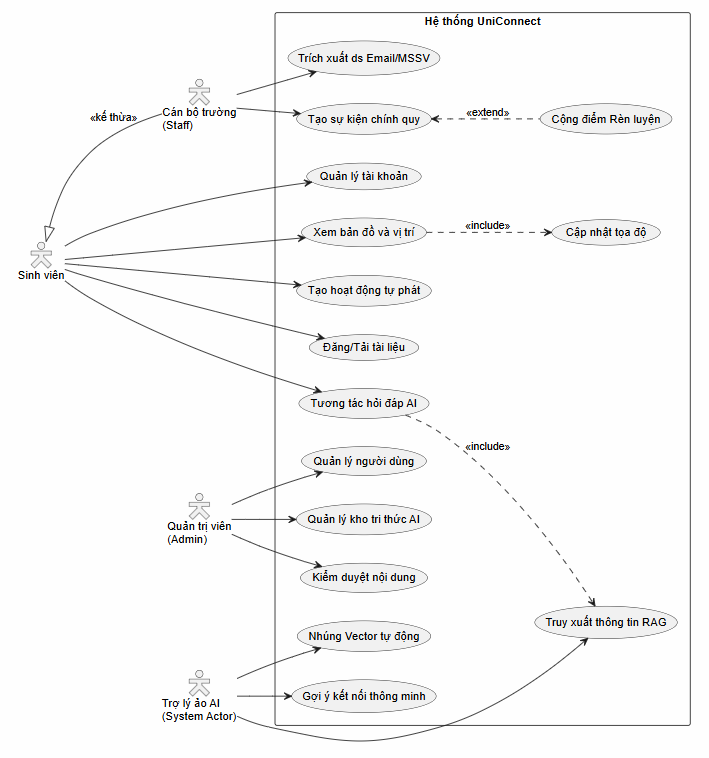
\includegraphics[width=0.85\textwidth]{Images/use-case-tong-quat.png}
    \caption{Sơ đồ Use Case tổng quát hệ thống UniConnect}
    \label{fig:usecase_tongquat}
\end{figure}

\subsection{Đặc tả Use case}
\subsubsection{Tạo hoạt động trên bản đồ}

\begin{figure}[H]
    \centering
    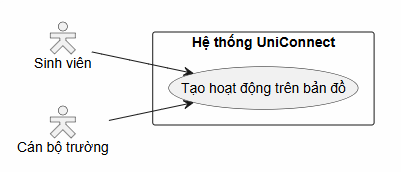
\includegraphics[width=0.85\textwidth]{Images/use-case-tao-hoat-dong.png}
    \caption{Sơ đồ Use Case tạo hoạt động}
    \label{fig:usecase_tao_hoat_dong}
\end{figure}

\renewcommand{\arraystretch}{1.5} % Tăng khoảng cách giữa các dòng cho dễ nhìn
\begin{xltabular}{\textwidth}{|>{\bfseries}p{3.5cm}|X|}
    % Cấu hình Tiêu đề và Nhãn bảng
    \caption{Đặc tả Use case Tạo hoạt động trên bản đồ} \label{tab:uc_taohoatdong} \\
    \hline
    \endfirsthead
    \caption[]{Đặc tả Use case Tạo hoạt động trên bản đồ} \\
    \hline
    \endhead
    \hline
    \endfoot
    \hline
    \endlastfoot

    % Nội dung bảng
    Use case name & Tạo hoạt động trên bản đồ \\ \hline
    Actor & Sinh viên, Cán bộ trường \\ \hline
    Description & Cho phép người dùng khởi tạo một điểm ghim (Marker) đại diện cho một sự kiện hoặc hoạt động (học nhóm, thể thao, sự kiện khoa) tại một tọa độ cụ thể trên khuôn viên trường. \\ \hline
    Preconditions & Người dùng đã đăng nhập thành công vào hệ thống và cấp quyền truy cập vị trí cho trình duyệt/ứng dụng. \\ \hline
    Postconditions & Hệ thống lưu thông tin hoạt động vào cơ sở dữ liệu, tự động nhúng vector mô tả hoạt động và hiển thị điểm ghim mới lên bản đồ cho tất cả người dùng khác. \\ \hline
    
    % Phân rã Normal Flow để hỗ trợ ngắt trang
    \textbf{Normal Flow} & 1. Actor nhấn giữ (long-press) vào một vị trí cụ thể trên giao diện bản đồ. \\
    & 2. Hệ thống hiển thị biểu mẫu yêu cầu nhập thông tin hoạt động. \\ 
    & 3. Actor nhập dữ liệu: Tiêu đề, Mô tả, Thời gian bắt đầu và Số lượng giới hạn. \\ 
    & 4. Actor nhấn nút "Tạo hoạt động". \\ 
    & 5. Hệ thống gửi dữ liệu tọa độ và nội dung form lên Backend xử lý. \\ 
    & 6. Hệ thống lưu bản ghi vào CSDL và chạy ngầm tác vụ nhúng Vector cho phần mô tả. \\ 
    & 7. Hệ thống thông báo tạo thành công và tải lại lớp bản đồ để hiển thị Marker mới. \\ \hline
    
    Alternative flow & Actor bỏ trống các trường thông tin bắt buộc (Tiêu đề, Thời gian); hệ thống sẽ chặn việc gửi dữ liệu ở phía Frontend, hiển thị viền đỏ ở các ô nhập liệu và yêu cầu điền đầy đủ. \\ \hline
    Exception & Sự cố đường truyền hoặc hết phiên đăng nhập: Tại bước 5, nếu thiết bị mất mạng hoặc token JWT đã hết hạn, máy chủ sẽ không thể xử lý. Hệ thống hiển thị thông báo "Kết nối thất bại, vui lòng thử lại", đồng thời giữ nguyên các thông tin Actor đã nhập trên biểu mẫu để tránh mất dữ liệu. \\ \hline

\end{xltabular}

\subsubsection{Quản lý hoạt động}

\begin{figure}[H]
    \centering
    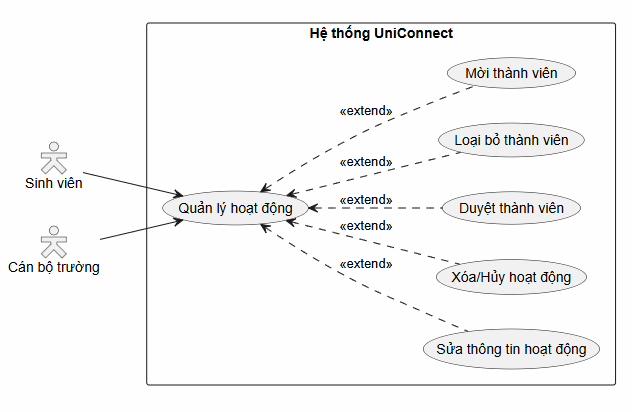
\includegraphics[width=0.85\textwidth]{Images/use-case-quan-ly-hoat-dong.png}
    \caption{Sơ đồ Use Case quản lý hoạt động}
    \label{fig:usecase_quan_ly_hoat_dong}
\end{figure}

\renewcommand{\arraystretch}{1.5} % Tăng khoảng cách dòng cho thoáng bảng
\begin{xltabular}{\textwidth}{|>{\bfseries}p{3.5cm}|X|}
    % Cấu hình Tiêu đề và Nhãn bảng (Tự động lặp lại tiêu đề nếu sang trang mới)
    \caption{Đặc tả Use case Quản lý hoạt động} \label{tab:uc_quanlyhoatdong} \\
    \hline
    \endfirsthead
    \caption[]{Đặc tả Use case Quản lý hoạt động} \\
    \hline
    \endhead
    \hline
    \endfoot
    \hline
    \endlastfoot

    % Kịch bản chi tiết bắt đầu từ đây
    Use case name & Quản lý hoạt động \\ \hline
    Actor & Sinh viên, Cán bộ trường (Chủ sở hữu hoạt động) \\ \hline
    Description & Cho phép người dùng quản lý các hoạt động hoặc sự kiện do chính mình khởi tạo trên bản đồ, bao gồm việc cập nhật thông tin, hủy hoạt động và điều phối danh sách thành viên tham gia. \\ \hline
    Preconditions & Actor đã đăng nhập thành công và hệ thống xác thực Actor chính là chủ sở hữu (người tạo) của hoạt động đó. \\ \hline
    Postconditions & Các thay đổi về thông tin hoạt động hoặc trạng thái thành viên được cập nhật đồng bộ vào cơ sở dữ liệu. \\ \hline
    
    % Bắt đầu phân rã hàng cho Normal Flow để tạo điểm ngắt trang
    \textbf{Normal Flow} & 1. Actor truy cập vào mục "Hoạt động của tôi" và chọn hoạt động cần điều phối. \\
    & 2. Hệ thống hiển thị bảng điều khiển quản lý (Dashboard) của hoạt động đó. \\ 
    & 3. Actor lựa chọn thực hiện một trong các nhánh hành động sau:
    \vspace{0.2cm}
    \begin{itemize}[leftmargin=*, noitemsep]
        \item \textbf{Nhánh Sửa thông tin:} Actor chọn "Chỉnh sửa", thay đổi các thông tin (Tiêu đề, Mô tả, Số lượng) và nhấn "Cập nhật". Hệ thống kiểm tra dữ liệu và lưu vào CSDL.
        \item \textbf{Nhánh Xóa/Hủy:} Actor chọn "Hủy hoạt động", hệ thống hiển thị hộp thoại cảnh báo. Actor nhấn "Xác nhận", hệ thống chuyển trạng thái sang "Đã hủy" và gỡ điểm ghim khỏi bản đồ.
        \item \textbf{Nhánh Duyệt thành viên:} Trong tab "Yêu cầu", Actor nhấn "Chấp nhận" đối với các sinh viên đang chờ. Hệ thống chuyển trạng thái của họ thành thành viên chính thức.
        \item \textbf{Nhánh Loại bỏ thành viên:} Trong tab "Thành viên", Actor chọn một sinh viên và nhấn "Loại bỏ khỏi nhóm". Hệ thống xóa sinh viên đó khỏi danh sách tham gia.
        \item \textbf{Nhánh Mời thành viên:} Actor nhập Mã số sinh viên/Email của người cần mời và nhấn "Gửi lời mời". Hệ thống gửi thông báo mời tham gia tới tài khoản mục tiêu.
    \end{itemize} \\ 
    & 4. Hệ thống hiển thị thông báo "Thao tác thành công" và cập nhật lại giao diện Dashboard. \\ \hline
    
    % Các mục cuối bảng
    Alternative flow & Tại bước 3, nếu Actor đang thực hiện dở dang một thao tác (ví dụ đang sửa thông tin hoặc đang mở hộp thoại xóa) nhưng nhấn nút "Quay lại" hoặc đóng tab, hệ thống sẽ hủy bỏ toàn bộ các thay đổi chưa lưu và quay về giao diện bước 2. \\ \hline
    Exception & Hoạt động đã bị khóa: Tại bước 1, nếu hoạt động này vừa bị Admin ẩn hoặc khóa do vi phạm nội dung ngay trước đó, hệ thống sẽ từ chối quyền truy cập, hiển thị thông báo "Hoạt động không còn khả dụng" và đưa Actor về trang chủ. \\ \hline

\end{xltabular}

\subsubsection{Tương tác với hoạt động}

\begin{figure}[H]
    \centering
    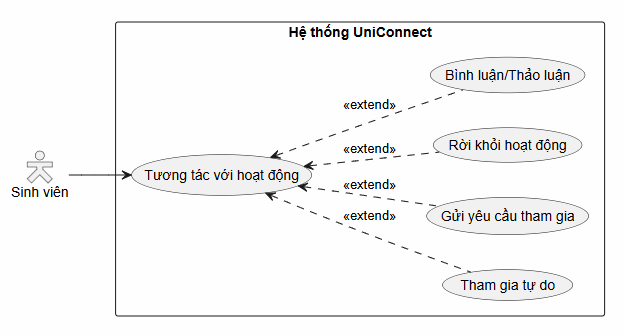
\includegraphics[width=0.85\textwidth]{Images/use-case-tuong-tac-hoat-dong.png} 
    \caption{Sơ đồ Use Case tham gia và tương tác hoạt động}
    \label{fig:usecase_tuong_tac_hoat_dong}
\end{figure}

\renewcommand{\arraystretch}{1.5}
\begin{xltabular}{\textwidth}{|>{\bfseries}p{3.5cm}|X|}
    % Cấu hình Tiêu đề và Nhãn bảng
    \caption{Đặc tả Use case Tham gia và tương tác hoạt động} \label{tab:uc_tuongtachoatdong} \\
    \hline
    \endfirsthead
    \caption[]{Đặc tả Use case Tham gia và tương tác hoạt động} \\
    \hline
    \endhead
    \hline
    \endfoot
    \hline
    \endlastfoot

    % Nội dung bảng
    Use case name & Tham gia và tương tác hoạt động \\ \hline
    Actor & Sinh viên \\ \hline
    Description & Cho phép Sinh viên tham gia vào các hoạt động trên bản đồ (có thể vào trực tiếp hoặc cần phê duyệt), rời khỏi hoạt động khi đổi ý, và thảo luận/bình luận bên trong không gian của hoạt động đó. \\ \hline
    Preconditions & Sinh viên đã đăng nhập hệ thống. Hoạt động mục tiêu đang trong trạng thái "Đang diễn ra" hoặc "Sắp diễn ra" (chưa kết thúc/chưa bị khóa). \\ \hline
    Postconditions & Trạng thái tham gia của Sinh viên được cập nhật (Đã tham gia/Đang chờ/Đã rời). Các bình luận (nếu có) được lưu vào cơ sở dữ liệu và hiển thị công khai cho những người xem hoạt động. \\ \hline
    
    % Phân rã Normal Flow để hỗ trợ ngắt trang
    \textbf{Normal Flow} & 1. Sinh viên nhấn vào một điểm ghim hoạt động trên giao diện bản đồ. \\ 
    & 2. Hệ thống hiển thị bảng thông tin chi tiết của hoạt động (Mô tả, Danh sách thành viên, Khu vực thảo luận). \\ 
    & 3. Tùy thuộc vào thiết lập của hoạt động và trạng thái hiện tại của Sinh viên, Sinh viên thực hiện một trong các nhánh sau:
    \vspace{0.2cm}
    \begin{itemize}[leftmargin=*, noitemsep]
        \item \textbf{Nhánh Tham gia tự do:} (Hoạt động không yêu cầu duyệt). Sinh viên nhấn "Tham gia". Hệ thống lập tức thêm Sinh viên vào danh sách thành viên chính thức.
        \item \textbf{Nhánh Xin tham gia:} (Hoạt động yêu cầu phê duyệt). Sinh viên nhấn "Xin tham gia". Hệ thống ghi nhận trạng thái "Đang chờ duyệt" và gửi thông báo (Notification) đến chủ sở hữu hoạt động.
        \item \textbf{Nhánh Rời khỏi:} Sinh viên (đang là thành viên hoặc đang chờ duyệt) nhấn nút "Rời khỏi". Hệ thống yêu cầu xác nhận, sau đó xóa Sinh viên khỏi danh sách tham gia.
        \item \textbf{Nhánh Bình luận:} Sinh viên nhập nội dung vào ô thảo luận và nhấn "Gửi". Hệ thống lưu bình luận vào CSDL và tự động cập nhật hiển thị lên luồng thảo luận.
    \end{itemize} \\ 
    & 4. Hệ thống hiển thị thông báo "Thao tác thành công" (hoặc "Đã gửi yêu cầu") và tải lại giao diện chi tiết hoạt động để cập nhật dữ liệu mới nhất. \\ \hline
    
    Alternative flow & Ở nhánh Bình luận, nếu Sinh viên chỉ nhập các khoảng trắng hoặc để trống ô nội dung, hệ thống (Frontend) sẽ vô hiệu hóa nút "Gửi" hoặc báo lỗi "Nội dung bình luận không được để trống" để ngăn chặn việc gửi dữ liệu rác. \\ \hline
    Exception & Đã đạt giới hạn số lượng thành viên: Tại nhánh Tham gia (hoặc Xin tham gia), sau khi Sinh viên nhấn nút, hệ thống (Backend) kiểm tra thấy số lượng người đăng ký đã đạt mức tối đa (max\_participants). Hệ thống chặn thao tác, không lưu dữ liệu và hiển thị thông báo lỗi: "Hoạt động này đã đủ số lượng người tham gia". \\ \hline

\end{xltabular}

\subsubsection{Đăng tải tài liệu}

\begin{figure}[H]
    \centering
    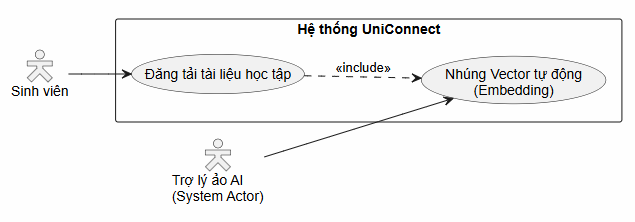
\includegraphics[width=0.85\textwidth]{Images/use-case-dang-tai-tai-lieu.png} 
    \caption{Sơ đồ Use Case Đăng tải tài liệu}
    \label{fig:usecase_dang_tai_tai_lieu}
\end{figure}

\renewcommand{\arraystretch}{1.5}
\begin{xltabular}{\textwidth}{|>{\bfseries}p{3.5cm}|X|}
    % Cấu hình Tiêu đề và Nhãn bảng
    \caption{Đặc tả Use case Đăng tải tài liệu và Nhúng tri thức} \label{tab:uc_dangtaitailieu} \\
    \hline
    \endfirsthead
    \caption[]{Đặc tả Use case Đăng tải tài liệu và Nhúng tri thức} \\
    \hline
    \endhead
    \hline
    \endfoot
    \hline
    \endlastfoot

    % Nội dung bảng
    Use case name & Đăng tải tài liệu và Nhúng tri thức (Embedding) \\ \hline
    Actor & Sinh viên, Trợ lý ảo AI (System Actor) \\ \hline
    Description & Cho phép Sinh viên đóng góp tài liệu học tập (PDF, Slide, Word) lên hệ thống. Đồng thời, hệ thống AI sẽ tự động đọc, phân tích và chuyển hóa nội dung tài liệu thành các Vector toán học để phục vụ công tác tra cứu ngữ nghĩa (Semantic Search) sau này. \\ \hline
    Preconditions & Sinh viên đã đăng nhập thành công. Tệp tin tải lên không chứa mã độc (được quét qua ở tầng Frontend/Firewall). \\ \hline
    Postconditions & Thông tin tài liệu được lưu trữ. File vật lý được lưu trữ an toàn (ví dụ: ổ cứng hoặc S3). Nội dung tài liệu được chuyển đổi thành Vector và lưu vào bảng cấu hình của cơ sở dữ liệu. \\ \hline
    
    % Phân rã Normal Flow để hỗ trợ ngắt trang
    \textbf{Normal Flow} & 1. Sinh viên truy cập vào phân hệ "Kho học liệu" và nhấn nút "Tải lên tài liệu". \\ 
    & 2. Hệ thống hiển thị biểu mẫu yêu cầu: Chọn tệp tin, Tiêu đề, Chọn Khoa/Ngành, và Gắn thẻ (Tags). \\ 
    & 3. Sinh viên đính kèm tệp và điền đầy đủ thông tin, sau đó nhấn "Đăng tải". \\ 
    & 4. Máy chủ (Backend) tiếp nhận yêu cầu, kiểm tra định dạng và kích thước tệp tin. \\ 
    & 5. Máy chủ lưu file vật lý vào hệ thống lưu trữ và tạo một bản ghi siêu dữ liệu (Metadata) vào cơ sở dữ liệu. \\ 
    & 6. Kích hoạt AI: Máy chủ đưa tác vụ đọc file vào hàng đợi. Trợ lý ảo AI (Worker) bóc tách văn bản từ file, chia nhỏ (Chunking) và gọi mô hình AI để chuyển văn bản thành Vector. \\ 
    & 7. Trợ lý AI lưu tọa độ Vector vào trường \texttt{embed} của hàng tài liệu tương ứng trong CSDL PostgreSQL. \\ 
    & 8. Hệ thống phản hồi "Đăng tải thành công" tới giao diện của Sinh viên. \\ \hline
    
    Alternative flow & Định dạng tệp không được hỗ trợ: Tại bước 3, nếu Sinh viên đính kèm các tệp thực thi (như .exe, .sh) hoặc các định dạng không phải văn bản/ảnh chuẩn, Frontend sẽ chặn lập tức và báo lỗi "Chỉ hỗ trợ tải lên định dạng PDF, DOCX, PPTX". \\ \hline
    Exception & Vượt quá dung lượng cho phép: Tại bước 4, nếu tệp tin có kích thước lớn hơn mức cấu hình hệ thống (ví dụ: lớn hơn 25MB), máy chủ sẽ từ chối xử lý luồng để bảo vệ băng thông và trả về thông báo lỗi "Dung lượng tệp vượt quá giới hạn". \\ \hline

\end{xltabular}

\subsubsection{Tương tác tài liệu}

\begin{figure}[H]
    \centering
    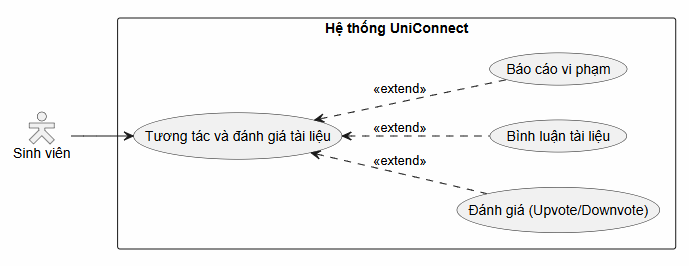
\includegraphics[width=0.85\textwidth]{Images/use-case-tuong-tac-tai-lieu.png} 
    \caption{Sơ đồ Use Case tương tác tài liệu}
    \label{fig:usecase_tuong_tac_tai_lieu}
\end{figure}

\renewcommand{\arraystretch}{1.5}
\begin{xltabular}{\textwidth}{|>{\bfseries}p{3.5cm}|X|}
    % Cấu hình Tiêu đề và Nhãn bảng
    \caption{Đặc tả Use case Tương tác tài liệu} \label{tab:uc_tuongtactailieu} \\
    \hline
    \endfirsthead
    \caption[]{Đặc tả Use case Tương tác tài liệu} \\
    \hline
    \endhead
    \hline
    \endfoot
    \hline
    \endlastfoot

    % Nội dung bảng
    Use case name & Tương tác và đánh giá tài liệu \\ \hline
    Actor & Sinh viên \\ \hline
    Description & Cho phép Sinh viên tương tác trực tiếp với các tài liệu trong kho học liệu thông qua các hành động bày tỏ quan điểm (Upvote/Downvote), để lại ý kiến thảo luận (Bình luận) hoặc gửi cảnh báo lên hệ thống khi phát hiện tài liệu có nội dung không phù hợp (Báo cáo vi phạm). \\ \hline
    Preconditions & Sinh viên đã đăng nhập thành công vào hệ thống và tài liệu mục tiêu đang ở trạng thái hiển thị công khai. \\ \hline
    Postconditions & Số lượt upvote/downvote được cập nhật, nội dung bình luận được hiển thị công khai, hoặc biểu mẫu báo cáo được chuyển tới phân hệ quản trị của Admin. \\ \hline
    
    % Phân rã Normal Flow để hỗ trợ ngắt trang
    \textbf{Normal Flow} & 1. Sinh viên chọn xem một tài liệu cụ thể trong giao diện Kho học liệu. \\ 
    & 2. Hệ thống hiển thị trang thông tin chi tiết của tài liệu, bao gồm nội dung xem trước, điểm đánh giá hiện tại, danh sách các bình luận cũ và tùy chọn báo cáo. \\ 
    & 3. Sinh viên thực hiện một trong các tương tác theo nhu cầu:
    \vspace{0.2cm}
    \begin{itemize}[leftmargin=*, noitemsep]
        \item \textbf{Nhánh Đánh giá (Upvote/Downvote):} Sinh viên nhấn vào biểu tượng tương ứng. Hệ thống ghi nhận, tính toán lại tổng điểm tài liệu và cập nhật trạng thái hiển thị của nút bấm ngay lập tức trên giao diện.
        \item \textbf{Nhánh Bình luận:} Sinh viên nhập ý kiến vào khung thảo luận và nhấn "Gửi". Hệ thống lưu dữ liệu và đưa bình luận mới vào đầu luồng hiển thị.
        \item \textbf{Nhánh Báo cáo vi phạm:} Sinh viên nhấn nút "Báo cáo", lựa chọn lý do vi phạm (tài liệu sai kiến thức, bản quyền, nội dung nhạy cảm) và nhập mô tả chi tiết, sau đó nhấn "Gửi báo cáo".
    \end{itemize} \\ 
    & 4. Hệ thống thực hiện lưu trữ các thay đổi tương ứng vào cơ sở dữ liệu và hiển thị thông báo "Thao tác thành công". \\ \hline
    
    Alternative flow & Hủy đánh giá: Ở nhánh Đánh giá, nếu Sinh viên nhấn lại vào nút bấm đang chọn (ví dụ đang Upvote và nhấn lại Upvote), hệ thống sẽ hiểu là hành động rút lại tương tác, trừ đi một điểm đánh giá và trả nút bấm về trạng thái mặc định. \\ \hline
    Exception & Tài liệu bị gỡ bỏ đột ngột: Tại bước 3, nếu tài liệu vừa bị tác giả chủ sở hữu hoặc Admin xóa/ẩn đi do vi phạm ngay tại thời điểm Sinh viên đang thao tác tương tác, Backend sẽ từ chối xử lý, trả về lỗi và Frontend hiển thị thông báo "Tài liệu này không còn tồn tại trên hệ thống". \\ \hline

\end{xltabular}

\begin{figure}[H]
    \centering
    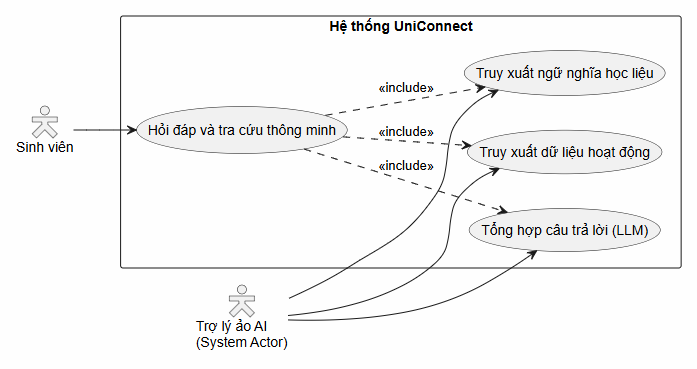
\includegraphics[width=0.85\textwidth]{Images/use-case-hoi-dap-chatbot.png} 
    \caption{Sơ đồ Use Case Hỏi đáp tri thức và tra cứu thông minh}
    \label{fig:usecase_tracuuthongminh}
\end{figure}

\renewcommand{\arraystretch}{1.5}
\begin{xltabular}{\textwidth}{|>{\bfseries}p{3.5cm}|X|}
    % Cấu hình Tiêu đề và Nhãn bảng
    \caption{Đặc tả Use case Hỏi đáp tri thức và tra cứu thông minh (RAG)} \label{tab:uc_tracuuthongminh} \\
    \hline
    \endfirsthead
    \caption[]{Đặc tả Use case Hỏi đáp tri thức và tra cứu thông minh} \\
    \hline
    \endhead
    \hline
    \endfoot
    \hline
    \endlastfoot

    % Nội dung bảng
    Use case name & Hỏi đáp tri thức và tra cứu thông minh \\ \hline
    Actor & Sinh viên, Trợ lý ảo AI (System Actor) \\ \hline
    Description & Cho phép Sinh viên đặt các câu hỏi tự nhiên về quy định nhà trường, tài liệu học thuật hoặc các hoạt động/sự kiện đang và sắp diễn ra trên bản đồ campus. Hệ thống ứng dụng kiến trúc RAG để tìm kiếm ngữ nghĩa đa nền tảng dữ liệu và phản hồi thông tin chính xác. \\ \hline
    Preconditions & Sinh viên đã đăng nhập thành công. Kho tri thức (quy chế, tài liệu) và siêu dữ liệu hoạt động (vị trí, mô tả sự kiện) đã được nhúng thành Vector và lưu trữ sẵn sàng. \\ \hline
    Postconditions & Sinh viên nhận được câu trả lời tổng hợp chính xác theo thời gian thực kèm các gợi ý liên kết (tới file tài liệu hoặc vị trí ghim sự kiện trên bản đồ). \\ \hline
    
    \textbf{Normal Flow} & 1. Sinh viên nhập câu hỏi vào khung chat (ví dụ: "Thủ tục mượn sách thư viện?" hoặc "Chiều nay ở sân thể chất có hoạt động nào không?") và nhấn gửi. \\ 
    & 2. Hệ thống tiếp nhận chuỗi văn bản và gọi mô hình Embedding để chuyển câu hỏi thành một Vector truy vấn. \\ 
    & 3. Giai đoạn phân loại và truy xuất dữ liệu hỗn hợp: Trợ lý AI thực hiện tìm kiếm khoảng cách Vector đồng thời trên các phân bảng lưu trữ của \texttt{pgvector} (bao gồm bảng phân đoạn tài liệu học liệu và bảng thông tin mô tả hoạt động). \\ 
    & 4. Trợ lý AI chọn lọc ra top các kết quả có độ tương đồng ngữ nghĩa cao nhất để làm ngữ cảnh nền tảng (Context). \\ 
    & 5. Giai đoạn tổng hợp ngữ cảnh: Hệ thống đóng gói câu hỏi gốc cùng với ngữ cảnh thu được thành một cấu trúc Prompt chuẩn mực và chuyển tiếp đến Mô hình ngôn ngữ lớn (LLM). \\ 
    & 6. LLM phân tích, tổng hợp dữ liệu và sinh ra câu trả lời bằng ngôn ngữ tự nhiên. \\ 
    & 7. Hệ thống hiển thị câu trả lời trực quan lên màn hình chat của Sinh viên (kèm đường dẫn đến điểm ghim hoạt động hoặc tệp tài liệu được nhắc tới) và lưu vào lịch sử hội thoại. \\ \hline
    
    Alternative flow & Nếu câu hỏi mang tính chất giao tiếp thông thường không chứa thực thể cần tra cứu, hệ thống bỏ qua bước truy xuất dữ liệu ở bước 3 và bước 4, chuyển trực tiếp câu hỏi sang cho LLM phản hồi theo luồng hội thoại thông thường. \\ \hline
    Exception & Tri thức nằm ngoài phạm vi hệ thống: Tại bước 3, nếu điểm số tương đồng ngữ nghĩa (Semantic Score) của tất cả các kết quả trả về từ cơ sở dữ liệu đều dưới ngưỡng an toàn cấu hình (ví dụ < 0.65), Trợ lý AI sẽ chủ động chặn luồng gửi đi của LLM nhằm chống ảo giác thông tin và đưa ra câu trả lời chuẩn: "Xin lỗi, hệ thống chưa tìm thấy thông tin phù hợp về quy định hoặc hoạt động này trong cơ sở dữ liệu." \\ \hline

\end{xltabular}

\subsubsection{Quản trị và kiểm duyệt}

\begin{figure}[H]
    \centering
    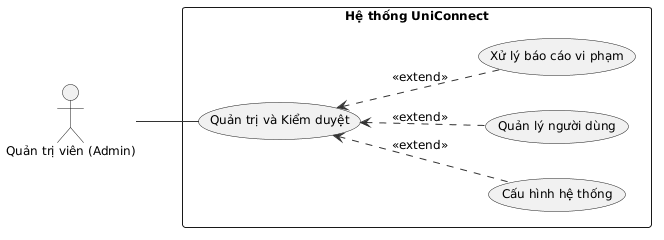
\includegraphics[width=0.85\textwidth]{Images/use-case-quan-tri.png} 
    \caption{Sơ đồ Use Case Quản trị hệ thống và Kiểm duyệt}
    \label{fig:usecase_quantri}
\end{figure}

\renewcommand{\arraystretch}{1.5}
\begin{xltabular}{\textwidth}{|>{\bfseries}p{3.5cm}|X|}
    % Cấu hình Tiêu đề và Nhãn bảng
    \caption{Đặc tả Use case Quản trị hệ thống và Kiểm duyệt} \label{tab:uc_quantri} \\
    \hline
    \endfirsthead
    \caption[]{Đặc tả Use case Quản trị hệ thống và Kiểm duyệt} \\
    \hline
    \endhead
    \hline
    \endfoot
    \hline
    \endlastfoot

    % Nội dung bảng
    Use case name & Quản trị hệ thống và Kiểm duyệt \\ \hline
    Actor & Quản trị viên (Admin) \\ \hline
    Description & Cung cấp bộ công cụ toàn diện để Admin giám sát nội dung cộng đồng, xử lý các báo cáo vi phạm từ người dùng, quản lý tài khoản và thiết lập các thông số vận hành của hệ thống. \\ \hline
    Preconditions & Admin đã xác thực thành công vào trang quản trị (Admin Dashboard) với tài khoản có quyền cao nhất. \\ \hline
    Postconditions & Các nội dung vi phạm bị gỡ bỏ, trạng thái tài khoản người dùng được cập nhật (khóa/mở), hoặc các thay đổi cấu hình được áp dụng vào cơ sở dữ liệu. \\ \hline
    
    % Phân rã Normal Flow để hỗ trợ ngắt trang
    \textbf{Normal Flow} & 1. Admin truy cập vào giao diện bảng điều khiển quản trị. \\ 
    & 2. Hệ thống hiển thị các số liệu thống kê tổng quan và danh sách các báo cáo vi phạm (Report List) đang chờ xử lý. \\ 
    & 3. Admin lựa chọn thực hiện một trong các nhánh nghiệp vụ sau:
    \vspace{0.2cm}
    \begin{itemize}[leftmargin=*, noitemsep]
        \item \textbf{Nhánh Xử lý vi phạm:} Admin xem chi tiết một báo cáo (chứa ID tài liệu hoặc hoạt động bị tố cáo). Nếu xác định vi phạm, Admin nhấn "Gỡ bỏ nội dung" và gửi cảnh cáo. Hệ thống sẽ ẩn dữ liệu này khỏi luồng hiển thị công khai.
        \item \textbf{Nhánh Quản lý người dùng:} Admin tìm kiếm một Sinh viên/Cán bộ cụ thể, thực hiện đổi vai trò (Role) hoặc nhấn "Khóa tài khoản" nếu người này vi phạm nghiêm trọng.
        \item \textbf{Nhánh Cấu hình hệ thống:} Admin điều chỉnh các danh mục dùng chung (như thêm/xóa Ngành học, Thẻ tag) hoặc cấu hình tham số hệ thống.
    \end{itemize} \\ 
    & 4. Máy chủ (Backend) ghi nhận lệnh thao tác, kiểm tra quyền JWT của Admin và thực thi thay đổi vào cơ sở dữ liệu PostgreSQL. \\ 
    & 5. Hệ thống hiển thị thông báo "Cập nhật thành công", đồng thời lưu một bản ghi nhật ký (Audit Log) về hành động vừa thực hiện để phục vụ tra soát. \\ \hline
    
    Alternative flow & Bác bỏ báo cáo: Ở nhánh Xử lý vi phạm, nếu Admin nhận thấy nội dung bị báo cáo không hề vi phạm quy định, Admin chọn "Bỏ qua báo cáo". Hệ thống sẽ đóng trạng thái của báo cáo đó mà không ảnh hưởng gì đến nội dung gốc. \\ \hline
    Exception & Xung đột dữ liệu khi kiểm duyệt: Tại bước 3, nếu nội dung vi phạm đang được xem xét đã bị tác giả tự tay xóa ngay trước đó, hệ thống sẽ báo lỗi "Nội dung này không còn tồn tại" và tự động chuyển trạng thái của báo cáo thành "Đã đóng". \\ \hline

\end{xltabular}

\subsection{Kiến trúc tổng thể hệ thống}

\begin{figure}[H]
    \centering
    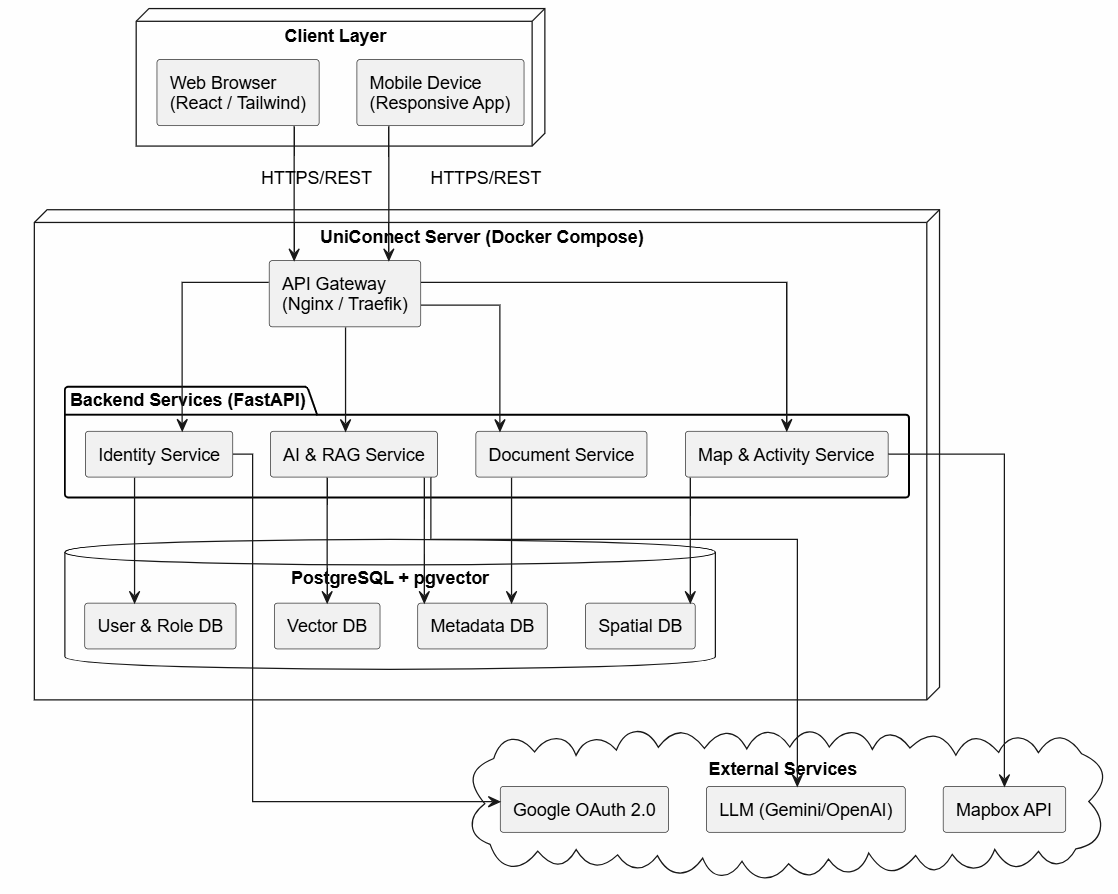
\includegraphics[width=0.85\textwidth]{Images/kien-truc-tong-the-he-thong.png} 
    \caption{Kiến trúc tổng thể hệ thống}
    \label{fig:kien_truc_tong_the_he_thong}
\end{figure}

Hệ thống UniConnect được thiết kế dựa trên kiến trúc hướng dịch vụ (Microservices), đảm bảo tính độc lập và khả năng mở rộng thông qua môi trường đóng gói container. Mọi yêu cầu từ phía Client đều đi qua API Gateway để điều hướng và kiểm soát truy cập. Về cơ chế xác thực, IdentityService tích hợp quy trình đăng nhập bảo mật, trong đó Client đảm nhiệm giao diện, còn Backend thực hiện cấp phát và xác thực JWT nội bộ qua kênh Server-to-Server, đảm bảo an toàn cho phiên làm việc. Đối với tính năng tra cứu thông minh, AI \& RAG Service đóng vai trò xử lý ngôn ngữ tự nhiên, đóng gói ngữ cảnh từ cơ sở dữ liệu Vector (pgvector) và quản lý lịch sử hội thoại trước khi gửi sang Mô hình ngôn ngữ lớn (LLM) để sinh câu trả lời. Các dịch vụ nghiệp vụ cốt lõi khác như Map \& Activity Service và Document Service hoạt động song song với phân vùng dữ liệu riêng biệt, đảm bảo sự tách biệt rõ ràng về mặt lưu trữ và logic xử lý giữa mạng xã hội bản đồ và kho học liệu.

\subsection{Mô tả mô hình thực thể kết hợp (ERD)}

\begin{figure}[H]
    \centering
    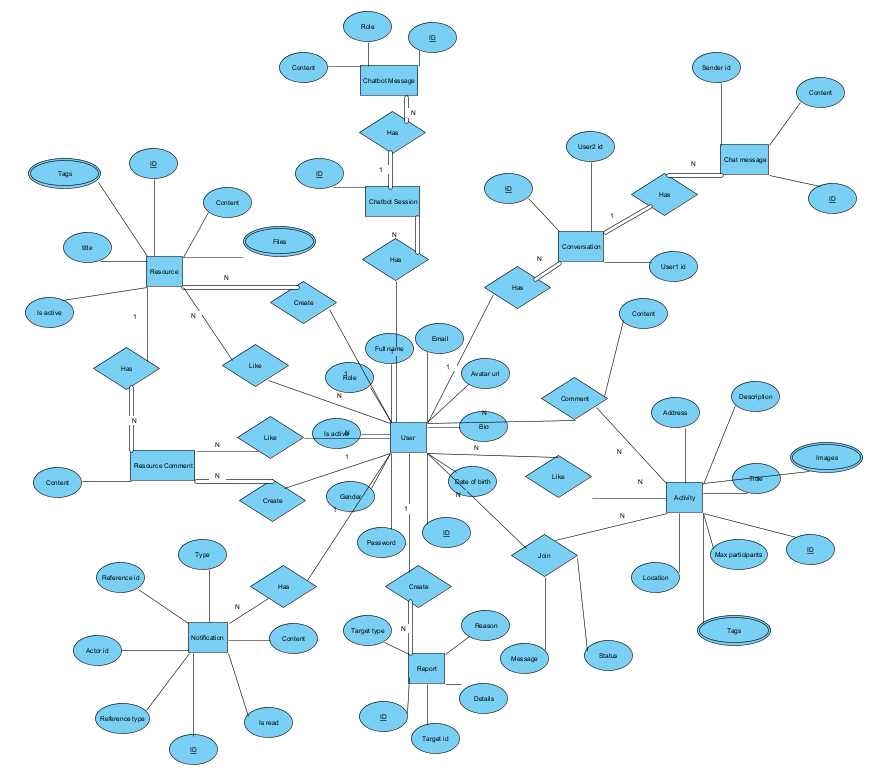
\includegraphics[width=0.85\textwidth]{Images/erd.png} 
    \caption{Entity Relationship Diagram của hệ thống}
    \label{fig:mo_hinh_erd}
\end{figure}

\subsubsection{Danh sách thực thể và thuộc tính}
\begin{enumerate}
    \item User
    Đại diện cho tất cả các tác nhân tham gia vào hệ thống UniConnect (bao gồm Sinh viên, Cán bộ trường và Quản trị viên). Thực thể này lưu trữ các thông tin cốt lõi để định danh, phân quyền và hồ sơ cá nhân của người dùng.
    \begin{itemize}
        \item ID: Mã định danh duy nhất (khóa chính), tự động tăng để quản lý người dùng.

        \item Email, Password: Thông tin tài khoản dùng để đăng nhập và mật khẩu đã được mã hóa để đảm bảo an toàn thông tin.
        
        \item Role: Vai trò của người dùng (Sinh viên, Cán bộ, hoặc Admin), quyết định quyền hạn truy cập các tính năng.
        
        \item Is Active: Trạng thái tài khoản (Cho phép hoặc Chặn truy cập).
        
        \item Full Name: Họ và tên đầy đủ của người dùng.
        
        \item Avatar URL: Đường dẫn liên kết tới hình ảnh đại diện (Lưu trữ trên Cloud hoặc Server).
        
        \item Gender, Date of Birth: Thông tin giới thiệu cơ bản về giới tính và ngày sinh.
        
        \item Bio: Đoạn giới thiệu ngắn về bản thân của người dùng.
        
        \item Created At, Updated At: (Từ TimestampMixin) Ghi lại thời điểm tạo tài khoản và lần cập nhật thông tin gần nhất.
    \end{itemize}

    \item Activity
    Thực thể này đại diện cho các sự kiện hoặc hoạt động được ghim trên bản đồ campus. Nó chứa toàn bộ thông tin về nội dung, thời gian và tọa độ địa lý để người dùng có thể tìm kiếm và tham gia.

    \begin{itemize}
        \item ID: Mã định danh duy nhất cho mỗi hoạt động.

        \item Owner ID: Khóa ngoại tham chiếu đến người tạo hoạt động (User).
        
        \item Title, Description: Tiêu đề và nội dung mô tả chi tiết về hoạt động.
        
        \item Images, Tags: Danh sách các đường dẫn ảnh minh họa và bộ thẻ từ khóa để phân loại hoạt động (ví dụ: \#thethao, \#hocthuat).
        
        \item Max Participants: Giới hạn số lượng người tham gia tối đa (nếu để trống nghĩa là không giới hạn).
        
        \item Address, Location: Địa chỉ văn bản và tọa độ địa lý thực tế (Point - vĩ độ/kinh độ). Đây là dữ liệu cốt lõi để hiển thị điểm ghim trên bản đồ.
        
        \item Start Time, End Time: Khung thời gian diễn ra hoạt động.
        
        \item Registration Deadline: Hạn chót để người dùng nhấn đăng ký tham gia.
        
        \item Auto Approve: Chế độ phê duyệt tự động. Nếu là True, người dùng nhấn tham gia sẽ vào thẳng danh sách; nếu False, chủ sở hữu phải duyệt thủ công.
        
        \item Is Active: Trạng thái hiển thị của hoạt động trên bản đồ.

        \item Created At, Updated At: (Từ TimestampMixin) Ghi lại thời điểm tạo hoạt động và lần cập nhật thông tin gần nhất.
    \end{itemize}

    \item Resource
    Thực thể này quản lý các bài viết, tài liệu học tập và tri thức được đóng góp bởi cộng đồng sinh viên hoặc cán bộ trường. Đây là nguồn dữ liệu chính để Trợ lý AI thực hiện truy xuất ngữ nghĩa.
    \begin{itemize}
        \item ID: Mã định danh duy nhất của tài liệu.

        \item Author ID: Khóa ngoại liên kết tới người đăng tải (User).
        
        \item Title: Tiêu đề của tài liệu/bài viết, giúp người dùng nhận diện nhanh nội dung.
        
        \item Content: Nội dung chi tiết của học liệu. Trường này hỗ trợ định dạng Markdown, cho phép trình bày văn bản phong phú, đính kèm hình ảnh và các liên kết tải xuống tài liệu vật lý (PDF, Slide, v.v.).
        
        \item Tags: Danh sách các từ khóa liên quan giúp phân loại và tìm kiếm tài liệu theo chủ đề hoặc môn học.
        
        \item Is Active: Trạng thái kiểm duyệt hoặc hiển thị của tài liệu trên hệ thống.

        \item Created At, Updated At: (Từ TimestampMixin) Ghi lại thời điểm tạo bài viết và lần cập nhật thông tin gần nhất.
    \end{itemize}

    \item Report
    Thực thể này quản lý các báo cáo từ người dùng đối với các nội dung khác trên hệ thống. Điểm đặc biệt của thực thể này là sử dụng cơ chế định danh mục tiêu linh hoạt, cho phép báo cáo nhiều loại đối tượng khác nhau (như hoạt động, tài liệu, hoặc bình luận).

    \begin{itemize}
        \item ID: Mã định danh duy nhất cho từng bản ghi báo cáo.

        \item Reporter ID: Khóa ngoại liên kết tới người thực hiện báo cáo (User).
        
        \item Target Type: Loại đối tượng bị báo cáo (Ví dụ: Resource, Activity, Comment). Đây là trường định danh để hệ thống biết báo cáo này thuộc phân hệ nào.
        
        \item Target ID: ID vật lý của đối tượng bị báo cáo trong bảng tương ứng của nó.
        
        \item Reason: Lý do báo cáo được chọn từ danh sách có sẵn (Ví dụ: Nội dung nhạy cảm, Thông tin sai lệch, Lừa đảo, Vi phạm bản quyền).
        
        \item Details: Nội dung mô tả chi tiết bổ sung từ người báo cáo để giúp Admin có thêm căn cứ xử lý.
        
        \item Status: Trạng thái xử lý của báo cáo (Đang chờ, Đã xử lý, hoặc Đã bác bỏ).
        
        \item Created At, Updated At: (Từ TimestampMixin) Ghi lại thời điểm tạo báo cáo và lần cập nhật thông tin gần nhất.
    \end{itemize}

    \item Notification
    Thực thể này quản lý luồng thông tin cập nhật giữa các người dùng và giữa hệ thống với người dùng. Nó đảm bảo tính tương tác thời gian thực bằng cách gửi thông điệp khi có sự thay đổi về trạng thái hoạt động hoặc các tương tác xã hội.
    \begin{itemize}
        \item ID: Mã định danh duy nhất cho mỗi thông báo.

        \item Recipient ID: (Khóa ngoại) Định danh người nhận thông báo. Đây là quan hệ bắt buộc (Total Participation).
        
        \item Actor ID: (Khóa ngoại) Định danh người gây ra hành động dẫn đến thông báo (ví dụ: người nhấn "Like" hoặc "Comment"). Trường này có thể để trống (NULL) nếu là thông báo từ hệ thống.
        
        \item Type: Phân loại thông báo dựa trên tập giá trị NotificationType (Yêu cầu tham gia, Được duyệt, Cập nhật hoạt động, Bình luận mới, Cảm xúc mới, Thông báo hệ thống).
        
        \item Reference ID \& Type: Cặp thuộc tính dùng để dẫn hướng người dùng khi nhấn vào thông báo. Reference Type xác định đối tượng liên quan (Activity, Resource, hoặc User), và Reference ID lưu ID của đối tượng đó.
        
        \item Content: Nội dung chi tiết của thông báo hiển thị cho người dùng.
        
        \item Is Read: Trạng thái kiểm soát việc người dùng đã xem thông báo hay chưa, phục vụ cho việc hiển thị dấu chấm đỏ hoặc số lượng thông báo mới trên giao diện UI.
    \end{itemize}

    \item Conversation
    Thực thể này đóng vai trò là "phòng chat" đại diện cho kênh kết nối trực tiếp giữa hai người dùng. Thay vì tạo nhiều bản ghi trùng lặp, thực thể này quản lý một cặp định danh duy nhất để duy trì lịch sử hội thoại xuyên suốt.
    \begin{itemize}
        \item ID: Mã định danh duy nhất của cuộc hội thoại.
        
        \item User1 ID \& User2 ID: Hai khóa ngoại tham chiếu đến bảng User. Hệ thống áp dụng ràng buộc UniqueConstraint và CheckConstraint ($user1\_id < user2\_id$) để đảm bảo giữa hai người dùng bất kỳ chỉ tồn tại duy nhất một phòng chat, tránh lãng phí dữ liệu.
        
        \item Last Message At: Thuộc tính lưu thời điểm tin nhắn cuối cùng được gửi. Đây là dữ liệu quan trọng để hệ thống sắp xếp (sort) danh sách hộp thư, đưa các cuộc hội thoại mới nhất lên đầu giao diện.
    \end{itemize}

    \item Chatbot session
    Thực thể này đóng vai trò là một "ngữ cảnh hội thoại" giữa người dùng và Trợ lý AI. Việc chia theo từng phiên giúp người dùng quản lý các chủ đề hỏi đáp khác nhau (ví dụ: một phiên hỏi về học phí, một phiên hỏi về sơ đồ trường) mà không bị lẫn lộn nội dung.
    \begin{itemize}
        \item ID: Mã định danh duy nhất của phiên chat.

        \item User ID: Khóa ngoại liên kết tới người sở hữu phiên chat. Một người dùng có thể có nhiều phiên hỏi đáp khác nhau.
        
        \item Title: Tiêu đề của phiên chat, thường được hệ thống tự động sinh ra từ câu hỏi đầu tiên để người dùng dễ dàng tìm lại lịch sử.
        
        \item Created At: Thời điểm bắt đầu phiên hội thoại.
    \end{itemize}

    \item Chatbot message
    Lưu trữ chi tiết từng lượt trao đổi trong một phiên chat. Đây là nguồn dữ liệu quan trọng để hệ thống "nhắc lại" ngữ cảnh cho mô hình ngôn ngữ (LLM) trong các câu hỏi tiếp theo.
    \begin{itemize}
        \item ID: Mã định danh duy nhất của tin nhắn.

        \item Session ID: Khóa ngoại liên kết chặt chẽ với phiên chat tương ứng. Khi xóa phiên chat, toàn bộ tin nhắn liên quan sẽ bị xóa theo (Cascade).

        \item Role: Vai trò của thực thể gửi tin nhắn (User - Người dùng hoặc Assistant - Trợ lý AI). Đây là thông tin bắt buộc để AI hiểu đâu là câu hỏi và đâu là câu trả lời cũ.

        \item Content: Nội dung văn bản của tin nhắn.

        \item Created At: Ghi lại thời gian để sắp xếp thứ tự các câu thoại theo đúng trình tự thời gian.
    \end{itemize}
\end{enumerate}

\subsubsection{Mô tả các mối quan hệ}

\setlist[itemize]{leftmargin=*, nosep, topsep=0pt} % Tối ưu khoảng cách trong list

\begin{longtable}{|p{0.25\textwidth}|p{0.15\textwidth}|p{0.53\textwidth}|}
    \caption{Bảng tổng hợp các mối quan hệ giữa các thực thể trong hệ thống} \label{tab:relationship_summary} \\
    
    \hline
    \textbf{Thực thể tham gia} & \textbf{Quan hệ} & \textbf{Giải thích ý nghĩa \& Ràng buộc} \\ \hline
    \endfirsthead

    \hline
    \endlastfoot

    % --- Dữ liệu bảng ---
    \textbf{User -- Activity} & \textbf{Create} \newline (1 -- N) & 
    \begin{itemize}
        \item Một \textbf{User} có thể tổ chức/quản lý nhiều \textbf{Activity}.
        \item Một \textbf{Activity} bắt buộc phải được sở hữu bởi duy nhất một \textbf{User} (Owner).
    \end{itemize} \\ \hline
    
    \textbf{User -- Activity} & \textbf{Participate} \newline (N -- N) & 
    \begin{itemize}
        \item Một \textbf{User} có thể tham gia nhiều \textbf{Activity} khác nhau.
        \item Một \textbf{Activity} có thể có nhiều người tham gia thông qua thực thể trung gian \textbf{ActivityParticipant}.
    \end{itemize} \\ \hline

    \textbf{User -- Resource} & \textbf{Create} \newline (1 -- N) & 
    \begin{itemize}
        \item Một \textbf{User} có thể đăng tải nhiều tài liệu học tập (\textbf{Resource}).
        \item Một \textbf{Resource} bắt buộc phải thuộc về một tác giả xác định.
    \end{itemize} \\ \hline

    \textbf{User -- Resource} & \textbf{Like} \newline (1 -- N) & 
    \begin{itemize}
        \item Một \textbf{User} có thể thích nhiều tài liệu học tập (\textbf{Resource}).
        \item Một \textbf{Resource} có thể được thích bởi nhiều người dùng.
    \end{itemize} \\ \hline

    \textbf{User -- Resource} & \textbf{Comment} \newline (1 -- N) & 
    \begin{itemize}
        \item Một \textbf{User} có thể bình luận trong nhiều tài liệu học tập (\textbf{Resource}).
        \item Một \textbf{Resource} có thể nhận bình luận bởi nhiều người dùng.
    \end{itemize} \\ \hline

    \textbf{Conversation -- Message} & \textbf{Has} \newline (1 -- N) & 
    \begin{itemize}
        \item Một cuộc hội thoại (\textbf{Has}) chứa nhiều tin nhắn \textbf{DirectMessage}.
        \item Một \textbf{DirectMessage} bắt buộc phải nằm trong một cuộc hội thoại cụ thể.
    \end{itemize} \\ \hline

    \textbf{User -- Chatbot Session} & \textbf{Has} \newline (1 -- N) & 
    \begin{itemize}
        \item Một \textbf{User} có thể khởi tạo nhiều phiên hỏi đáp với Trợ lý AI (\textbf{ChatSession}).
        \item Mỗi phiên chat bắt buộc gắn liền với một người dùng cụ thể.
    \end{itemize} \\ \hline

    \textbf{User -- Conversation} & \textbf{Has} \newline (1 -- N) & 
    \begin{itemize}
        \item Một \textbf{User} có thể khởi tạo nhiều phiên trò chuyện với những người dùng khác.
        \item Mỗi phiên chat bắt buộc gắn liền với một người dùng cụ thể.
    \end{itemize} \\ \hline

    \textbf{ChatSession -- Message} & \textbf{Has} \newline (1 -- N) & 
    \begin{itemize}
        \item Một phiên hỏi đáp (\textbf{ChatSession}) bao gồm nhiều lượt gửi tin nhắn \textbf{ChatMessage}.
        \item Mỗi \textbf{ChatMessage} lưu trữ nội dung hội thoại theo vai trò (User/Assistant).
    \end{itemize} \\ \hline

    \textbf{User -- Notification} & \textbf{Has} \newline (1 -- N) & 
    \begin{itemize}
        \item Một \textbf{User} có thể nhận được nhiều thông báo (\textbf{Notification}).
        \item Mỗi thông báo được gửi đích danh đến một người nhận (Recipient).
    \end{itemize} \\ \hline

    \textbf{User -- Report} & \textbf{Create} \newline (1 -- N) & 
    \begin{itemize}
        \item Một \textbf{User} có thể gửi nhiều báo cáo vi phạm (\textbf{Report}).
        \item Một báo cáo bắt buộc phải được tạo bởi một \textbf{User} xác định.
    \end{itemize} \\ \hline

    \textbf{User -- Activity comment} & \textbf{Create} \newline (1 -- N) & 
    \begin{itemize}
        \item Một \textbf{User} có thể bình luận trên các nội dung.
        \item Một bình luận được tạo bởi một người dùng cụ thể.
    \end{itemize} \\ \hline
    
    \textbf{User -- Activity comment} & \textbf{Like} \newline (N -- N) & 
    \begin{itemize}
        \item Một \textbf{User} có thể thích bình luận trong nội dung.
        \item Một bình luận hoạt động được thích bởi nhiều người dùng.
    \end{itemize} \\ \hline
\end{longtable}

\subsection{Activity diagram}

\begin{figure}[H]
    \centering
    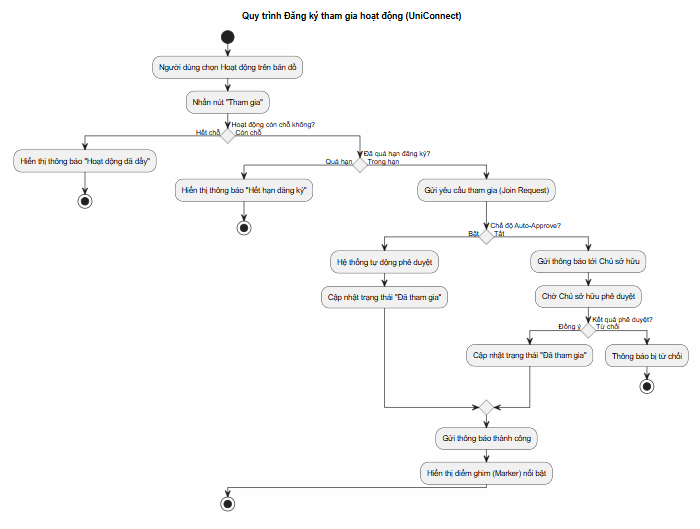
\includegraphics[width=0.85\textwidth]{Images/activity-join-activity.png} 
    \caption{Activity Diagram quy trình đăng ký tham gia hoạt động}
    \label{fig:activity_tham_gia_hoat_dong}
\end{figure}

\begin{figure}[H]
    \centering
    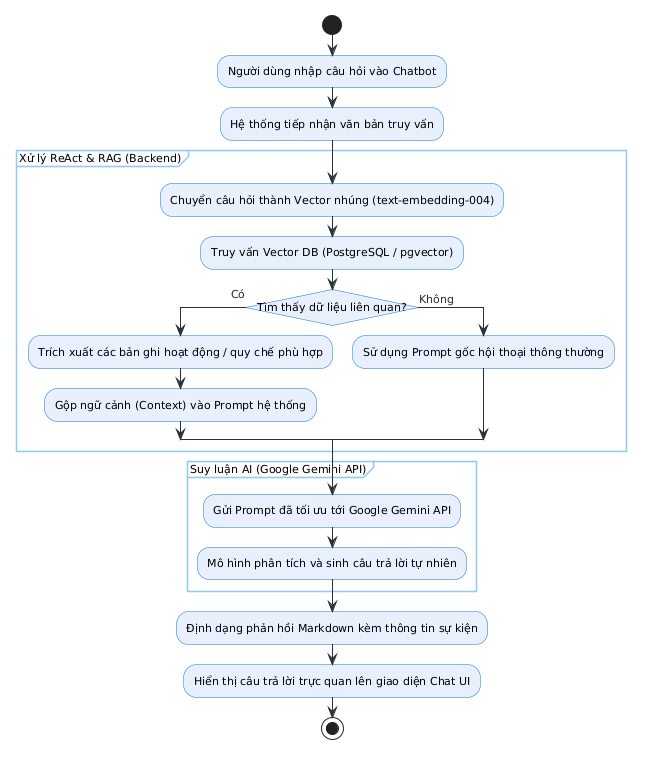
\includegraphics[width=0.85\textwidth]{Images/activity-hoi-chatbot.png} 
    \caption{Activity Diagram quy trình hỏi đáp với trợ lý AI}
    \label{fig:activity_hoi_dap_chatbot}
\end{figure}

\subsection{Sequence diagram}

\begin{figure}[H]
    \centering
    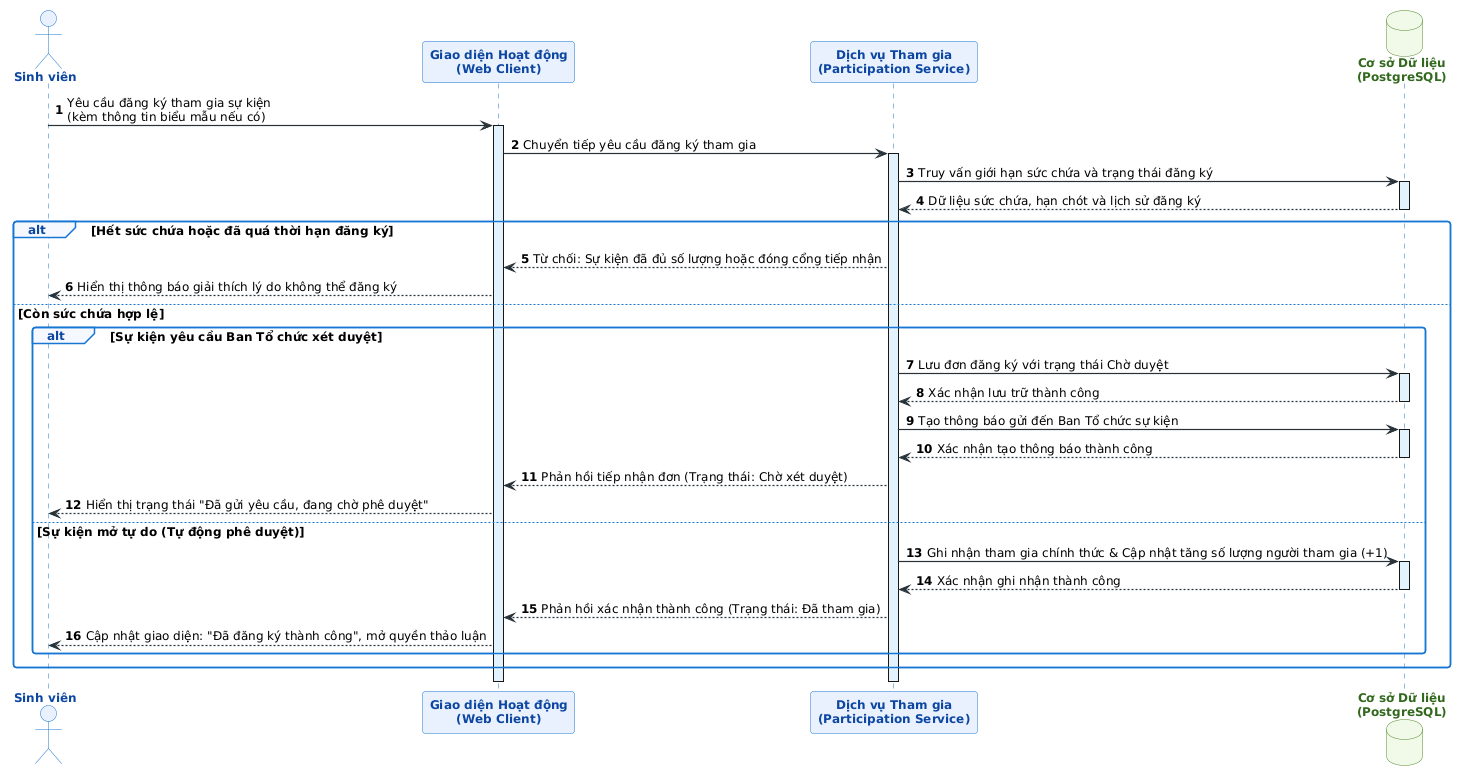
\includegraphics[width=0.85\textwidth]{Images/sequence_join_activity.png} 
    \caption{Sequence Diagram quy trình đăng ký tham gia hoạt động}
    \label{fig:sequence_tham_gia_hoat_dong}
\end{figure}

\begin{figure}[H]
    \centering
    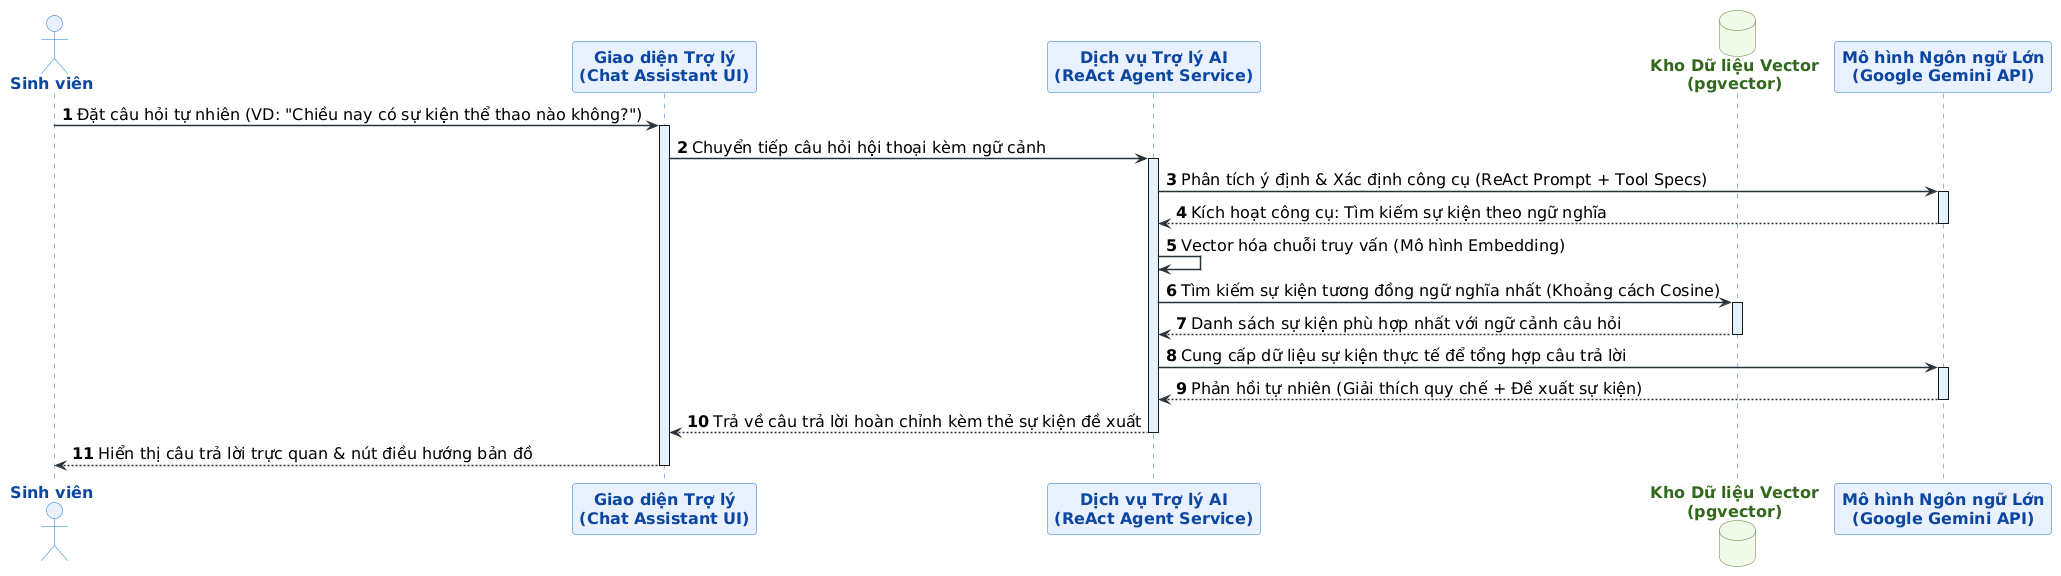
\includegraphics[width=0.85\textwidth]{Images/sequence-hoi-dap-chatbot.png} 
    \caption{Sequence Diagram quy trình hỏi đáp với trợ lý AI}
    \label{fig:sequence_hoi_dap_chatbot}
\end{figure}

\section{Hiện thực backend}

\subsection{Môi trường phát triển và công nghệ sử dụng}
\begin{itemize}
    \item Ngôn ngữ: Python 3.10+.

    \item Framework: FastAPI (đảm bảo hiệu năng cao, hỗ trợ Asynchronous).
    
    \item Database: PostgreSQL 15+ kết hợp với PostGIS (xử lý tọa độ bản đồ) và pgvector (xử lý Vector AI).
    
    \item ORM: SQLAlchemy 2.0 (quản lý truy vấn thông qua Model).
    
    \item Migration: Alembic (quản lý lịch sử thay đổi cấu trúc Database).
    
    \item Môi trường: Docker \& Docker-compose (để đóng gói và triển khai nhanh).
\end{itemize}

\subsection{Cấu trúc thư mục dự án}

Để đảm bảo tính linh hoạt, dễ bảo trì và khả năng mở rộng, mã nguồn của hệ thống Backend được tổ chức theo kiến trúc phân lớp (Layered Architecture). Cấu trúc thư mục chi tiết của dự án được trình bày như sau:

\begin{mycode}[Project Directory Structure]{}
uniconnect/
    app/
        api/                # API Layer (Routes)
            v1/             # API Version 1
                api.py      # Main router entry point
                endpoints/  # Specific endpoint logic (auth, activity, etc.)
        core/               # Core configurations (config, security)
        crud/               # Basic CRUD operations
        models/             # SQLAlchemy model definitions (ERD mapping)
        schemas/            # Pydantic schemas (Data Validation)
        services/           # Business logic layer (RAG, AI processing)
        db/                 # Database session management
        main.py             # Application entry point
    alembic/                # Database migrations management
    tests/                  # Automated test cases
    .env                    # Environment variables
    docker-compose.yml      # Container orchestration config
    Dockerfile              # Container image definition
    requirements.txt        # Python project dependencies
\end{mycode}

\subsection{Mô tả các thành phần hệ thống}
Việc tổ chức mã nguồn theo cấu trúc trên giúp tách biệt rõ ràng giữa logic nghiệp vụ, giao diện lập trình và truy xuất dữ liệu. Các thành phần chính bao gồm:

\begin{itemize}
    \item \textbf{Thư mục \texttt{app/models/}:} Hiện thực hóa sơ đồ ERD thành các lớp Python thông qua SQLAlchemy ORM. Tại đây, các ràng buộc dữ liệu, khóa chính, khóa ngoại và các kiểu dữ liệu đặc thù như \textit{Geography} (cho bản đồ) và \textit{Vector} (cho AI) được định nghĩa chặt chẽ.
    
    \item \textbf{Thư mục \texttt{app/api/}:} Đóng vai trò lớp biên (Boundary), định nghĩa các Endpoint để Frontend tương tác. Cách tiếp cận này giúp hệ thống có khả năng nâng cấp các phiên bản API độc lập mà không gây ảnh hưởng đến các thành phần cũ.
    
    \item \textbf{Thư mục \texttt{app/services/}:} Đây là lớp chứa đựng logic nghiệp vụ chính. Các xử lý phức tạp như: quy trình tìm kiếm ngữ nghĩa RAG, tính toán không gian bản đồ, hay logic phê duyệt người dùng tham gia hoạt động được tập trung tại đây để tối ưu hóa việc tái sử dụng mã nguồn.
    
    \item \textbf{Thư mục \texttt{app/schemas/}:} Sử dụng thư viện Pydantic để định nghĩa các cấu trúc dữ liệu trao đổi (DTO). Lớp này đảm bảo mọi dữ liệu đầu vào và đầu ra đều được kiểm tra kiểu dữ liệu (Validation) nghiêm ngặt trước khi xử lý.
    
    \item \textbf{Hệ thống \texttt{alembic/}:} Đảm nhận vai trò quản lý các phiên bản cấu trúc cơ sở dữ liệu. Mọi thay đổi trong mô hình dữ liệu đều được ghi vết và cập nhật đồng bộ vào Database thực tế thông qua các kịch bản Migration, đảm bảo tính toàn vẹn dữ liệu.
    
    \item \textbf{Docker và Containerization:} Toàn bộ hệ thống Backend và các dịch vụ bổ trợ (PostgreSQL, pgvector) được đóng gói trong các Container riêng biệt, giúp đồng nhất môi trường phát triển và môi trường vận hành thực tế.
\end{itemize}

\subsection{Hiện thực các tính năng cốt lõi}

\subsubsection{Xử lý dữ liệu không gian và Bản đồ (Geospatial Handling)}
Để quản lý các hoạt động trên bản đồ campus, hệ thống sử dụng tiện ích mở rộng \textit{PostGIS} của PostgreSQL kết hợp với thư viện \textit{GeoAlchemy2}. Dữ liệu tọa độ được lưu trữ dưới định dạng hình học \texttt{POINT} với hệ tọa độ \texttt{SRID 4326}.

\begin{mycode}[Geospatial Field Definition in Activity Model]{Python}
# Define geospatial Point field (latitude, longitude)
location = Column(Geography(geometry_type='POINT', srid=4326), nullable=True)

@property
def latitude(self):
    """Extract latitude from Geometry data"""
    if self.location is not None:
        return to_shape(self.location).y
    return None

@property
def longitude(self):
    """Extract longitude from Geometry data"""
    if self.location is not None:
        return to_shape(self.location).x
    return None
\end{mycode}

Việc hiện thực này cho phép hệ thống thực hiện các truy vấn không gian phức tạp như tìm kiếm các hoạt động trong bán kính nhất định xung quanh người dùng với hiệu năng tối ưu.

\subsubsection{Hệ thống tìm kiếm ngữ nghĩa và Trợ lý AI (RAG)}
Đây là tính năng trọng tâm của dự án, cho phép người dùng hỏi đáp dựa trên kho học liệu nội bộ. Hệ thống thực hiện quy trình RAG qua các bước:
\begin{enumerate}[leftmargin=*]
    \item \textbf{Vector hóa:} Sử dụng mô hình Embedding (như Sentence-Transformers hoặc Gemini) để chuyển đổi nội dung tài liệu thành các Vector 768 chiều.
    \item \textbf{Lưu trữ:} Sử dụng tiện ích \textit{pgvector} để lưu trữ và lập chỉ mục (Index) các Vector này.
    \item \textbf{Truy xuất:} Sử dụng toán tử khoảng cách Cosine (\textit{Cosine Similarity}) để tìm kiếm các đoạn văn bản có ý nghĩa gần nhất với câu hỏi của người dùng.
\end{enumerate}

\begin{mycode}[Vector Similarity Search Query]{SQL}
-- Find the top 5 chunks with similarity > 0.7
-- The <=> operator calculates Cosine Distance
-- Subtract from 1 to obtain Cosine Similarity
SELECT 
    content, 
    1 - (embedding <=> '[vector_query]') AS similarity
FROM resources
WHERE 1 - (embedding <=> '[vector_query]') > 0.7
ORDER BY similarity DESC 
LIMIT 5;
\end{mycode}

\subsubsection{Authentication}

Hệ thống triển khai cơ chế xác thực dựa trên tiêu chuẩn JSON Web Token (JWT). Mật khẩu người dùng được mã hóa bằng thuật toán bcrypt nhằm đảm bảo an toàn dữ liệu. Khi đăng nhập thành công, hệ thống cấp một mã định danh (Access Token) để người dùng thực hiện các yêu cầu tiếp theo thông qua lớp trung gian (Middleware).

\begin{mycode}[JWT and Password Security]{Python}
from jose import jwt
from passlib.context import CryptContext
from datetime import datetime, timedelta
Security configuration
pwd_context = CryptContext(schemes=["bcrypt"], deprecated="auto")
SECRET_KEY = "your_secret_key"
ALGORITHM = "HS256"

def create_access_token(data: dict):
"""Generate JWT for authenticated users"""
to_encode = data.copy()
expire = datetime.utcnow() + timedelta(minutes=30)
to_encode.update({"exp": expire})
return jwt.encode(to_encode, SECRET_KEY, algorithm=ALGORITHM)

def get_password_hash(password):
"""Hash password using bcrypt"""
return pwd_context.hash(password)
\end{mycode}

\subsubsection{Interactive API Documentation (Swagger UI)}

Một trong những ưu điểm cốt lõi của việc sử dụng FastAPI là khả năng tự động khởi tạo tài liệu API tương tác thông qua Swagger UI. Điều này giúp các nhà phát triển (đặc biệt là đội ngũ Frontend) dễ dàng theo dõi và thử nghiệm API mà không cần truy cập trực tiếp vào mã nguồn.

\begin{itemize}[leftmargin=*]
\item \textbf{Khám phá Điểm cuối (Endpoints):} Tất cả các đường dẫn (routes) được định nghĩa trong thư mục \texttt{app/api/v1/endpoints/} đều được chỉ mục hóa tự động.
\item \textbf{Kiểm soát dữ liệu đầu vào:} Giao diện hiển thị rõ ràng các lược đồ dữ liệu (Schemas) cần thiết cho mỗi yêu cầu, giúp giảm thiểu lỗi định dạng dữ liệu khi trao đổi giữa Client và Server.
\item \textbf{Thử nghiệm trực tiếp:} Cho phép thực hiện các yêu cầu HTTP (GET, POST, PUT, DELETE) trực tiếp trên trình duyệt để kiểm tra logic xử lý của Backend ngay lập tức.
\end{itemize}

\begin{figure}[H]
    \centering
    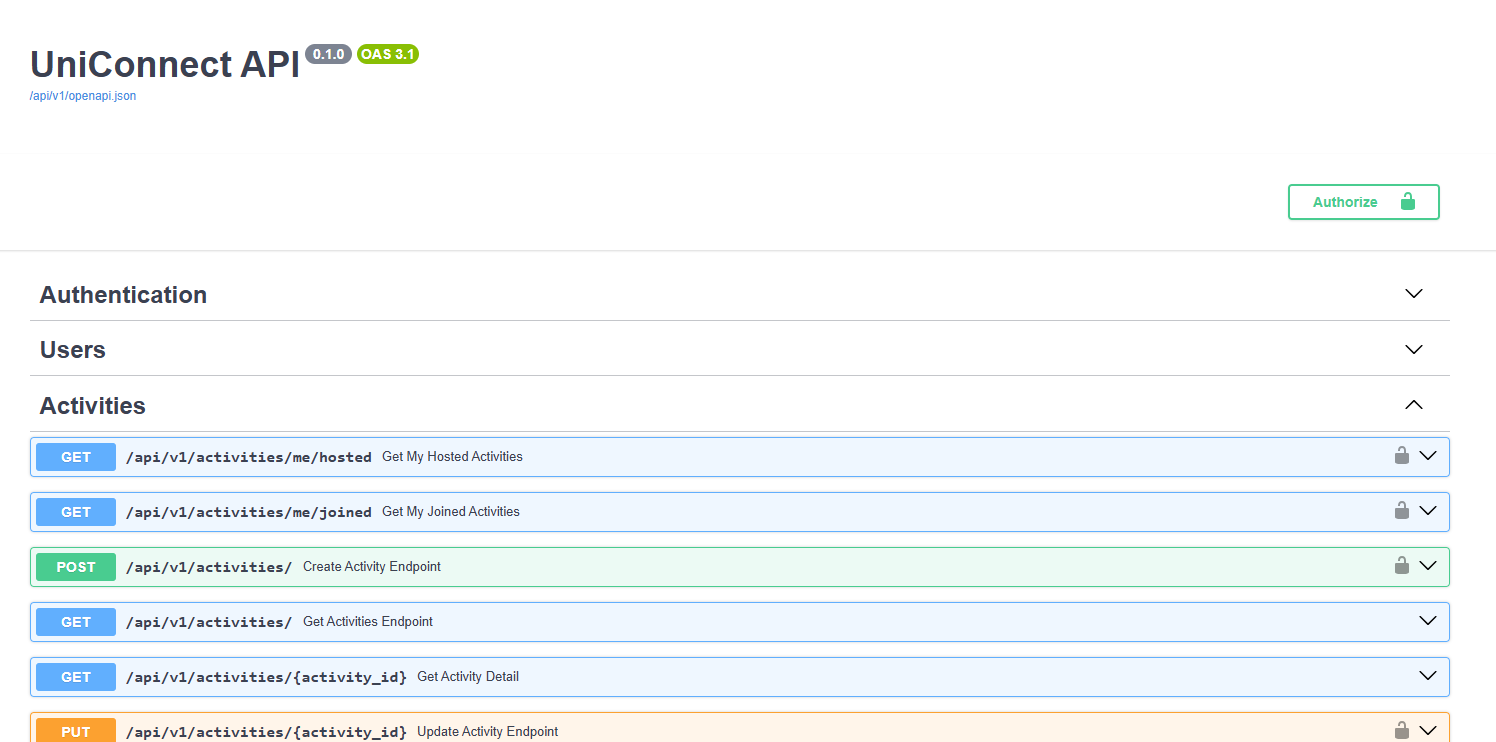
\includegraphics[width=0.85\textwidth]{Images/swagger.png} 
    \caption{Swagger UI của đề tài}
    \label{fig:swagger}
\end{figure}

\subsubsection{Đóng gói ứng dụng với Docker}

Để đảm bảo hệ thống vận hành ổn định trên mọi môi trường, dự án được đóng gói bằng công nghệ Docker. Toàn bộ dịch vụ bao gồm mã nguồn Backend và cơ sở dữ liệu PostgreSQL (tích hợp PostGIS/pgvector) được điều phối thông qua tệp cấu hình \texttt{docker-compose.yml}.

\begin{mycode}[Docker-Compose Orchestration]{}
services:
  # 1. Server Backend
  backend:
    build: .
    container_name: uniconnect_api
    ports:
      - "8000:8000"
    env_file:
      - .env
    volumes:
      - .:/app
    depends_on:
      db:
        condition: service_healthy
      redis:
        condition: service_started

  # 2. Database (Đã tích hợp PostGIS + pgvector)
  db:
    build: 
      context: .
      dockerfile: Dockerfile.db
    container_name: uniconnect_db
    environment:
      - POSTGRES_USER=\${DB_USER}
      - POSTGRES_PASSWORD=\${DB_PASSWORD}
      - POSTGRES_DB=\${DB_NAME}
    ports:
      - "5432:5432"
    volumes:
      - postgres_data:/var/lib/postgresql/data
    healthcheck:
      test: ["CMD-SHELL", "pg_isready -U \${DB_USER} -d \${DB_NAME}"]
      interval: 5s   
      timeout: 5s   
      retries: 5
      
  # 3. Redis
  redis:
    image: redis:alpine
    container_name: uniconnect_redis
    ports:
      - "6379:6379" 
    volumes:
      - redis_data:/data

volumes:
  postgres_data:
  redis_data:
\end{mycode}

Việc sử dụng Docker giúp rút ngắn thời gian triển khai và đảm bảo các thành phần mở rộng của cơ sở dữ liệu luôn sẵn sàng mà không cần cài đặt thủ công.

\subsection{Kết luận chương}

Chương này đã khái quát quá trình hiện thực hóa các thành phần cốt lõi của Backend, từ cấu trúc tổ chức mã nguồn đến các tính năng then chốt về xử lý dữ liệu không gian, tìm kiếm ngữ nghĩa và triển khai hệ thống. Đây là nền tảng vững chắc để phát triển giao diện người dùng và tích hợp các dịch vụ thông minh trong giai đoạn tiếp theo.



\section{Hiện thực giao diện người dùng (Frontend)}

\subsection{Công nghệ và kiến trúc giao diện}
Giao diện người dùng của nền tảng UniConnect được xây dựng theo mô hình ứng dụng đơn trang (Single Page Application - SPA) hiện đại, đáp ứng các tiêu chuẩn về tính tương tác thời gian thực, độ mượt mà và khả năng thích ứng đa nền tảng (Responsive Web Design).

Các công nghệ và thư viện chủ chốt được ứng dụng trong phân hệ Frontend bao gồm:
\begin{itemize}
    \item \textbf{Thư viện lõi React 18 kết hợp TypeScript:} Tận dụng tính năng Concurrent Rendering, phân tách mã theo cấu trúc Component hóa tái sử dụng cao, đảm bảo tính chặt chẽ về mặt kiểu dữ liệu và giảm thiểu tối đa các lỗi lúc thực thi (runtime errors).
    \item \textbf{Công cụ đóng gói Vite:} Cung cấp môi trường phát triển với tốc độ biên dịch cực nhanh dựa trên ES Modules nguyên bản (Native ESM), tối ưu hóa kích thước gói phát hành (bundle size) và hỗ trợ cơ chế tải động theo trang (Lazy Loading kết hợp React Suspense).
    \item \textbf{Kiến trúc điều hướng và Quản lý trạng thái:} Sử dụng \texttt{react-router-dom} (v6) để thiết lập luồng điều hướng SPA mượt mà không cần tải lại trang. Trạng thái xác thực phiên làm việc của người dùng (Authentication Context) và hệ thống thông báo trạng thái tức thời (Toast Notification Context) được quản lý tập trung thông qua React Context API.
    \item \textbf{Giao tiếp mạng bất đồng bộ:} Thư viện Axios được cấu hình với các Interceptor tự động gắn Access Token (Bearer JWT) vào tiêu đề mọi yêu cầu và chủ động xử lý các mã lỗi HTTP chuẩn mực (401 Unauthorized, 403 Forbidden, 422 Validation Error).
    \item \textbf{Thiết kế giao diện hiện đại (Styling \& Design System):} Kết hợp các biến CSS Tokens toàn cục cùng hệ thống lưới linh hoạt (Flexbox và CSS Grid), mang lại khả năng hiển thị đồng nhất, hỗ trợ tốt chế độ sáng/tối (Dark Mode) và thân thiện với thiết bị di động (Mobile-first).
    \item \textbf{Bộ biểu tượng Lucide Icons \& Xử lý Markdown:} Tích hợp bộ icon vector chuẩn hóa đồng bộ nhận diện trực quan cùng thư viện \texttt{react-markdown} kết hợp \texttt{remark-gfm} để hiển thị nội dung định dạng phong phú từ các bài đăng và câu trả lời thông minh của Trợ lý AI.
\end{itemize}

\subsection{Chi tiết các màn hình chức năng cốt lõi}
Dưới đây là chi tiết các màn hình chức năng tiêu biểu đã được hiện thực hóa và vận hành ổn định trên hệ thống:

\subsubsection{Màn hình Bảng điều khiển và Khám phá Hoạt động (Student Dashboard)}
Giao diện trung tâm cho phép sinh viên theo dõi toàn bộ các sự kiện học đường và phong trào tình nguyện sắp diễn ra. Hệ thống cung cấp bộ lọc đa tiêu chí (học thuật, thể thao, tình nguyện, CTXH), thanh tìm kiếm thông minh và các thẻ hoạt động trực quan hiển thị đầy đủ thông tin thời gian, địa điểm cũng như số ngày CTXH tích lũy.

\begin{figure}[H]
    \centering
    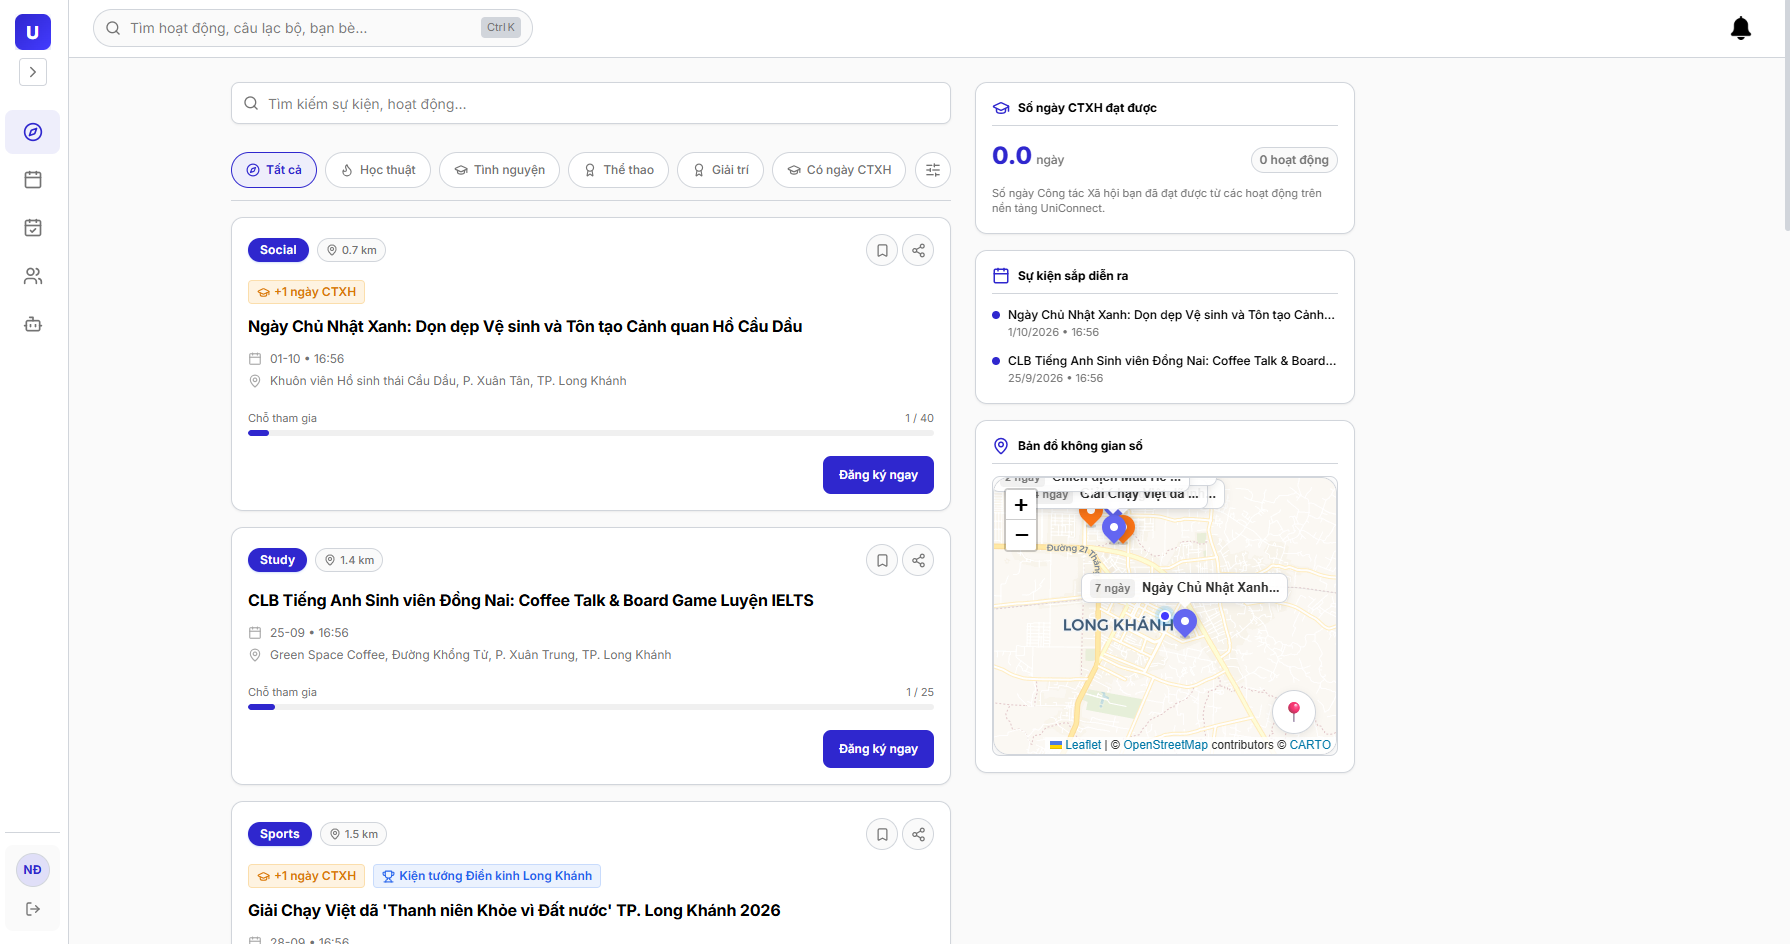
\includegraphics[width=0.68\textwidth]{Images/ui-dashboard.png}
    \caption{Giao diện Bảng điều khiển sinh viên và khám phá các hoạt động ngoại khóa}
    \label{fig:ui_dashboard}
\end{figure}

\subsubsection{Màn hình Chi tiết Hoạt động và Đăng ký tham gia (Activity Details)}
Cung cấp đầy đủ thông tin chi tiết về sự kiện: thời gian diễn ra, địa điểm tập trung, câu lạc bộ hoặc đơn vị tổ chức, số lượng suất tham gia còn lại và danh sách sinh viên tham dự. Hệ thống tự động đối soát lịch trình cá nhân theo thời gian thực để cảnh báo khả năng xung đột thời gian và cung cấp nút đăng ký tham gia trực tiếp.

\begin{figure}[H]
    \centering
    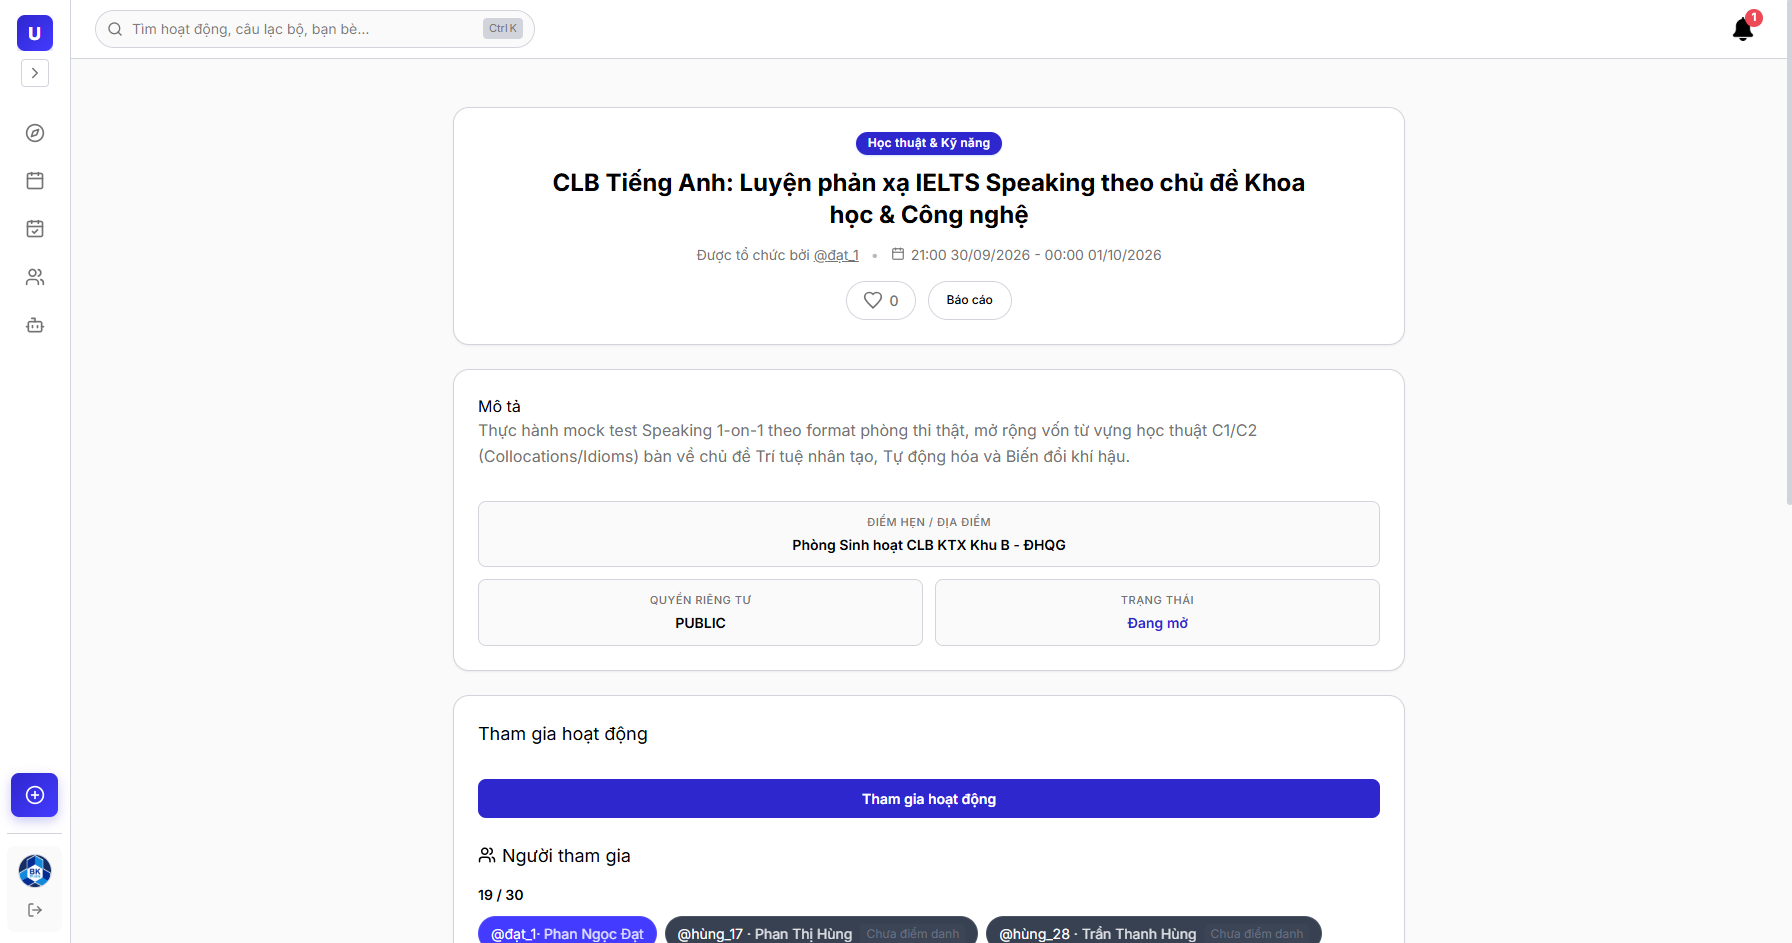
\includegraphics[width=0.68\textwidth]{Images/ui-activity-detail.png}
    \caption{Giao diện Chi tiết hoạt động và đối soát lịch trình đăng ký}
    \label{fig:ui_activity_detail}
\end{figure}

\clearpage
\subsubsection{Màn hình Khởi tạo và Thiết lập Hoạt động (Create Activity)}
Giao diện dành cho ban tổ chức và ban chủ nhiệm các câu lạc bộ để thiết lập sự kiện mới. Biểu mẫu hỗ trợ cấu hình toàn diện các thông số: tiêu đề, mô tả chi tiết, danh mục, thời gian diễn ra, địa điểm tổ chức trên bản đồ, số lượng người tham gia tối đa, định mức ngày CTXH và tùy chọn phê duyệt đơn tham gia.

\begin{figure}[H]
    \centering
    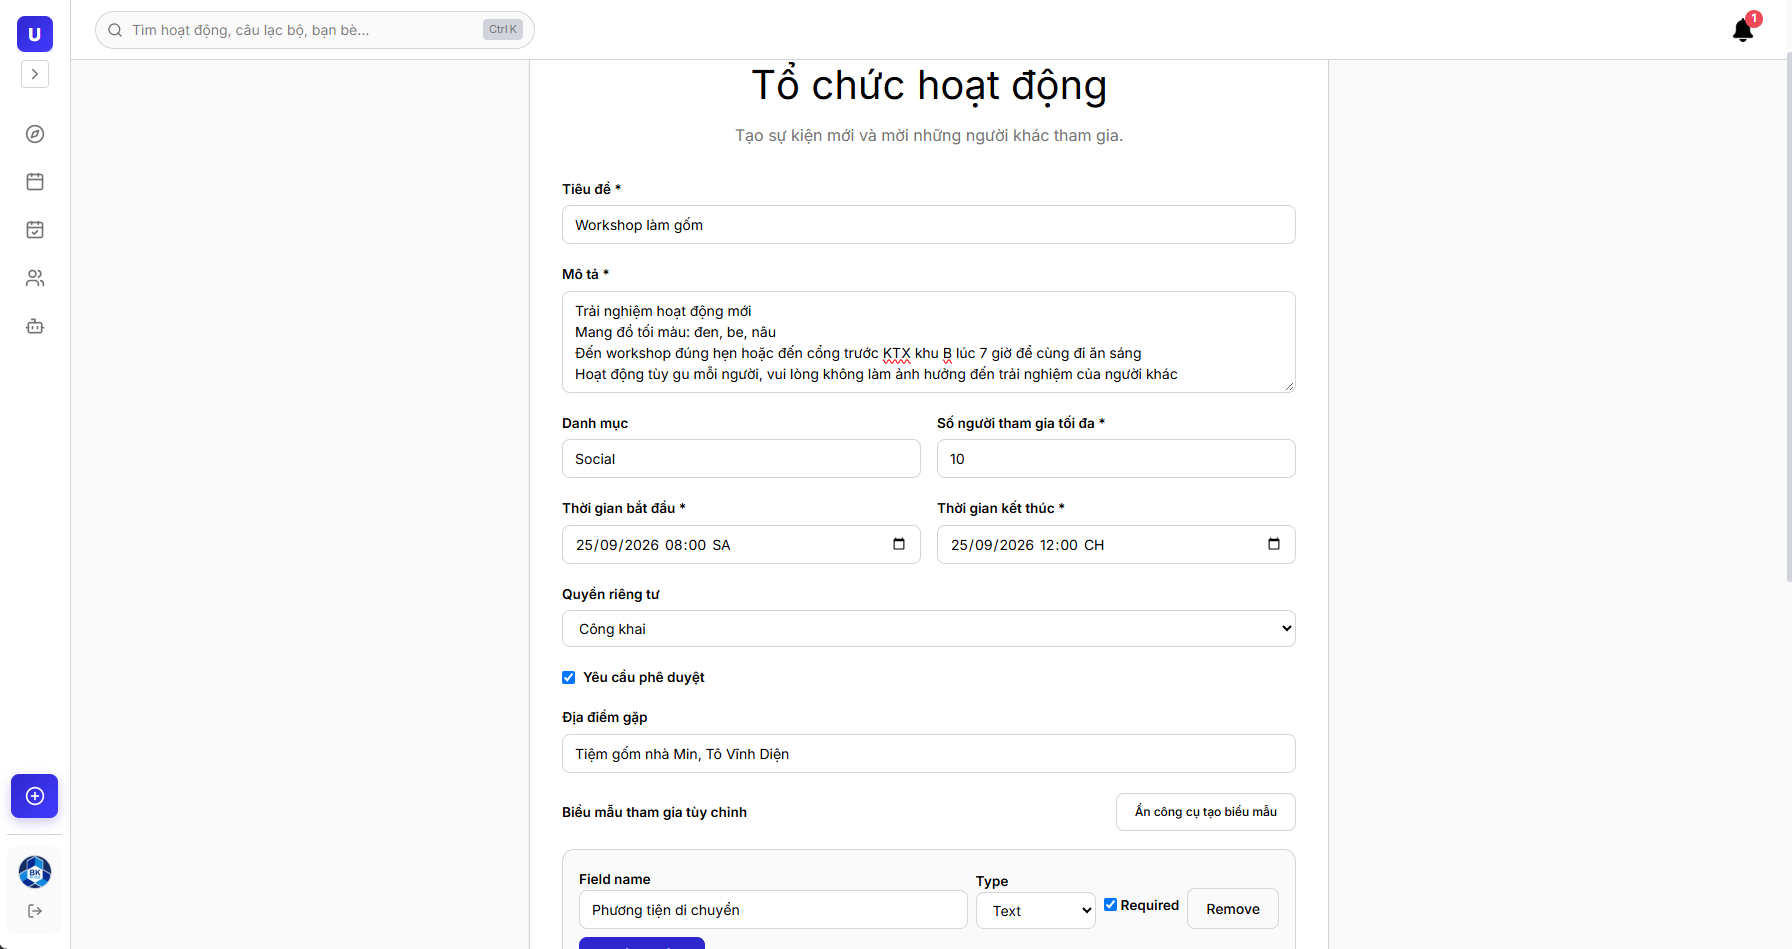
\includegraphics[width=0.68\textwidth]{Images/ui-tao-hoat-dong.png}
    \caption{Giao diện Khởi tạo và thiết lập thông số hoạt động phong trào mới}
    \label{fig:ui_tao_hoat_dong}
\end{figure}

\subsubsection{Màn hình Lịch Thông minh và Quản lý Lịch trình (Smart Calendar Schedule)}
Hiển thị trực quan lịch trình cá nhân của sinh viên theo các chế độ xem linh hoạt (tuần/tháng), tích hợp đồng thời các khung giờ bận cố định (thời khóa biểu học tập) cùng các sự kiện ngoại khóa đã xác nhận tham gia. Hệ thống hỗ trợ chức năng xuất nhanh tệp chuẩn \texttt{.ics} để đồng bộ lịch trình hai chiều vào Google Calendar hoặc Apple Calendar.

\begin{figure}[H]
    \centering
    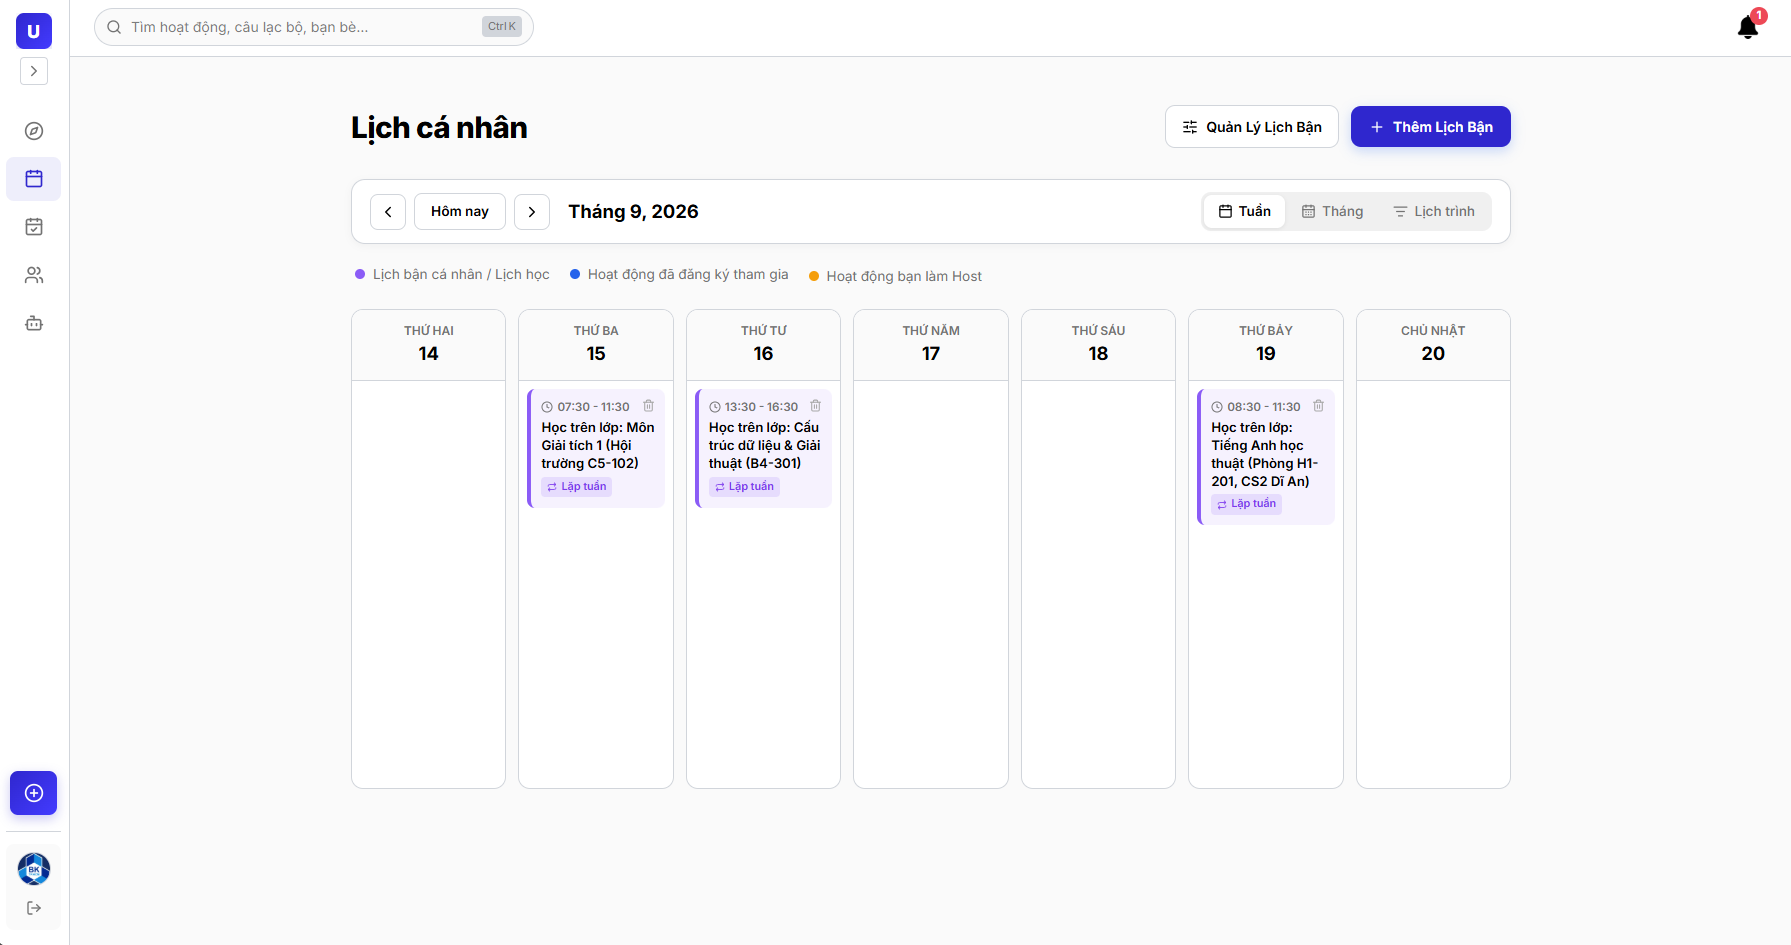
\includegraphics[width=0.68\textwidth]{Images/ui-lich-ca-nhan.png}
    \caption{Giao diện Lịch thông minh và quản lý khung giờ bận cá nhân}
    \label{fig:ui_smart_calendar}
\end{figure}

\clearpage
\subsubsection{Màn hình Trợ lý Học đường AI Thông minh (AI Assistant Chatbot)}
Giao diện tương tác trò chuyện với Trợ lý AI UniConnect. Người dùng có thể đặt câu hỏi tự nhiên để nhờ tìm kiếm sự kiện phù hợp, đối soát lịch bận cá nhân hoặc tra cứu các câu lạc bộ học đường. Phản hồi của Trợ lý AI cung cấp đầy đủ thông tin súc tích kèm theo các đường dẫn (hyperlink) điều hướng trực tiếp đến trang chi tiết hoạt động và câu lạc bộ tương ứng.

\begin{figure}[H]
    \centering
    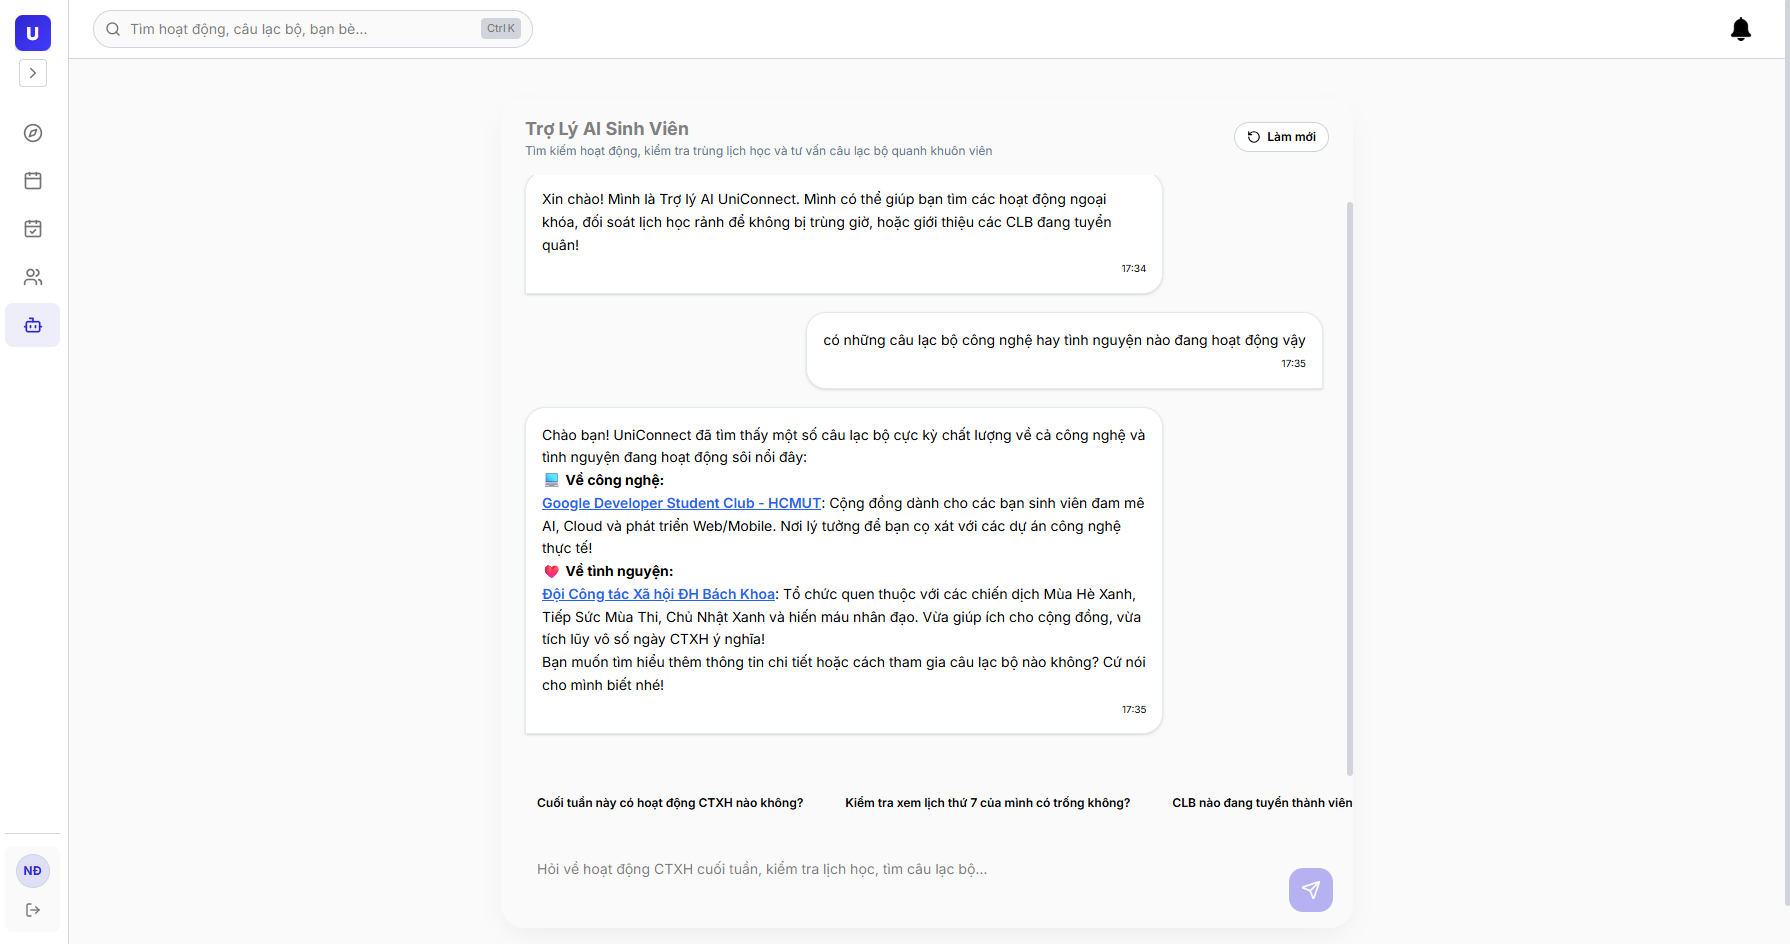
\includegraphics[width=0.68\textwidth]{Images/ui-chatbot.png}
    \caption{Giao diện Trợ lý học đường AI giải đáp thông tin và gợi ý hoạt động}
    \label{fig:ui_chatbot}
\end{figure}

\subsubsection{Màn hình Cộng đồng và Câu lạc bộ Sinh viên (Student Communities \& Clubs)}
Không gian kết nối và sinh hoạt của các câu lạc bộ, đội nhóm phong trào trong toàn trường. Người dùng có thể tra cứu thông tin giới thiệu, mục tiêu hoạt động, số lượng thành viên của từng CLB và nộp đơn đăng ký tham gia cộng đồng.

\begin{figure}[H]
    \centering
    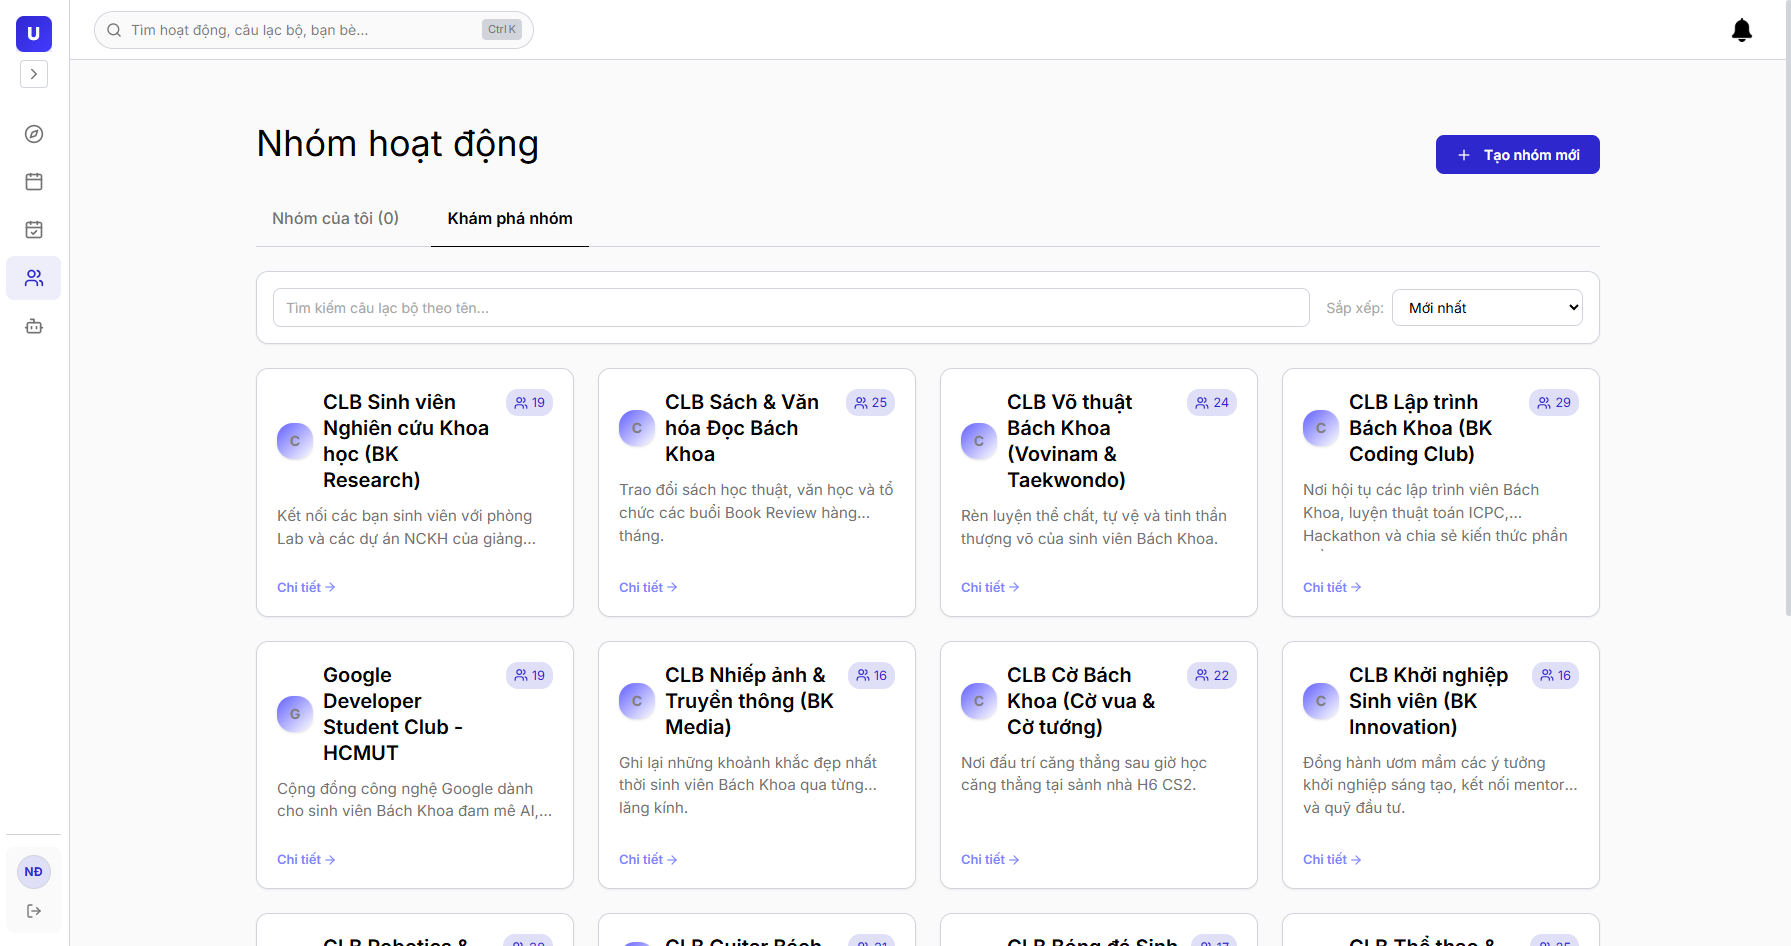
\includegraphics[width=0.68\textwidth]{Images/ui-nhom.png}
    \caption{Giao diện Danh sách và thông tin các câu lạc bộ, đội nhóm học đường}
    \label{fig:ui_nhom}
\end{figure}

\clearpage
\subsubsection{Màn hình Hồ sơ Cá nhân và Vinh danh Thành tích (Gamification Profile)}
Không gian vinh danh nỗ lực tham gia hoạt động của sinh viên: hiển thị tổng số ngày Công tác Xã hội (CTXH) tích lũy, cấp bậc thứ hạng sinh viên, tủ trưng bày bộ sưu tập danh hiệu Trophy đã mở khóa và lịch sử chi tiết các sự kiện sinh viên đã tham gia.

\begin{figure}[H]
    \centering
    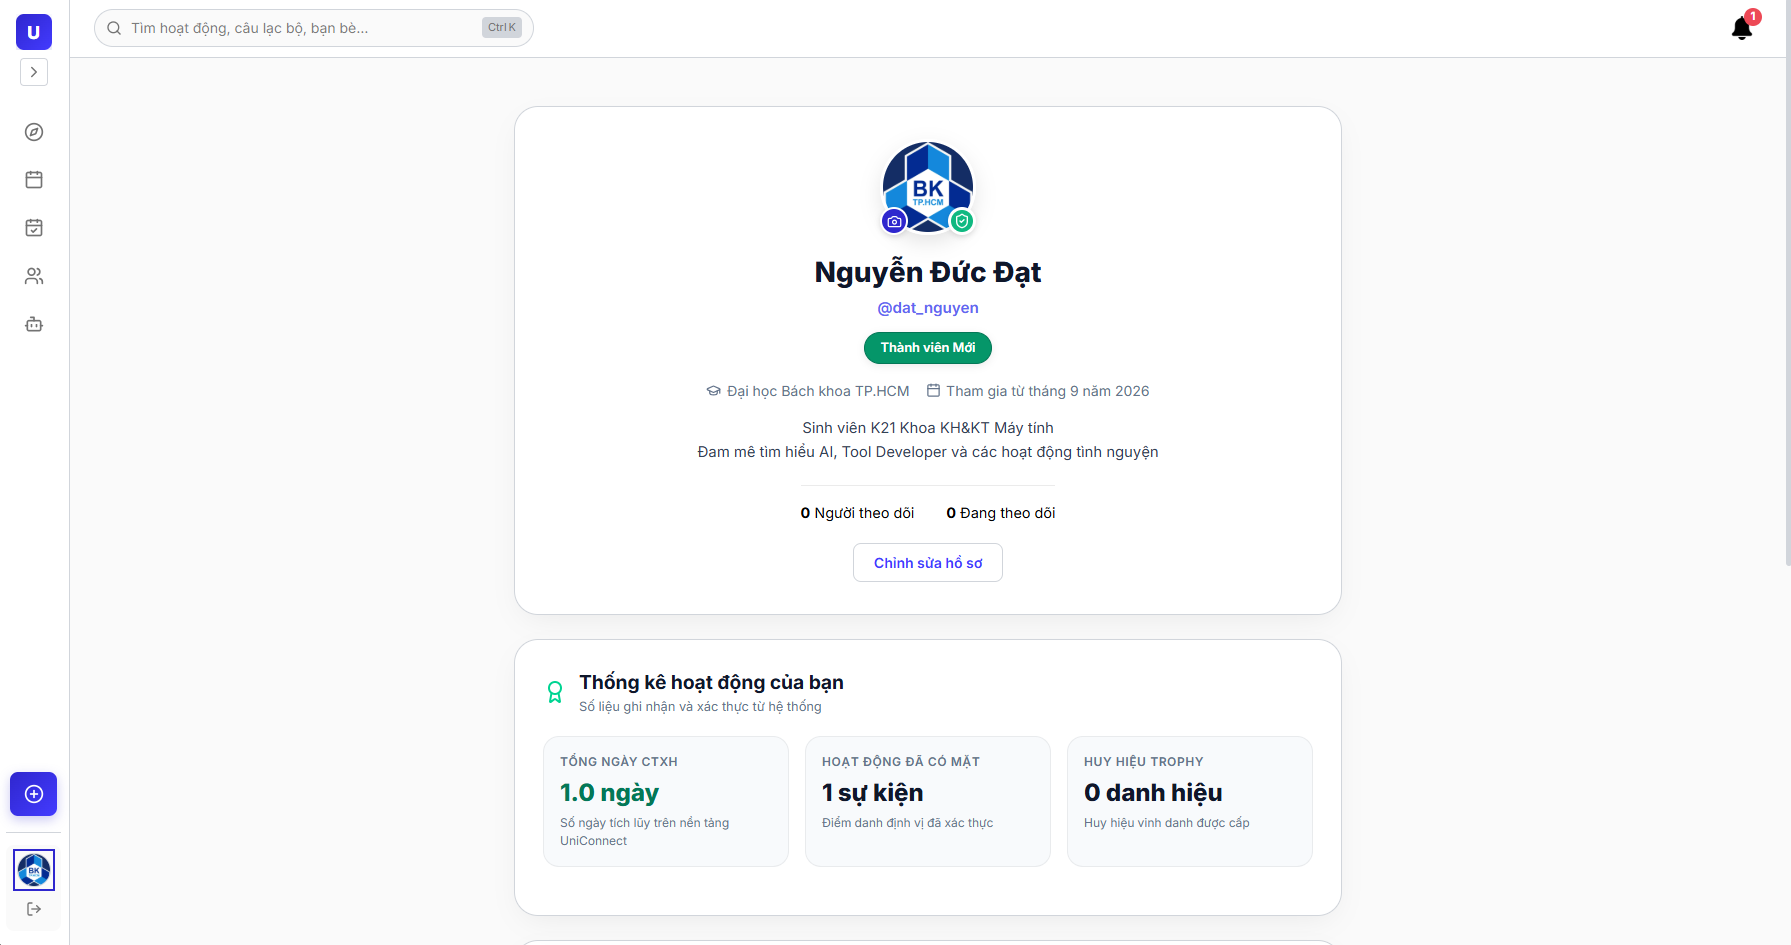
\includegraphics[width=0.68\textwidth]{Images/ui-profile.png}
    \caption{Giao diện Hồ sơ cá nhân, tiến trình tích lũy CTXH và danh hiệu Trophy}
    \label{fig:ui_profile}
\end{figure}

\subsubsection{Màn hình Giấy xác nhận Tham gia Hoạt động (Activity Participation Certificate)}
Biểu mẫu hành chính điện tử công nhận sự tham gia của sinh viên sau khi hoàn thành hoạt động. Giấy xác nhận được trình bày theo thể thức văn bản chuẩn mực, bao gồm tên đơn vị tổ chức, tên hoạt động, số ngày CTXH ghi nhận, mã tra cứu xác thực và nút tải trực tiếp tệp tin PDF về máy phục vụ cho việc nộp minh chứng điểm rèn luyện.

\begin{figure}[H]
    \centering
    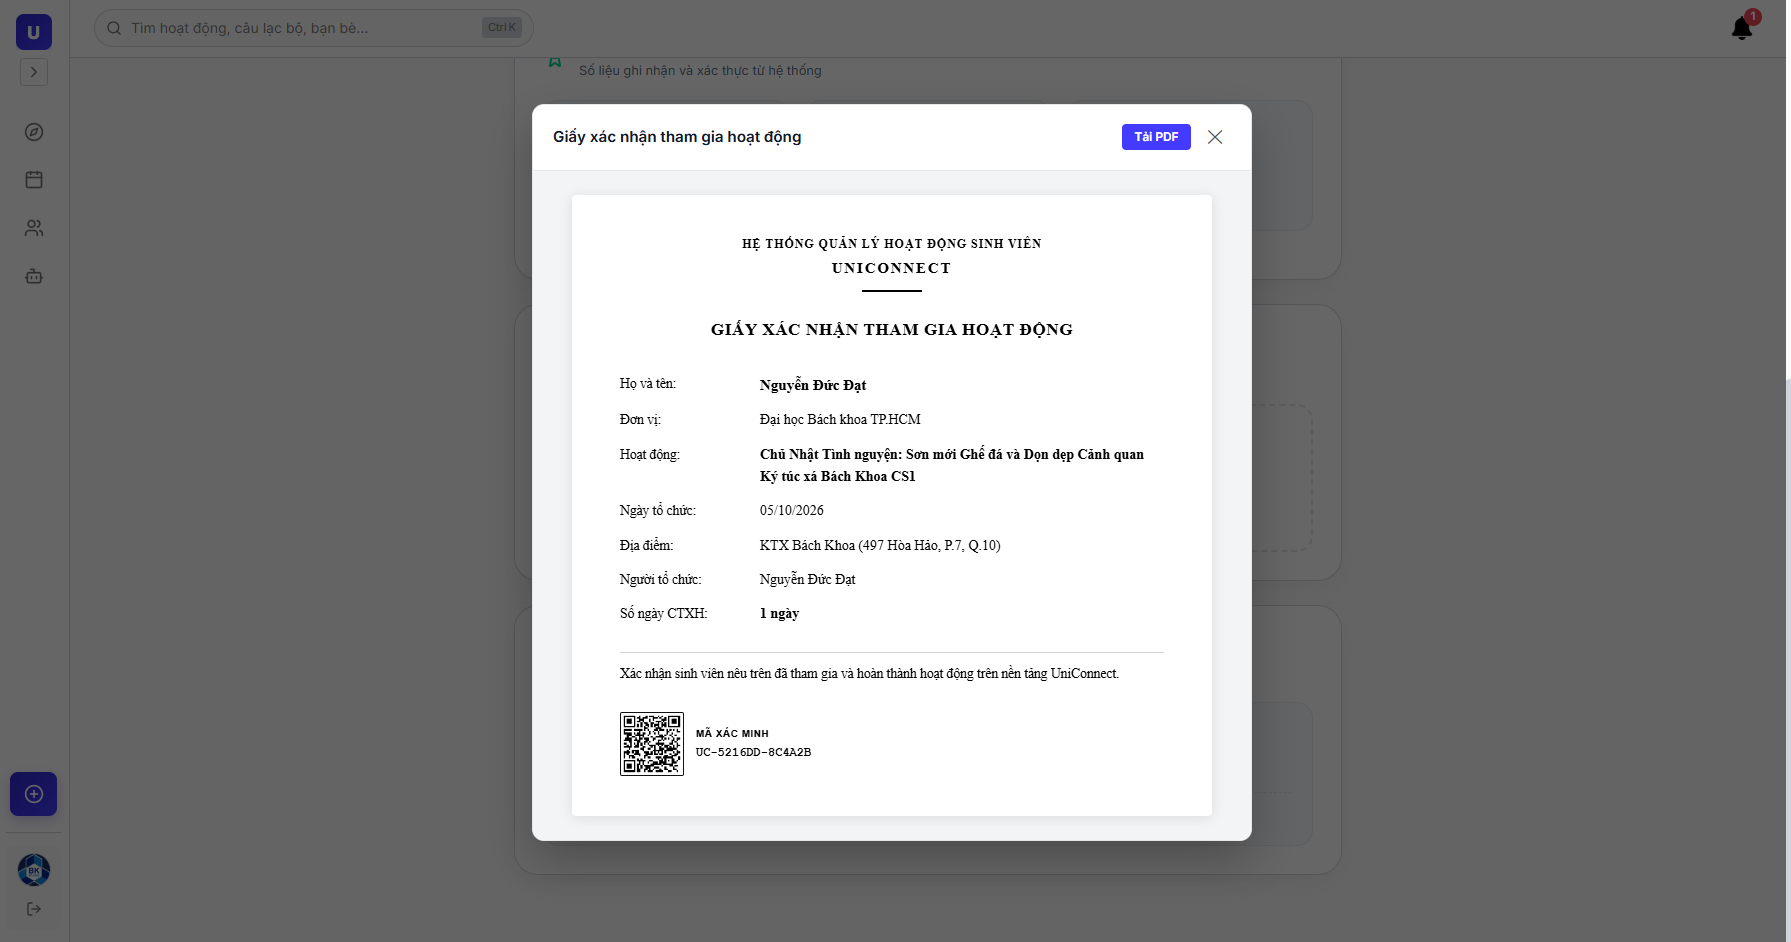
\includegraphics[width=0.68\textwidth]{Images/ui-giay-xac-nhan-tham-gia.png}
    \caption{Giao diện Giấy xác nhận tham gia hoạt động điện tử chuẩn hành chính}
    \label{fig:ui_certificate_modal}
\end{figure}

\subsection{Kết luận chương}
Chương này đã trình bày toàn diện quá trình hiện thực hóa giao diện người dùng Frontend của nền tảng UniConnect. Bằng việc ứng dụng React 18, TypeScript, Vite và ngôn ngữ thiết kế chuẩn mực, hệ thống mang lại trải nghiệm tương tác trực quan, mượt mà và thích ứng linh hoạt đa thiết bị. Toàn bộ 8 màn hình chức năng cốt lõi đã được hoàn thiện chỉn chu, tối ưu hóa kích thước gói tải, bảo đảm tính toàn vẹn dữ liệu và sẵn sàng phục vụ nhu cầu phong trào thực tế của sinh viên.


\section{Hiện thực hệ thống trợ lý AI và Gợi ý hoạt động}

Hệ thống Trợ lý AI của UniConnect được xây dựng dựa trên kiến trúc RAG (Retrieval-Augmented Generation) kết hợp mô hình suy luận ReAct Agent và phân tích ngữ cảnh người dùng theo thời gian thực. Khác với các chatbot hỏi đáp thông thường, Trợ lý AI trong UniConnect có khả năng thấu hiểu lịch trình cá nhân, sở thích của người dùng và dữ liệu bản đồ hoạt động học đường để đưa ra các gợi ý chính xác và có thể thực thi được.

\subsection{Kiến trúc Hybrid Context (Ngữ cảnh hỗn hợp)}

Để sinh câu trả lời và đưa ra gợi ý chất lượng, hệ thống tổng hợp ngữ cảnh từ ba nguồn dữ liệu chính:
\begin{enumerate}
    \item \textbf{Campus Events \& Rules (Tri thức hoạt động):} Thông tin chi tiết về các sự kiện, tiêu chí ngày CTXH, địa điểm tổ chức và quy định công nhận ngày CTXH từ bảng \texttt{activities} thông qua truy vấn tìm kiếm Vector \textit{pgvector}.

    \item \textbf{Personal Schedule \& Interests (Lịch trình và Sở thích):} Dữ liệu thời khóa biểu, khoảng thời gian bận cố định từ bảng \texttt{user\_busy\_slots}, lịch trình tham gia sự kiện đã duyệt trong \texttt{join\_requests} và danh sách từ khóa sở thích (\texttt{interests}) trong hồ sơ người dùng.
    
    \item \textbf{Social Context (Mạng lưới quan hệ):} Các hoạt động có sự tham gia của các Nhóm sinh viên mà người dùng đang là thành viên hoặc những người dùng mà người dùng đang theo dõi (\texttt{user\_follows}), giúp nắm bắt xu hướng phong trào trong cộng đồng.
\end{enumerate}

\subsection{Hiện thực luồng xử lý gợi ý hoạt động cá nhân hóa}

Khi người dùng mở giao diện Bản đồ hoặc yêu cầu Trợ lý AI gợi ý hoạt động, hệ thống thực hiện quy trình xử lý 4 giai đoạn:
\begin{enumerate}
    \item \textbf{Giai đoạn 1 -- Khai thác Vector sở thích:} Hệ thống tính toán vector đại diện cho sở thích của người dùng dựa trên lịch sử hoạt động đã tham gia và danh mục quan tâm trong hồ sơ cá nhân.
    
    \item \textbf{Giai đoạn 2 -- Lọc không gian (Spatial Filtering):} Sử dụng hàm \texttt{ST\_DWithin} của PostGIS để lọc ra các hoạt động đang hoặc sắp diễn ra trong bán kính lân cận khuôn viên trường.

    \item \textbf{Giai đoạn 3 -- Kiểm tra khả dụng thời gian (Calendar Conflict Filtering):} Hệ thống đối soát khung giờ bắt đầu/kết thúc của các hoạt động tiềm năng với bảng \texttt{user\_busy\_slots} và các sự kiện đã đăng ký trong \texttt{join\_requests}. Những sự kiện bị trùng với lịch học cố định hoặc sự kiện đã xác nhận tham gia sẽ được gắn cờ cảnh báo (\texttt{hard\_conflict}) để tránh gợi ý người dùng tham gia vào khung giờ bận.

    \item \textbf{Giai đoạn 4 -- Xếp hạng và Gợi ý (Ranking):} Tổng hợp điểm tương đồng ngữ nghĩa (Cosine Similarity), khoảng cách địa lý và độ ưu tiên từ mạng lưới bạn bè để trả về danh sách Top-K hoạt động tối ưu nhất cho người dùng.
\end{enumerate}

\subsection{Quy trình vận hành RAG Pipeline của Trợ lý AI}

Khi người dùng đặt câu hỏi tự nhiên qua khung chat (ví dụ: \textit{"Thứ Bảy này tôi có thời gian trống vào buổi sáng, có hoạt động tình nguyện nào quanh khu vực trường cấp ngày CTXH không?"}), quy trình xử lý diễn ra như sau:
\begin{enumerate}
    \item \textbf{Text Embedding:} Câu hỏi của người dùng được chuyển đổi thành vector truy vấn 768 chiều thông qua mô hình Gemini Embedding 001 (\texttt{gemini-embedding-001}).
    \item \textbf{Vector Distance Query (pgvector):} Hệ thống thực thi truy vấn tính toán khoảng cách Cosine trực tiếp trên cột \texttt{embedding} (\texttt{Vector(768)}) của bảng \texttt{activities} thông qua toán tử khoảng cách \texttt{cosine\_distance} của thư viện \texttt{pgvector-python}, kết hợp mệnh đề lọc theo trạng thái sự kiện hợp lệ để trích xuất các hoạt động tương đồng nhất.
    \item \textbf{Dynamic Context Injection:} Đóng gói câu hỏi gốc cùng danh sách sự kiện tương đồng trích xuất được và thông tin thời khóa biểu cá nhân của người dùng thành Prompt ngữ cảnh chuẩn hóa.
    \item \textbf{LLM Generation:} Mô hình ngôn ngữ lớn phân tích ngữ cảnh tổng hợp và sinh câu trả lời tư vấn lịch trình tự nhiên, trực quan kèm đường dẫn điều hướng tới trang chi tiết sự kiện trên bản đồ.
\end{enumerate}

\textbf{Ghi chú kỹ thuật về lưu trữ và chỉ mục vector:} Vector đặc trưng ngữ nghĩa được lưu tại cột \texttt{embedding} kiểu dữ liệu \texttt{Vector(768)} của bảng \texttt{activities}. Với quy mô dữ liệu học đường hiện tại, hệ thống thực hiện đối soát khoảng cách Cosine trực tiếp (Exact Nearest Neighbor). Việc cấu hình chỉ mục xấp xỉ đồ thị HNSW (Hierarchical Navigable Small World) trên cơ sở dữ liệu được xác định là giải pháp mở rộng quy mô khi hệ sinh thái sự kiện mở rộng vượt ngưỡng hàng chục nghìn bản ghi.


\include{Sections/9-Kiem-thu-va-danh-gia}

\section{Kết luận và hướng phát triển}

\subsection{Kết quả đạt được}
Sau thời gian nghiên cứu, phân tích kiến trúc và hiện thực hóa toàn diện giải pháp, tác giả đề tài đã hoàn thành tốt các mục tiêu đề ra cho nền tảng \textbf{UniConnect: Hệ thống kết nối hoạt động sinh viên dựa trên bản đồ số và trợ lý ảo thông minh}. Các kết quả cụ thể đạt được bao gồm:

\begin{itemize}[leftmargin=*]
    \item \textbf{Xây dựng hoàn chỉnh nền tảng Web Fullstack hiện đại:} Phát triển giao diện người dùng dựa trên thư viện React 18, Vite và TypeScript kết hợp hệ thống thiết kế giao diện chuẩn mực (Lucide Design System). Ứng dụng thành công kỹ thuật phân tách mã nguồn động (Code-splitting) thông qua \texttt{React.lazy()} và chia nhỏ gói mã nguồn (Chunking Strategy), giúp giảm tới 72.0\% kích thước gói tài nguyên JavaScript ban đầu (từ 842.80~kB xuống 236.02~kB), rút ngắn thời gian tải trang ban đầu còn $\approx$ 1.3 giây trên hạ tầng mạng di động học đường.
    
    \item \textbf{Bản đồ số học đường và Quản trị hoạt động - Nhóm sinh viên:} Tích hợp thành công bản đồ khuôn viên trường bằng Leaflet và mở rộng dữ liệu không gian PostGIS (chuẩn hệ quy chiếu EPSG:4326). Hệ thống hỗ trợ tìm kiếm, lọc hoạt động theo bán kính vị trí thực tế, quản lý toàn bộ vòng đời hoạt động phong trào và thiết lập cơ chế liên kết Đồng tổ chức (Co-hosting) giữa các Nhóm sinh viên với sự phân tách quyền hạn ủy nhiệm rõ ràng (\texttt{can\_open\_checkin} và \texttt{can\_manage\_activity}).
    
    \item \textbf{Hệ thống Điểm danh chống gian lận đa chế độ:} Hiện thực hóa thành công kiến trúc điểm danh bảo mật: mã QR xoay động 30 giây được ký số bảo vệ bằng thuật toán HMAC-SHA256 kết hợp hàng rào địa lý GPS Geofencing (ràng buộc khoảng cách không gian $d \le 100$m và ngưỡng sai số phần cứng $acc \le 100$m), tích hợp giao diện hiệu ứng sóng Radar quét vệ tinh tự động trên thiết bị người dùng.
    
    \item \textbf{Lịch cá nhân thông minh \& Khử xung đột tự động:} Xây dựng phân hệ Smart Calendar hỗ trợ quản trị thời gian biểu sinh viên, tự động nhận diện xung đột thời gian cứng/mềm theo vị từ khoảng nửa mở $[start, end)$, hỗ trợ lịch bận lặp lại định kỳ hàng tuần kèm cơ chế bỏ qua ngoại lệ ngày nghỉ (vacation suppression), và cho phép đồng bộ hóa dữ liệu ra các ứng dụng lịch phổ biến chuẩn quốc tế \texttt{.ics}.
    
    \item \textbf{Trợ lý Trí tuệ nhân tạo học đường (RAG AI Assistant):} Tích hợp mô hình ngôn ngữ lớn kết hợp tìm kiếm ngữ nghĩa tăng cường (Retrieval-Augmented Generation) thông qua mở rộng vector hóa \texttt{pgvector} (vector 768 chiều). Trợ lý AI hỗ trợ cơ chế gọi hàm (Function Calling) linh hoạt để tự động truy vấn hoạt động và thông tin nhóm sinh viên, bảo đảm nghiêm ngặt quyền riêng tư cá nhân và duy trì cơ chế hồi quy tất định (Deterministic Fallback) ngay cả khi dịch vụ AI ngoại tuyến.
    
    \item \textbf{Chứng nhận số trực tuyến \& Cơ chế Trò chơi hóa (Gamification):} Tự động hóa quá trình tích lũy ngày Công tác Xã hội (CTXH) sau khi xác nhận điểm danh hợp lệ; thiết lập chu trình quản lý danh hiệu Gamification chặt chẽ với cơ chế chốt điểm danh (Finalize Attendance), kiểm tra điều kiện túc số (Quorum $\ge 10$) và thẩm định phê duyệt từ Quản trị viên trước khi chính thức trao tặng Trophy cho sinh viên; cung cấp chức năng xuất Giấy chứng nhận điện tử chuẩn in ấn PDF A4 kèm mã tra cứu và cổng kiểm chứng tính nguyên bản công khai tại \texttt{/verify-certificate}.
    
    \item \textbf{Bảng điều khiển Quản trị toàn diện \& Xuất dữ liệu chuẩn hóa:} Xây dựng Admin Command Center hỗ trợ giám sát các chỉ số KPI hoạt động theo công thức tăng trưởng xác định, cơ chế kiểm duyệt nội dung vi phạm bằng giao dịch nguyên tử (Atomic transaction) kèm ghi vết Admin Audit Log, và cơ chế truyền dòng (streaming) xuất danh sách sinh viên định dạng CSV UTF-8 BOM chống lỗi font tiếng Việt.
    
    \item \textbf{Hạ tầng đóng gói Deployment-Ready \& Bảo đảm chất lượng tham chiếu IEEE 829:} Đóng gói hệ thống theo kiến trúc Multi-stage Docker Container, thực thi dưới người dùng bảo mật không đặc quyền (\texttt{appuser:1001}), Nginx reverse proxy bảo vệ phân vùng tin cậy mạng (trust boundary), và vượt qua 100\% bộ kiểm thử tự động toàn diện tham chiếu các nguyên tắc tài liệu kiểm thử theo tiêu chuẩn phần mềm IEEE 829\cite{ieee829test} bao gồm \textbf{94 ca kiểm thử tự động Backend} (thuộc 14 test suites) cùng quy trình đóng gói Frontend tối ưu hóa không phát sinh lỗi TypeScript hay bundling.
\end{itemize}

\subsection{Hạn chế còn tồn tại}
Bên cạnh các kết quả tích cực đã đạt được, hệ thống vẫn còn một số mặt hạn chế cần tiếp tục hoàn thiện:

\begin{enumerate}[leftmargin=*, noitemsep]
    \item \textbf{Hạn chế về nền tảng ứng dụng di động (Mobile Web vs Native App):} Hệ thống hiện vận hành trên nền tảng Web đáp ứng (Responsive Web). Mặc dù giao diện hiển thị tối ưu trên màn hình điện thoại, ứng dụng web chưa thể khai thác sâu các tính năng cấp hệ điều hành như cảm biến camera quét mã QR phần cứng siêu tốc hay dịch vụ thông báo đẩy nền (Background Push Notifications).
    \item \textbf{Phụ thuộc độ trễ dịch vụ Trí tuệ nhân tạo đám mây:} Trợ lý AI hiện đang sử dụng dịch vụ đám mây (Google Gemini API), do đó thời gian xử lý và phản hồi đối với các câu hỏi phức tạp phụ thuộc vào đường truyền Internet quốc tế và giới hạn tần suất (rate limits) của nhà cung cấp.
    \item \textbf{Sai số định vị GPS trong môi trường nhà kín (Indoor Multipath):} Tín hiệu định vị vệ tinh GPS có thể bị suy hao hoặc sai số tăng cao ($acc > 100$m) khi người dùng ở sâu bên trong các giảng đường lớn, tầng hầm hoặc phòng họp kín, đòi hỏi sự bổ trợ chính từ phương thức quét mã QR HMAC xoay động.
    \item \textbf{Phạm vi dữ liệu và tích hợp liên trường:} Hệ thống hiện thử nghiệm trong khuôn viên Đại học Bách Khoa, chưa tích hợp trực tiếp vào cổng đăng nhập tập trung (Single Sign-On VNU-ID) để liên thông chứng nhận ngày CTXH giữa các trường thành viên trong khối ĐHQG-HCM.
\end{enumerate}

\subsection{Định hướng phát triển trong tương lai}
Để nền tảng UniConnect phát triển toàn diện, bền vững và sẵn sàng phục vụ cộng đồng sinh viên trên quy mô lớn, tác giả định hướng mở rộng hệ thống theo hai nhóm phương diện chính:

\subsubsection{Phát triển và mở rộng tính năng ứng dụng}
\begin{itemize}[leftmargin=*, noitemsep]
    \item \textbf{Phát hành ứng dụng Native Mobile (Flutter / React Native):} Xây dựng ứng dụng di động độc lập đưa lên Google Play và Apple App Store, khai thác camera quét mã QR dưới 100ms, thông báo đẩy (FCM/APNs) và cơ chế chống giả lập GPS (Mock Location Detection).
    \item \textbf{Tích hợp xác thực sinh trắc học vào điểm danh:} Nghiên cứu bổ sung xác thực khuôn mặt (Face Verification) hoặc chuẩn WebAuthn/FIDO2 kết hợp mã QR HMAC và Geofencing, tạo chu trình xác minh 3 lớp chặt chẽ cho sự kiện quy mô lớn.
    \item \textbf{Mở rộng phân hệ Quản lý Tài chính và Kinh phí Nhóm:} Xây dựng mô-đun hỗ trợ Ban điều hành các nhóm sinh viên quản lý dự toán ngân sách hoạt động, ghi nhận đóng góp quỹ phong trào và minh bạch hóa các khoản thu/chi sự kiện.
    \item \textbf{Liên thông kết quả phong trào và Ngày CTXH toàn ĐHQG-HCM:} Mở rộng tích hợp hệ thống VNU-ID, cho phép sinh viên các trường thành viên đăng ký chéo hoạt động và đồng bộ kết quả ngày CTXH tự động về phòng Công tác Sinh viên.
\end{itemize}

\subsubsection{Nâng cấp hạ tầng kỹ thuật, bảo mật và trí tuệ nhân tạo}
\begin{itemize}[leftmargin=*, noitemsep]
    \item \textbf{Huấn luyện mô hình AI nội bộ (On-premise LLM):} Tinh chỉnh mô hình nguồn mở tiếng Việt (PhoGPT, Llama-3-Vietnamese) triển khai trên máy chủ Nhà trường, kết hợp tìm kiếm lai (Hybrid Search: BM25 + pgvector) nhằm giảm độ trễ dưới 500ms và bảo mật tuyệt đối dữ liệu học vụ.
    \item \textbf{Hỗ trợ hệ thống định vị hỗn hợp trong nhà (Indoor Positioning System):} Tích hợp thêm Bluetooth Low Energy (BLE Beacons) hoặc nhận diện mạng Wi-Fi giảng đường để định vị chính xác tại các hội trường kín nơi tín hiệu GPS bị che khuất.
    \item \textbf{Tự động hóa CI/CD và chuẩn hóa MLOps:} Xây dựng pipeline kiểm thử tự động với GitHub Actions, giám sát độ trôi dữ liệu vector search và sẵn sàng mở rộng cụm Kubernetes phục vụ cao điểm tuần lễ sinh hoạt công dân.
\end{itemize}

\bibliographystyle{ieeetr} 
\bibliography{tai-lieu}

\appendix
\chapter{Danh mục Use Case và Đặc tả chi tiết}
\label{apd:A}

Phụ lục này tổng hợp toàn bộ các ca sử dụng (Use Cases) của hệ thống UniConnect, được phân loại theo từng nhóm tác nhân chính: Sinh viên (Student), Ban điều hành Nhóm / Cán bộ trường (Staff/Organizer), Quản trị viên hệ thống (Administrator) và Tác nhân Hệ thống tự động (System Engine).

\section{Bảng tổng hợp Danh mục Ca sử dụng (Use Case Inventory)}

\begingroup
\singlespacing
\small
\renewcommand{\arraystretch}{1.05}
\begin{xltabular}{\textwidth}{|l|p{4.2cm}|l|X|c|}
\hline
\textbf{Mã UC} & \textbf{Tên ca sử dụng} & \textbf{Tác nhân} & \textbf{Mô tả tóm tắt} & \textbf{Độ ưu tiên} \\ \hline
\endfirsthead
\hline
\textbf{Mã UC} & \textbf{Tên ca sử dụng} & \textbf{Tác nhân} & \textbf{Mô tả tóm tắt} & \textbf{Độ ưu tiên} \\ \hline
\endhead
\hline
\endfoot
\hline
\endlastfoot
UC-AUTH-01 & Đăng ký tài khoản sinh viên & Sinh viên & Tạo tài khoản mới bằng email trường học. & Cao \\ \hline
UC-AUTH-02 & Đăng nhập và Cấp phát JWT & Người dùng & Xác thực mật khẩu bằng Bcrypt, cấp Access Token JWT. & Cao \\ \hline
UC-MAP-01 & Khám phá hoạt động trên Bản đồ & Sinh viên & Xem các điểm ghim sự kiện lân cận qua PostGIS. & Cao \\ \hline
UC-MAP-02 & Lọc sự kiện theo danh mục & Sinh viên & Lọc hoạt động theo Thể thao, Học thuật, CTXH. & Cao \\ \hline
UC-ACT-01 & Khởi tạo sự kiện / hoạt động & Sinh viên / BTC & Tạo hoạt động ghim tọa độ, thời gian, giới hạn chỗ. & Cao \\ \hline
UC-ACT-02 & Đăng ký tham gia hoạt động & Sinh viên & Gửi yêu cầu tham gia, kiểm tra slot trống. & Cao \\ \hline
UC-ACT-03 & Hủy đăng ký hoạt động & Sinh viên & Rút tên khỏi danh sách tham gia trước hạn chót. & Trung bình \\ \hline
UC-CAL-01 & Đối soát xung đột lịch trình & Hệ thống & Áp dụng vị từ khoảng thời gian giao nhau cảnh báo trùng lặp. & Cao \\ \hline
UC-CAL-02 & Xuất lịch cá nhân chuẩn \texttt{.ics} & Sinh viên & Tải file iCalendar đồng bộ vào Google Calendar. & Trung bình \\ \hline
UC-ATT-01 & Tạo mã QR xoay động 30s HMAC & Ban tổ chức & Sinh mã QR bảo mật tự làm mới mỗi chu kỳ 30 giây. & Cao \\ \hline
UC-ATT-02 & Điểm danh qua quét mã QR & Sinh viên & Quét mã QR xoay động, gửi token lên máy chủ. & Cao \\ \hline
UC-ATT-03 & Điểm danh định vị GPS Geofencing & Sinh viên & Gửi tọa độ GPS vệ tinh, đối soát bán kính $d \le 100$m. & Cao \\ \hline
UC-ATT-04 & Tra cứu chứng nhận trực tuyến & Công chúng & Kiểm tra mã chứng nhận tại \texttt{/verify-certificate}. & Trung bình \\ \hline
UC-COH-01 & Mời Nhóm Đồng tổ chức & Nhóm chủ trì & Gửi lời mời Co-hosting cho Nhóm đối tác. & Cao \\ \hline
UC-COH-02 & Phê chuẩn lời mời Đồng tổ chức & Nhóm đối tác & Chấp thuận hoặc từ chối tư cách Đồng tổ chức. & Cao \\ \hline
UC-COH-03 & Điểm danh ủy nhiệm Co-host & Nhóm đối tác & Ban điều hành Nhóm đối tác mở phiên điểm danh sự kiện. & Cao \\ \hline
UC-GAM-01 & Tự động tích lũy ngày CTXH & Hệ thống & Cộng dồn số ngày CTXH sau khi xác nhận điểm danh. & Cao \\ \hline
UC-GAM-02 & Thẩm định và Trao Trophy & Quản trị viên / Hệ thống & Xét duyệt và trao Trophy khi sự kiện chốt điểm danh đạt túc số $\ge 10$. & Trung bình \\ \hline
UC-RAG-01 & Tư vấn quy chế và hoạt động & Sinh viên & Đặt câu hỏi cho Trợ lý AI qua kiến trúc RAG. & Cao \\ \hline
UC-ADM-01 & Quản trị người dùng và vai trò & Quản trị viên & Khóa tài khoản, nâng cấp vai trò Cán bộ/Admin. & Cao \\ \hline
UC-ADM-02 & Kiểm duyệt nội dung vi phạm & Quản trị viên & Xử lý báo cáo, gỡ bỏ bình luận/sự kiện vi phạm. & Cao \\ \hline
UC-ADM-03 & Xuất danh sách sinh viên CSV & Quản trị viên & Trích xuất dữ liệu sinh viên và ngày CTXH chuẩn UTF-8 BOM. & Cao \\ \hline
\end{xltabular}
\endgroup

\section*{PHỤ LỤC B: TỪ ĐIỂN DỮ LIỆU VÀ CƠ SỞ DỮ LIỆU CHI TIẾT}
\addcontentsline{toc}{section}{Phụ lục B: Từ điển dữ liệu và Cơ sở dữ liệu chi tiết}

Database schema hiện tại gồm 25 bảng được kiểm kê trong môi trường kiểm thử production-equivalent, trong đó bao gồm 23 bảng domain và 2 bảng hệ thống/extension tương ứng (\texttt{alembic\_version}, \texttt{spatial\_ref\_sys}). Để đảm bảo tính chính xác học thuật tuyệt đối và loại bỏ hoàn toàn sai lệch tài liệu (documentation drift), toàn bộ dữ liệu dưới đây được trích xuất và đối soát trực tiếp từ các lớp mô hình ORM (SQLAlchemy Models) và migration Alembic thực tế trong mã nguồn backend hệ thống UniConnect.

\subsection*{B.1 Bảng tổng hợp Lược đồ Cơ sở dữ liệu (Database Schema Master Table)}

\begingroup
\singlespacing
\small
\renewcommand{\arraystretch}{1.25}
\begin{xltabular}{\textwidth}{|>{\raggedright\arraybackslash\ttfamily\footnotesize}p{3.0cm}|>{\raggedright\arraybackslash\footnotesize}p{2.2cm}|>{\centering\arraybackslash\footnotesize}p{1.3cm}|>{\raggedright\arraybackslash\footnotesize}p{2.6cm}|>{\raggedright\arraybackslash\footnotesize}X|}
\hline
\textbf{Tên bảng} & \textbf{Mô hình nguồn} & \textbf{Khóa chính} & \textbf{Khóa ngoại (FK)} & \textbf{Ràng buộc chính (Constraints)} \\ \hline
\endfirsthead
\hline
\textbf{Tên bảng} & \textbf{Mô hình nguồn} & \textbf{Khóa chính} & \textbf{Khóa ngoại (FK)} & \textbf{Ràng buộc chính (Constraints)} \\ \hline
\endhead
\hline
\endfoot
\hline
\endlastfoot
\texttt{users} & users/\allowbreak models.py & \texttt{id} & Không & \texttt{email} UNIQUE, \texttt{username} UNIQUE, \texttt{role} CHECK (\texttt{student}, \texttt{moderator}, \texttt{admin}, \texttt{edu\_org}) \\ \hline
\texttt{user\_\allowbreak follows} & users/\allowbreak models.py & \texttt{follower\_id,} \texttt{following\_id} & \texttt{users(id)} & Khóa chính kép, self-referential, ON DELETE CASCADE \\ \hline
\texttt{activities} & activities/\allowbreak models.py & \texttt{id} & \texttt{users(id)}, \texttt{groups(id)}, \texttt{custom\_forms(id)} & \texttt{ck\_nonneg\_participants}, \texttt{privacy} CHECK, \texttt{check\_in\_code} UNIQUE, PostGIS Point, VECTOR(768) \\ \hline
\texttt{activity\_\allowbreak cohosts} & groups/\allowbreak models.py & \texttt{id} & \texttt{activities(id)}, \texttt{groups(id)} & UNIQUE (\texttt{activity\_id}, \texttt{group\_id}), ON DELETE CASCADE \\ \hline
\texttt{activity\_\allowbreak cohost\_\allowbreak invitations} & groups/\allowbreak models.py & \texttt{id} & \texttt{activities(id)}, \texttt{groups(id)} & \texttt{status} (\texttt{pending}, \texttt{accepted}, \texttt{rejected}), ON DELETE CASCADE \\ \hline
\texttt{groups} & groups/\allowbreak models.py & \texttt{id} & \texttt{users(id)}, \texttt{custom\_forms(id)} & \texttt{name} UNIQUE, \texttt{privacy} CHECK (\texttt{public}, \texttt{private}), ON DELETE CASCADE \\ \hline
\texttt{group\_\allowbreak members} & groups/\allowbreak models.py & \texttt{id} & \texttt{groups(id)}, \texttt{users(id)} & \texttt{role} CHECK (\texttt{admin}, \texttt{member}), UNIQUE (\texttt{group\_id}, \texttt{user\_id}) \\ \hline
\texttt{group\_\allowbreak join\_\allowbreak requests} & groups/\allowbreak models.py & \texttt{id} & \texttt{groups(id)}, \texttt{users(id)} & \texttt{status} (\texttt{pending}, \texttt{approved}, \texttt{rejected}), UNIQUE (\texttt{group\_id}, \texttt{user\_id}) \\ \hline
\texttt{join\_\allowbreak requests} & participation/\allowbreak models.py & \texttt{id} & \texttt{activities(id)}, \texttt{users(id)} & \texttt{status} CHECK (\texttt{pending}, \texttt{approved}, \texttt{declined}, \texttt{cancelled}), UNIQUE (\texttt{activity\_id}, \texttt{user\_id}) \\ \hline
\texttt{comments} & interactions/\allowbreak models.py & \texttt{id} & \texttt{activities(id)}, \texttt{users(id)}, \texttt{comments(id)} & ON DELETE CASCADE, \texttt{parent\_id} self-referential phân cấp \\ \hline
\texttt{content\_\allowbreak likes} & interactions/\allowbreak models.py & \texttt{id} & \texttt{activities(id)}, \texttt{users(id)} & UNIQUE (\texttt{activity\_id}, \texttt{user\_id}), ON DELETE CASCADE \\ \hline
\texttt{reports} & reports/\allowbreak models.py & \texttt{id} & \texttt{users(id)} & \texttt{status} (\texttt{pending}, \texttt{resolved}, \texttt{dismissed}), Polymorphic Target \\ \hline
\texttt{notifications} & notifications/\allowbreak models.py & \texttt{id} & \texttt{users(id)}, \texttt{activities(id)} & \texttt{action\_url}, \texttt{is\_read} BOOLEAN, ON DELETE SET NULL \\ \hline
\texttt{trophies} & trophies/\allowbreak models.py & \texttt{id} & \texttt{activities(id)} & \texttt{name} UNIQUE, \texttt{activity\_id} FK (Nullable, tối đa 1 Trophy/Activity), ON DELETE CASCADE \\ \hline
\texttt{user\_\allowbreak trophies} & trophies/\allowbreak models.py & \texttt{id} & \texttt{users(id)}, \texttt{trophies(id)}, \texttt{activities(id)} & UNIQUE (\texttt{activity\_id}, \texttt{user\_id}), ON DELETE CASCADE \\ \hline
\texttt{trophy\_\allowbreak grant\_\allowbreak requests} & trophies/\allowbreak models.py & \texttt{id} & \texttt{activities(id)}, \texttt{trophies(id)}, \texttt{users(id)} & UNIQUE (\texttt{activity\_id}), \texttt{min\_participants\_required}, \texttt{status} Enum, \texttt{reviewed\_by} FK \\ \hline
\texttt{user\_\allowbreak busy\_\allowbreak slots} & calendar/\allowbreak models.py & \texttt{id} & \texttt{users(id)} & \texttt{recurrence} (\texttt{once}, \texttt{weekly}), \texttt{day\_of\_week}, ON DELETE CASCADE \\ \hline
\texttt{busy\_\allowbreak slot\_\allowbreak exceptions} & calendar/\allowbreak models.py & \texttt{id} & \texttt{user\_busy\_slots(id)} & \texttt{skip\_date} DATE, ON DELETE CASCADE \\ \hline
\texttt{user\_\allowbreak vacation\_\allowbreak periods} & calendar/\allowbreak models.py & \texttt{id} & \texttt{users(id)} & \texttt{start\_date <= end\_date}, ON DELETE CASCADE \\ \hline
\texttt{custom\_\allowbreak forms} & forms/\allowbreak models.py & \texttt{id} & Không & \texttt{title}, \texttt{description}, tái sử dụng cho Activity và Group \\ \hline
\texttt{form\_\allowbreak fields} & forms/\allowbreak models.py & \texttt{id} & \texttt{custom\_forms(id)} & \texttt{field\_type} CHECK (\texttt{text}, \texttt{textarea}, \texttt{checkbox}, \texttt{number}), \texttt{order} INT \\ \hline
\texttt{organization\_\allowbreak verification\_\allowbreak requests} & admin/\allowbreak models.py & \texttt{id} & \texttt{users(id)} & \texttt{status} CHECK (\texttt{pending}, \texttt{approved}, \texttt{rejected}), \texttt{reviewed\_by} FK \\ \hline
\texttt{admin\_\allowbreak audit\_\allowbreak logs} & admin/\allowbreak models.py & \texttt{id} & \texttt{users(id)} & \texttt{action}, \texttt{target\_type}, \texttt{target\_id}, \texttt{metadata\_json} JSONB \\ \hline
\texttt{alembic\_\allowbreak version} & Alembic & \texttt{version\_num} & Không & Quản lý phiên bản băm migration của cơ sở dữ liệu \\ \hline
\texttt{spatial\_\allowbreak ref\_\allowbreak sys} & PostGIS & \texttt{srid} & Không & Bảng chuẩn quản lý hệ quy chiếu tọa độ không gian EPSG:4326 \\ \hline
\end{xltabular}
\endgroup

\subsection*{B.2 Chi tiết các bảng nghiệp vụ trọng yếu}

\begingroup
\small
\setlength{\parskip}{1pt}

\subsubsection*{1. Bảng \texttt{activities} (Hoạt động ngoại khóa và sự kiện)}
Lưu trữ thông tin chi tiết của tất cả các hoạt động thể thao, học thuật, tình nguyện và phong trào được tổ chức trong khuôn viên:
\begin{itemize}[leftmargin=*, noitemsep, topsep=1pt]
    \item \texttt{id} (UUID, Primary Key): Định danh duy nhất của hoạt động.
    \item \texttt{host\_id} (UUID, FK $\rightarrow$ \texttt{users.id}, ON DELETE CASCADE): Người dùng khởi tạo và chủ trì hoạt động.
    \item \texttt{group\_id} (UUID, Nullable, FK $\rightarrow$ \texttt{groups.id}, ON DELETE SET NULL): Nhóm sinh viên chủ trì tổ chức.
    \item \texttt{custom\_form\_id} (UUID, Nullable, FK $\rightarrow$ \texttt{custom\_forms.id}, ON DELETE SET NULL): Biểu mẫu khảo sát tùy biến đính kèm.
    \item \texttt{title} (VARCHAR(150), NOT NULL, Index): Tiêu đề tên sự kiện.
    \item \texttt{description}, \texttt{private\_description} (TEXT, Nullable): Nội dung mô tả công khai và thông tin nội bộ cho thành viên.
    \item \texttt{category} (VARCHAR(50), Nullable, Index): Danh mục phân loại hoạt động (Học thuật, Thể thao, Tình nguyện,...).
    \item \texttt{marker\_location} (PostGIS \texttt{geography(POINT, 4326)}, Nullable): Tọa độ địa lý ghim trên bản đồ số OpenStreetMap.
    \item \texttt{meeting\_location} (VARCHAR(200), Nullable): Địa điểm tập trung trên khuôn viên (giảng đường, sân thể thao, hội trường).
    \item \texttt{embedding} (\texttt{VECTOR(768)}, Nullable): Vector đặc trưng ngữ nghĩa phục vụ Semantic Search và Trợ lý AI RAG.
    \item \texttt{start\_time}, \texttt{end\_time} (TIMESTAMP WITH TIME ZONE, NOT NULL, Index): Khung thời gian diễn ra sự kiện.
    \item \texttt{max\_participants}, \texttt{current\_participants} (INTEGER, NOT NULL): Sĩ số tối đa và số lượng hiện tại (\texttt{ck\_nonneg\_participants}).
    \item \texttt{privacy} (Enum: \texttt{public}, \texttt{private}), \texttt{require\_approval} (BOOLEAN): Chế độ công khai và cờ yêu cầu phê duyệt đơn.
    \item \texttt{social\_work\_days} (FLOAT, Nullable): Số ngày Công tác Xã hội (CTXH) sinh viên được ghi nhận sau khi điểm danh.
    \item \texttt{attendance\_mode}, \texttt{check\_in\_code}, \texttt{check\_in\_radius}: Cấu hình phương thức điểm danh, mã bí mật và bán kính GPS.
    \item \texttt{attendance\_finalized\_at} (TIMESTAMP WITH TIME ZONE, Nullable): Dấu thời gian chốt điểm danh của sự kiện.
    \item \texttt{created\_at}, \texttt{updated\_at}, \texttt{is\_deleted}, \texttt{deleted\_at}: Dấu thời gian tạo lập và cơ chế xóa mềm (Soft-delete).
\end{itemize}

\subsubsection*{2. Bảng \texttt{join\_requests} (Đăng ký và Xác thực Điểm danh)}
Lưu trữ quan hệ đăng ký tham gia, đối soát thời gian và bằng chứng điểm danh chống gian lận:
\begin{itemize}[leftmargin=*, noitemsep, topsep=1pt]
    \item \texttt{id} (UUID, Primary Key): Định danh bản ghi đăng ký tham gia.
    \item \texttt{activity\_id} (UUID, FK $\rightarrow$ \texttt{activities.id}, ON DELETE CASCADE): Hoạt động sinh viên đăng ký.
    \item \texttt{user\_id} (UUID, FK $\rightarrow$ \texttt{users.id}, ON DELETE CASCADE): Sinh viên nộp đơn đăng ký. Ràng buộc: \texttt{UNIQUE(activity\_id, user\_id)}.
    \item \texttt{status} (Enum: \texttt{pending}, \texttt{approved}, \texttt{declined}, \texttt{cancelled}): Trạng thái phê duyệt đơn.
    \item \texttt{message} (TEXT, Nullable), \texttt{form\_responses} (JSONB, Nullable): Lời nhắn và câu trả lời biểu mẫu tùy biến đính kèm.
    \item \texttt{attendance\_confirmed} (BOOLEAN, NOT NULL, mặc định: False): Cờ đánh dấu xác nhận điểm danh hợp lệ của sinh viên.
    \item \texttt{created\_at}, \texttt{responded\_at}: Thời điểm nộp đơn và thời điểm ban tổ chức phản hồi phê duyệt/từ chối.
\end{itemize}

\subsubsection*{3. Bảng \texttt{activity\_cohosts} \& \texttt{activity\_cohost\_invitations} (Đồng tổ chức và Ủy quyền RBAC)}
Hiện thực liên kết hợp tác giữa các nhóm sinh viên, phục vụ cơ chế phân quyền ủy nhiệm (Delegated RBAC):
\begin{itemize}[leftmargin=*, noitemsep, topsep=1pt]
    \item \texttt{activity\_cohosts}: Lưu trữ quan hệ đồng tổ chức chính thức gồm \texttt{id} (UUID, PK), \texttt{activity\_id} (UUID, FK), \texttt{group\_id} (UUID, FK). Ràng buộc duy nhất: \texttt{UNIQUE(activity\_id, group\_id)}.
    \item \texttt{activity\_cohost\_invitations}: Quản lý quy trình gửi lời mời gồm \texttt{activity\_id}, nhóm chủ trì \texttt{host\_group\_id} (UUID, FK), nhóm đối tác \texttt{invited\_group\_id} (UUID, FK), trạng thái phản hồi \texttt{status} (\texttt{pending}, \texttt{accepted}, \texttt{rejected}) và lời nhắn kèm \texttt{message} (TEXT).
    \item Quyền hạn kế thừa: Thành viên có quyền quản trị thuộc nhóm Đồng tổ chức ở trạng thái \texttt{accepted} được cấp thẩm quyền mở phiên điểm danh và duyệt đơn sinh viên tham gia sự kiện.
\end{itemize}

\subsubsection*{4. Phân hệ Trò chơi hóa - Gamification (\texttt{trophies}, \texttt{user\_trophies}, \texttt{trophy\_grant\_requests})}
Quản lý hệ thống thành tích, danh hiệu và tiến trình phấn đấu ngoại khóa của sinh viên:
\begin{itemize}[leftmargin=*, noitemsep, topsep=1pt]
    \item \texttt{trophies}: Danh hiệu vinh danh gồm \texttt{id} (UUID, PK), sự kiện trao thưởng \texttt{activity\_id} (UUID, Nullable, FK $\rightarrow$ \texttt{activities.id}, ON DELETE CASCADE, mỗi sự kiện liên kết tối đa một Trophy), tên danh hiệu \texttt{name} (VARCHAR(100), UNIQUE) và nội dung giải thích ý nghĩa \texttt{description} (TEXT).
    \item \texttt{user\_trophies}: Bảng ghi nhận danh hiệu trao cho sinh viên gồm \texttt{id} (UUID, PK), người nhận \texttt{user\_id} (UUID, FK $\rightarrow$ \texttt{users.id}, ON DELETE CASCADE), danh hiệu \texttt{trophy\_id} (UUID, FK $\rightarrow$ \texttt{trophies.id}, ON DELETE CASCADE), sự kiện đạt được \texttt{activity\_id} (UUID, Nullable, FK), cùng thời điểm trao tặng \texttt{created\_at}. Ràng buộc: \texttt{UNIQUE(activity\_id, user\_id)}.
    \item \texttt{trophy\_grant\_requests}: Bảng quản lý yêu cầu xét duyệt cấp Trophy sau khi sự kiện kết thúc gồm 11 trường dữ liệu: \texttt{id} (UUID, PK), sự kiện \texttt{activity\_id} (UUID, FK $\rightarrow$ \texttt{activities.id}, UNIQUE, ON DELETE CASCADE), danh hiệu đề xuất \texttt{trophy\_id} (UUID, FK $\rightarrow$ \texttt{trophies.id}, ON DELETE CASCADE), trạng thái xét duyệt \texttt{status} (\texttt{insufficient\_quorum}, \texttt{eligible\_for\_review}, \texttt{approved}, \texttt{rejected}), ngưỡng túc số \texttt{min\_participants\_required} (mặc định: 10), số người tham gia thực tế \texttt{actual\_attended\_count}, ghi chú thẩm định \texttt{admin\_notes} (TEXT, Nullable), quản trị viên duyệt \texttt{reviewed\_by} (UUID, Nullable, FK $\rightarrow$ \texttt{users.id}), thời điểm duyệt \texttt{reviewed\_at} (TIMESTAMP WITH TIME ZONE, Nullable), cùng \texttt{created\_at} và \texttt{updated\_at}.
\end{itemize}
\endgroup

\section*{PHỤ LỤC C: DANH MỤC API ENDPOINTS HỆ THỐNG}
\addcontentsline{toc}{section}{Phụ lục C: Danh mục API Endpoints hệ thống}

Phụ lục này tài liệu hóa chi tiết các giao diện lập trình ứng dụng (RESTful API) được hiện thực trong phân hệ backend FastAPI của UniConnect. Tất cả các endpoint đều tuân thủ kiến trúc RESTful, dữ liệu trao đổi định dạng JSON chuẩn UTF-8, và được bảo vệ thông qua cơ chế xác thực JWT Bearer Token tại tầng phụ thuộc (Dependency Injection).

\subsection*{C.1 Bảng tổng hợp Giao diện API theo Phân hệ}

\begingroup
\singlespacing
\small
\renewcommand{\arraystretch}{1.1}
\begin{xltabular}{\textwidth}{|l|l|c|X|}
\hline
\textbf{Phương thức} & \textbf{Đường dẫn (Endpoint Path)} & \textbf{Xác thực} & \textbf{Mô tả nghiệp vụ} \\ \hline
\endfirsthead
\hline
\textbf{Phương thức} & \textbf{Đường dẫn (Endpoint Path)} & \textbf{Xác thực} & \textbf{Mô tả nghiệp vụ} \\ \hline
\endhead
\hline
\endfoot
\hline
\endlastfoot

\multicolumn{4}{|l|}{\textbf{1. Phân hệ Xác thực \& Tài khoản (Auth \& Users)}} \\ \hline
\texttt{POST} & \texttt{/api/v1/auth/register} & Không & Đăng ký tài khoản sinh viên mới bằng email trường học. \\ \hline
\texttt{POST} & \texttt{/api/v1/auth/login} & Không & Đăng nhập, xác thực mật khẩu Bcrypt, trả về JWT Token. \\ \hline
\texttt{GET} & \texttt{/api/v1/users/me} & Bearer & Lấy thông tin hồ sơ cá nhân và quyền hạn người dùng hiện tại. \\ \hline
\texttt{PATCH} & \texttt{/api/v1/users/me} & Bearer & Cập nhật thông tin tiểu sử, avatar và tùy chọn quyền riêng tư. \\ \hline
\texttt{GET} & \texttt{/api/v1/users/\{id\}/stats} & Bearer & Xem thống kê hoạt động, số giờ CTXH và thứ hạng sinh viên. \\ \hline
\texttt{POST} & \texttt{/api/v1/users/\{id\}/follow} & Bearer & Bắt đầu theo dõi hoạt động của sinh viên hoặc Nhóm sinh viên khác. \\ \hline

\multicolumn{4}{|l|}{\textbf{2. Phân hệ Hoạt động \& Bản đồ (Activities \& Map)}} \\ \hline
\texttt{GET} & \texttt{/api/v1/activities/nearby} & Tùy chọn & Truy vấn không gian PostGIS lọc sự kiện theo tọa độ bán kính. \\ \hline
\texttt{POST} & \texttt{/api/v1/activities} & Bearer & Khởi tạo sự kiện mới kèm tọa độ, khung giờ và cấu hình CTXH. \\ \hline
\texttt{GET} & \texttt{/api/v1/activities/\{id\}} & Tùy chọn & Lấy thông tin chi tiết sự kiện, số lượng đăng ký và danh sách Co-host. \\ \hline
\texttt{PATCH} & \texttt{/api/v1/activities/\{id\}} & Bearer & Chỉnh sửa thông tin sự kiện (chỉ dành cho Chủ trì hoặc Co-host). \\ \hline
\texttt{DELETE} & \texttt{/api/v1/activities/\{id\}} & Bearer & Hủy sự kiện và tự động gửi thông báo đến người đã đăng ký. \\ \hline

\multicolumn{4}{|l|}{\textbf{3. Phân hệ Tham gia \& Điểm danh (Participation \& Attendance)}} \\ \hline
\texttt{POST} & \texttt{/api/v1/activities/\{id\}/join} & Bearer & Đăng ký tham gia sự kiện; kiểm tra slot và xung đột lịch trình. \\ \hline
\texttt{GET} & \texttt{/api/v1/activities/\{id\}/check-in-code} & Bearer & Tạo mã QR xoay động 30s HMAC-SHA256 (dành cho BTC). \\ \hline
\texttt{POST} & \texttt{/api/v1/activities/\{id\}/check-in} & Bearer & Điểm danh sinh viên: đối soát mã QR HMAC hoặc tọa độ GPS. \\ \hline
\texttt{GET} & \texttt{/api/v1/activities/\{id\}/participants} & Bearer & Danh sách sinh viên tham dự kèm trạng thái điểm danh thực tế. \\ \hline
\texttt{GET} & \texttt{/api/v1/certificates/verify/\{code\}} & Không & Cổng công khai đối soát tính nguyên bản của Giấy chứng nhận CTXH. \\ \hline

\multicolumn{4}{|l|}{\textbf{4. Phân hệ Lịch thông minh (Smart Calendar)}} \\ \hline
\texttt{GET} & \texttt{/api/v1/calendar/events} & Bearer & Lấy danh sách sự kiện đã đăng ký trong tháng của sinh viên. \\ \hline
\texttt{POST} & \texttt{/api/v1/calendar/check-conflict} & Bearer & Kiểm tra xung đột thời gian dựa trên vị từ giao nhau thời gian. \\ \hline
\texttt{GET} & \texttt{/api/v1/calendar/busy-slots} & Bearer & Quản lý danh sách khung giờ bận cá nhân lặp lại hàng tuần. \\ \hline
\texttt{POST} & \texttt{/api/v1/calendar/busy-slots} & Bearer & Thêm mới lịch bận cố định (lịch học, lịch làm thêm cá nhân). \\ \hline

\multicolumn{4}{|l|}{\textbf{5. Phân hệ Nhóm \& Đồng tổ chức (Groups \& Co-hosting)}} \\ \hline
\texttt{GET} & \texttt{/api/v1/groups/discover} & Tùy chọn & Danh sách các Đội, Nhóm học tập, Nhóm phong trào và Đoàn khoa trong trường. \\ \hline
\texttt{POST} & \texttt{/api/v1/activities/\{id\}/invite-cohost} & Bearer & Mời Nhóm khác làm Đồng tổ chức sự kiện (Primary Owner). \\ \hline
\texttt{POST} & \texttt{/api/v1/groups/co-host-invitations/\{id\}/respond} & Bearer & Phê chuẩn hoặc từ chối tham gia Đồng tổ chức sự kiện. \\ \hline
\texttt{GET} & \texttt{/api/v1/groups/\{id\}/members} & Bearer & Danh sách thành viên và phân quyền vai trò trong nội bộ nhóm. \\ \hline

\multicolumn{4}{|l|}{\textbf{6. Phân hệ Trò chơi hóa \& Trợ lý AI (Gamification \& AI)}} \\ \hline
\texttt{GET} & \texttt{/api/v1/trophies/user/\{id\}} & Bearer & Danh sách danh hiệu Trophy đã đạt và tiến trình phấn đấu tiếp theo. \\ \hline
\texttt{POST} & \texttt{/api/v1/chat/ask} & Bearer & Gửi câu hỏi cho Trợ lý AI theo kiến trúc RAG (Rate Limiting). \\ \hline

\multicolumn{4}{|l|}{\textbf{7. Phân hệ Quản trị hệ thống (Admin Dashboard)}} \\ \hline
\texttt{GET} & \texttt{/api/v1/admin/metrics} & Admin & Lấy số liệu KPI tăng trưởng người dùng, sự kiện và lượt điểm danh. \\ \hline
\texttt{GET} & \texttt{/api/v1/admin/reports} & Admin & Danh sách báo cáo vi phạm nội dung đang chờ ban điều hành xử lý. \\ \hline
\texttt{POST} & \texttt{/api/v1/admin/reports/\{id\}/review} & Admin & Xử lý báo cáo: gỡ bỏ nội dung vi phạm hoặc bác bỏ tố cáo. \\ \hline
\texttt{GET} & \texttt{/api/v1/admin/students/export} & Admin & Xuất toàn bộ dữ liệu sinh viên và ngày CTXH dạng CSV UTF-8 BOM. \\ \hline
\end{xltabular}
\endgroup


\end{document}